\documentclass[12pt,a4paper,twoside]{book}
\usepackage{graphicx}
\usepackage{setspace}	%double spacing for text, single for captions, footnotes, etc.
%\usepackage{hypernat} 	%substitut de cite que permet fer hyperlinks
\usepackage{natbib}		% substituye a 'hypernat' que funciona en Windows.
\usepackage[spanish]{babel}
\usepackage[utf8]{inputenc}
\usepackage{color}
\usepackage{hhline} 		% extended styles for tables
\usepackage{multirow}
\usepackage{subfigure}
\usepackage{acronym}
\usepackage{hyperref}
\usepackage{amsmath,amsmath,amssymb} 
\usepackage{fancyhdr}
\usepackage{epsfig, amsmath}
\usepackage{algorithm}
\usepackage{algorithmic}

% general settings
\hypersetup{
	linktocpage=true,
	colorlinks=true,
	linkcolor=blue,
	citecolor=blue,
}
\definecolor{Hgray}{gray}{0.6}

\newenvironment{definition}[1][Definition]{\begin{trivlist}
\item[\hskip \labelsep {\bfseries #1}]}{\end{trivlist}}

\setlength{\topmargin}{0cm}
\setlength{\textheight}{23cm}
\setlength{\textwidth}{17cm}
\setlength{\oddsidemargin}{0cm}
\setlength{\evensidemargin}{0cm}
\setlength{\headheight}{1cm}

% Set numbered 'sub-sub-sections' and appear in the TOC
\setcounter{secnumdepth}{3}
\setcounter{tocdepth}{2}

% settings for code
\renewcommand{\algorithmicrequire}{\textbf{Input: }}
\renewcommand{\algorithmicensure}{\textbf{Output: }}

%%%%%%%%%%%%
% DOCUMENT %
%%%%%%%%%%%%
\begin{document}

% portada
\newpage
\thispagestyle{empty}

\baselineskip 2em

%\vspace*{1cm}

\centerline{
\includegraphics[width=0.6\textwidth]{ch0/UOC-logo}}
\begin{center}
\textsc{Universitat Oberta de Catalunya (UOC) \\
 Máster Universitario en Ciencia de Datos (\textit{Data Science})\\}

%\centerline {\pic{UOC}{4cm}}

\vspace*{1.5cm}

\textsc{\Large TRABAJO FINAL DE MÁSTER}

\vspace*{0.5cm}

\textsc{\large Área: Big Data / Machine Learning}


%\textbf{\Huge VirtualTechLab Model: }

\vspace*{2.0cm}

\textbf{\Large Automatic image descriptions}

\textbf{\large A deep-learning approach}

\vspace{2.5cm}
\baselineskip 1em

\baselineskip 2em
-----------------------------------------------------------------------------\\
Autor:      Mario Gómez Martínez\\
Tutor:      Anna Bosch Rué\\
Profesor:   Jordi Casas Roma\\
-----------------------------------------------------------------------------\\
\vspace*{1.5cm}
Valencia, \today

\end{center}

\newpage
\pagestyle{empty}
\hfill

\newpage
% abstract
\pagenumbering{roman} 
\setcounter{page}{1} 
\pagestyle{plain}

%%%%%%%%%%%%%%%%
%%% CREDITOS %%%
%%%%%%%%%%%%%%%%
\chapter*{Copyright}

\vspace{1cm}

\begin{figure}[ht]
    \centering
	
\includegraphics[scale=1]{ch0/license.png}
\end{figure}

This work is licensed under \href{https://creativecommons.org/licenses/by-nc-sa/3.0/es/deed.en}{Creative Commons Attribution-NonCommercial-ShareAlike 4.0 Spain License (CC BY-NC-SA 4.0 ES)} 

\vspace{1cm}

\begin{figure}[ht]
    \centering
	
\includegraphics[scale=1]{ch0/licencia.png}
\end{figure}

Esta obra está sujeta a una licencia de \href{https://creativecommons.org/licenses/by-nc-sa/4.0/es/}{Reconocimiento-NoComercial-CompartirIgual 4.0 España de Creative Commons (CC BY-NC-SA 4.0 ES)}


%%%%%%%%%%%%%
%%% FICHA %%%
%%%%%%%%%%%%%
\chapter*{FICHA DEL TRABAJO FINAL}

\begin{table}[ht]
	\centering{}
	\renewcommand{\arraystretch}{2}
	\begin{tabular}{r | l}
		\hline
		Título del trabajo: & Automated generation of image captions\\
		\hline
        Nombre del autor: & Mario Gómez Martínez\\
		\hline
        Nombre del colaborador/a docente: & Anna Bosch Rué\\
		\hline
        Nombre del PRA: & Jordi Casas Roma\\
		\hline
        Fecha de entrega (mm/aaaa): & 06/2019\\
		\hline
        Titulación o programa: & Máster en Ciencia de Datos\\
		\hline
        Área del Trabajo Final: & Aprendizaje automático\\
		\hline
        Idioma del trabajo: & Inglés\\
		\hline
        Palabras clave & Aprendizaje Profundo, Descripción de Imágenes\\
		\hline
	\end{tabular}
\end{table}

%%%%%%%%%%%%%%%%%%%
%%% DEDICATORIA %%%
%%%%%%%%%%%%%%%%%%%
\chapter*{Dedicatoria}

Dedicado a mi compañera, siempre ahí, para lo bueno y para lo malo, cercana, constante, inspiradora...

%%%%%%%%%%%%%%%%%%%
%%% Agradecimientos %%%
%%%%%%%%%%%%%%%%%%%
% \chapter*{Agradecimientos}

% Quisiera agradecer a...

%%%%%%%%%%%%%%%%
%%% RESUMEN  %%%
%%%%%%%%%%%%%%%%
\chapter*{Abstract}
\addcontentsline{toc}{chapter}{Abstract}

\onehalfspacing

Automatic image captioning, the task of automatically producing a natural-language description for an image, has the potential to assist those with visual impairments by explaining images using text-to-speech systems. However, accurate image captioning is a challenging task that requires integrating and pushing further the latest improvements at the intersection of computer vision and natural language processing fields

This work aims at building an advanced model based on neural networks and deep learning for the automated generation of image captions. 


\vspace{1.5cm}

\textbf{Keywords}: Deep Learning, Artificial Neural Networks, Automated image captioning


\chapter*{Resumen}
\addcontentsline{toc}{chapter}{Resumen}

\onehalfspacing

El subtitulado automático de imágenes, la tarea de producir automáticamente una descripción en lenguaje natural para una imagen, tiene el potencial de ayudar a las personas con discapacidades visuales a explicar las imágenes mediante sistemas de conversión de texto a voz. Sin embargo, el subtitulado preciso de imágenes es una tarea desafiante que requiere integrar y avanzar en la intersección de los campos de procesamiento de lenguaje natural y visión por computador.

Este trabajo pretende desarrollar un modelo basado en redes neuronales y aprendizaje profundo para la generación automática de descripciones de imágenes.


\vspace{1.5cm}

\textbf{Palabras clave}: Aprendizaje Profundo, Redes Neuronales Artificiales, Descripción automática de imágenes
\newpage

\pagestyle{fancy}
\renewcommand{\chaptermark}[1]{ \markboth{#1}{}}
\renewcommand{\sectionmark}[1]{\markright{ \thesection.\ #1}}
\lhead[\fancyplain{}{\bfseries\thepage}]{\fancyplain{}{\bfseries\rightmark}}
\rhead[\fancyplain{}{\bfseries\leftmark}]{\fancyplain{}{\bfseries\thepage}}
\cfoot{}

% indice
\cleardoublepage
\phantomsection
\addcontentsline{toc}{chapter}{Index}
\tableofcontents
% listado de figuras
\cleardoublepage
\phantomsection
\addcontentsline{toc}{chapter}{List of Figures}
\listoffigures
% listado de tablas
\cleardoublepage
\phantomsection
\addcontentsline{toc}{chapter}{List of Tables}
\listoftables

\thispagestyle{empty}

\pagenumbering{arabic}

\pagestyle{fancy}
\renewcommand{\chaptermark}[1]{ \markboth{#1}{}}
\renewcommand{\sectionmark}[1]{\markright{ \thesection.\ #1}}
\lhead[\fancyplain{}{\bfseries\thepage}]{\fancyplain{}{\bfseries\rightmark}}
\rhead[\fancyplain{}{\bfseries\leftmark}]{\fancyplain{}{\bfseries\thepage}}
\cfoot{}

\onehalfspacing

% capitulos del documento
\chapter{Introduction}
\label{chapter:introduccion}

\section{Motivation}

The web provides a vast amount of information, including a lot of text, but it is increasingly dominated by visual information, both static (pictures) and dynamic (videos).  However, much of that visual information is not accessible to those with visual impairments, or with slow internet speeds that prohibit the loading of images. Image captions, manually added by content providers (typically by using the \textit{ Alt-text} HTML tag), is one way to make this content more accessible, so that a natural-language description of images and videos can be presented using \textit{text-to-speech} systems. However, existing human-curated image descriptions are added for only a very small fraction of web images. Thus, there is great interest in developing methods to automatically generate image descriptions.

Automatic image description can be defined as the task of automatically generating a description of an image using natural language. It is a very challenging problem that encompasses two kind of problems: the problem of understanding an image, which is a Computer Vision (CV) task, and the problem of generating a meaningful and grammatically-correct description of the image, which is a kind of Natural-Language Processing (NLP) task . Therefore, to tackle this task it is necessary to advance the research in the two fields, CV and NLP, as well as promoting the cooperation of both communities to address the specific problems arising when combining both tasks.

Figure \ref{fig:image-captioning} shows an example of the automatic image generation tasks addressed by this project.

\begin{figure}
	\centering
	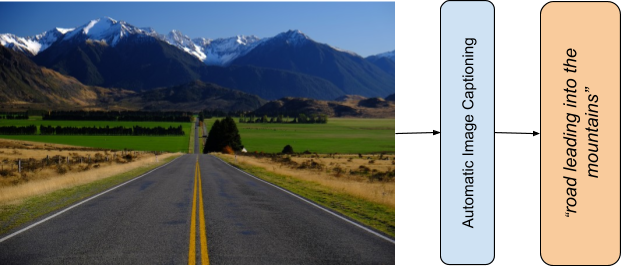
\includegraphics[width=0.6\textwidth]{figs/ch1/image-captioning.png}
	\caption{Image captioning can help millions with visual impairments by converting images captions to text. Image by \href{https://www.flickr.com/photos/francisvallance/}{Francis Vallance (Heritage Warrior)}, used under \href{https://creativecommons.org/licenses/by/2.0/}{CC BY 2.0 license}.}
	\label{fig:image-captioning}
\end{figure}

In addition to the aforementioned application of image captioning to help the visually impaired, there are many other use cases in which automatic image descriptions may help. In general, any domain in which images need to be interpreted by humans, but human availability is scarce or it is a tedious task, may benefit from an automated approach to image description.

A specific use case is the analysis and extraction of information from videos. Some video monitoring tasks are very boring and tedious. An automated mechanism to describe scenes in video footage will be of great utility for creating summaries or monitoring specific situations and events. \footnote{As an interesting example, Shell is conducting a pilot study using deep-learning to automatically monitor video footage in order to identify safety hazards and generate alerts (\href{https://customers.microsoft.com/en-us/story/shell-mining-oil-gas-azure-databricks}{link})}.

Another potential utility of automatic image description lies in the task of searching images. Having automatically generated captions for images that originally hasn't been described, would help finding images based on a complex description rather that a simple collection of tags.

\section{Goals}

This project aims at advancing in the task of automatically generating image descriptions. That is the ultimate goal of the project. However, in order to achieve such an abstract goal, we decompose it into various subgoals, as follows:

\begin{enumerate}
\item Get a solid understanding of the problem at hand and review the state-of-art solutions to it
\item Get practical knowledge on the technologies required to solve this problem
\item Develop a model using a benchmark dataset like the Flickr30K
\item Scale the model to a larger benchmark dataset such as the COCO\cite{Lin2014} dataset or the more recent Conceptual Captions Dataset by Google \cite{Sharma2018}  (see Figure \ref{fig:conceptual-captions}).
\item Evaluate the model, ideally partaking in some challenge or competition, like the ones using the COCO dataset or the Conceptual Captions dataset.
\end{enumerate}

\begin{figure}[h]
	\centering
	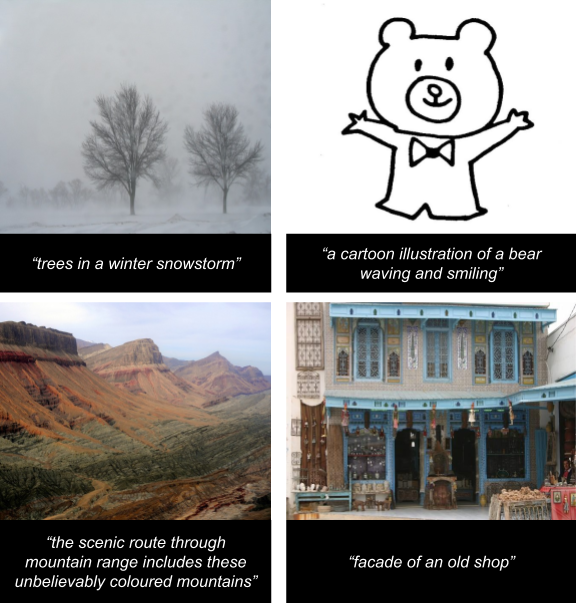
\includegraphics[width=0.6\textwidth]{figs/ch1/conceptual-captions-example.png}
	\caption{Illustration of images and captions in the Conceptual Captions dataset.Clockwise from top left, images by Jonny Hunter, SigNote Cloud, Tony Hisgett, ResoluteSupportMedia. All images used under \href{https://creativecommons.org/licenses/by/2.0/}{CC BY 2.0 license}.}
	\label{fig:conceptual-captions}
\end{figure}

\section{Methodology}

This project is mainly an academical, research-oriented project, so it would follow a process model which is common for these kind of projects, for instance, it will include a comparatively long review of the state of the art, as well as a public defense at the end. However, this project will also include the development of a software artifact to solve a data-analytic problem, therefore we should benefit from using a data-analytic model as the well known and widely adopted \textbf{CRISP-DM}. CRISP-DM, which stands for \textit{Cross-Industry Standard Process for Data Mining}, is an open standard process model and an industry-proven methodology to guide data mining projects.

As a methodology, it includes descriptions of the typical phases of a project, the tasks involved with each phase, and an explanation of the relationships between these tasks.

As a process model, CRISP-DM provides an overview of the data mining life cycle.

Figure \ref{fig:crisp-dm} depicts the relationships between the different phases of the CRISP-DM model. The sequence of the phases is not strict and moving back and forth between different phases is often required. The arrows in the process diagram indicate the most important and frequent dependencies between phases. The outer circle in the diagram symbolizes the cyclic nature of data mining itself. A data mining process continues after a solution has been deployed. The lessons learned during the process can trigger new, often more focused business questions, and subsequent data mining processes will benefit from the experiences of previous ones.

\begin{figure}[hpt]
	\centering
	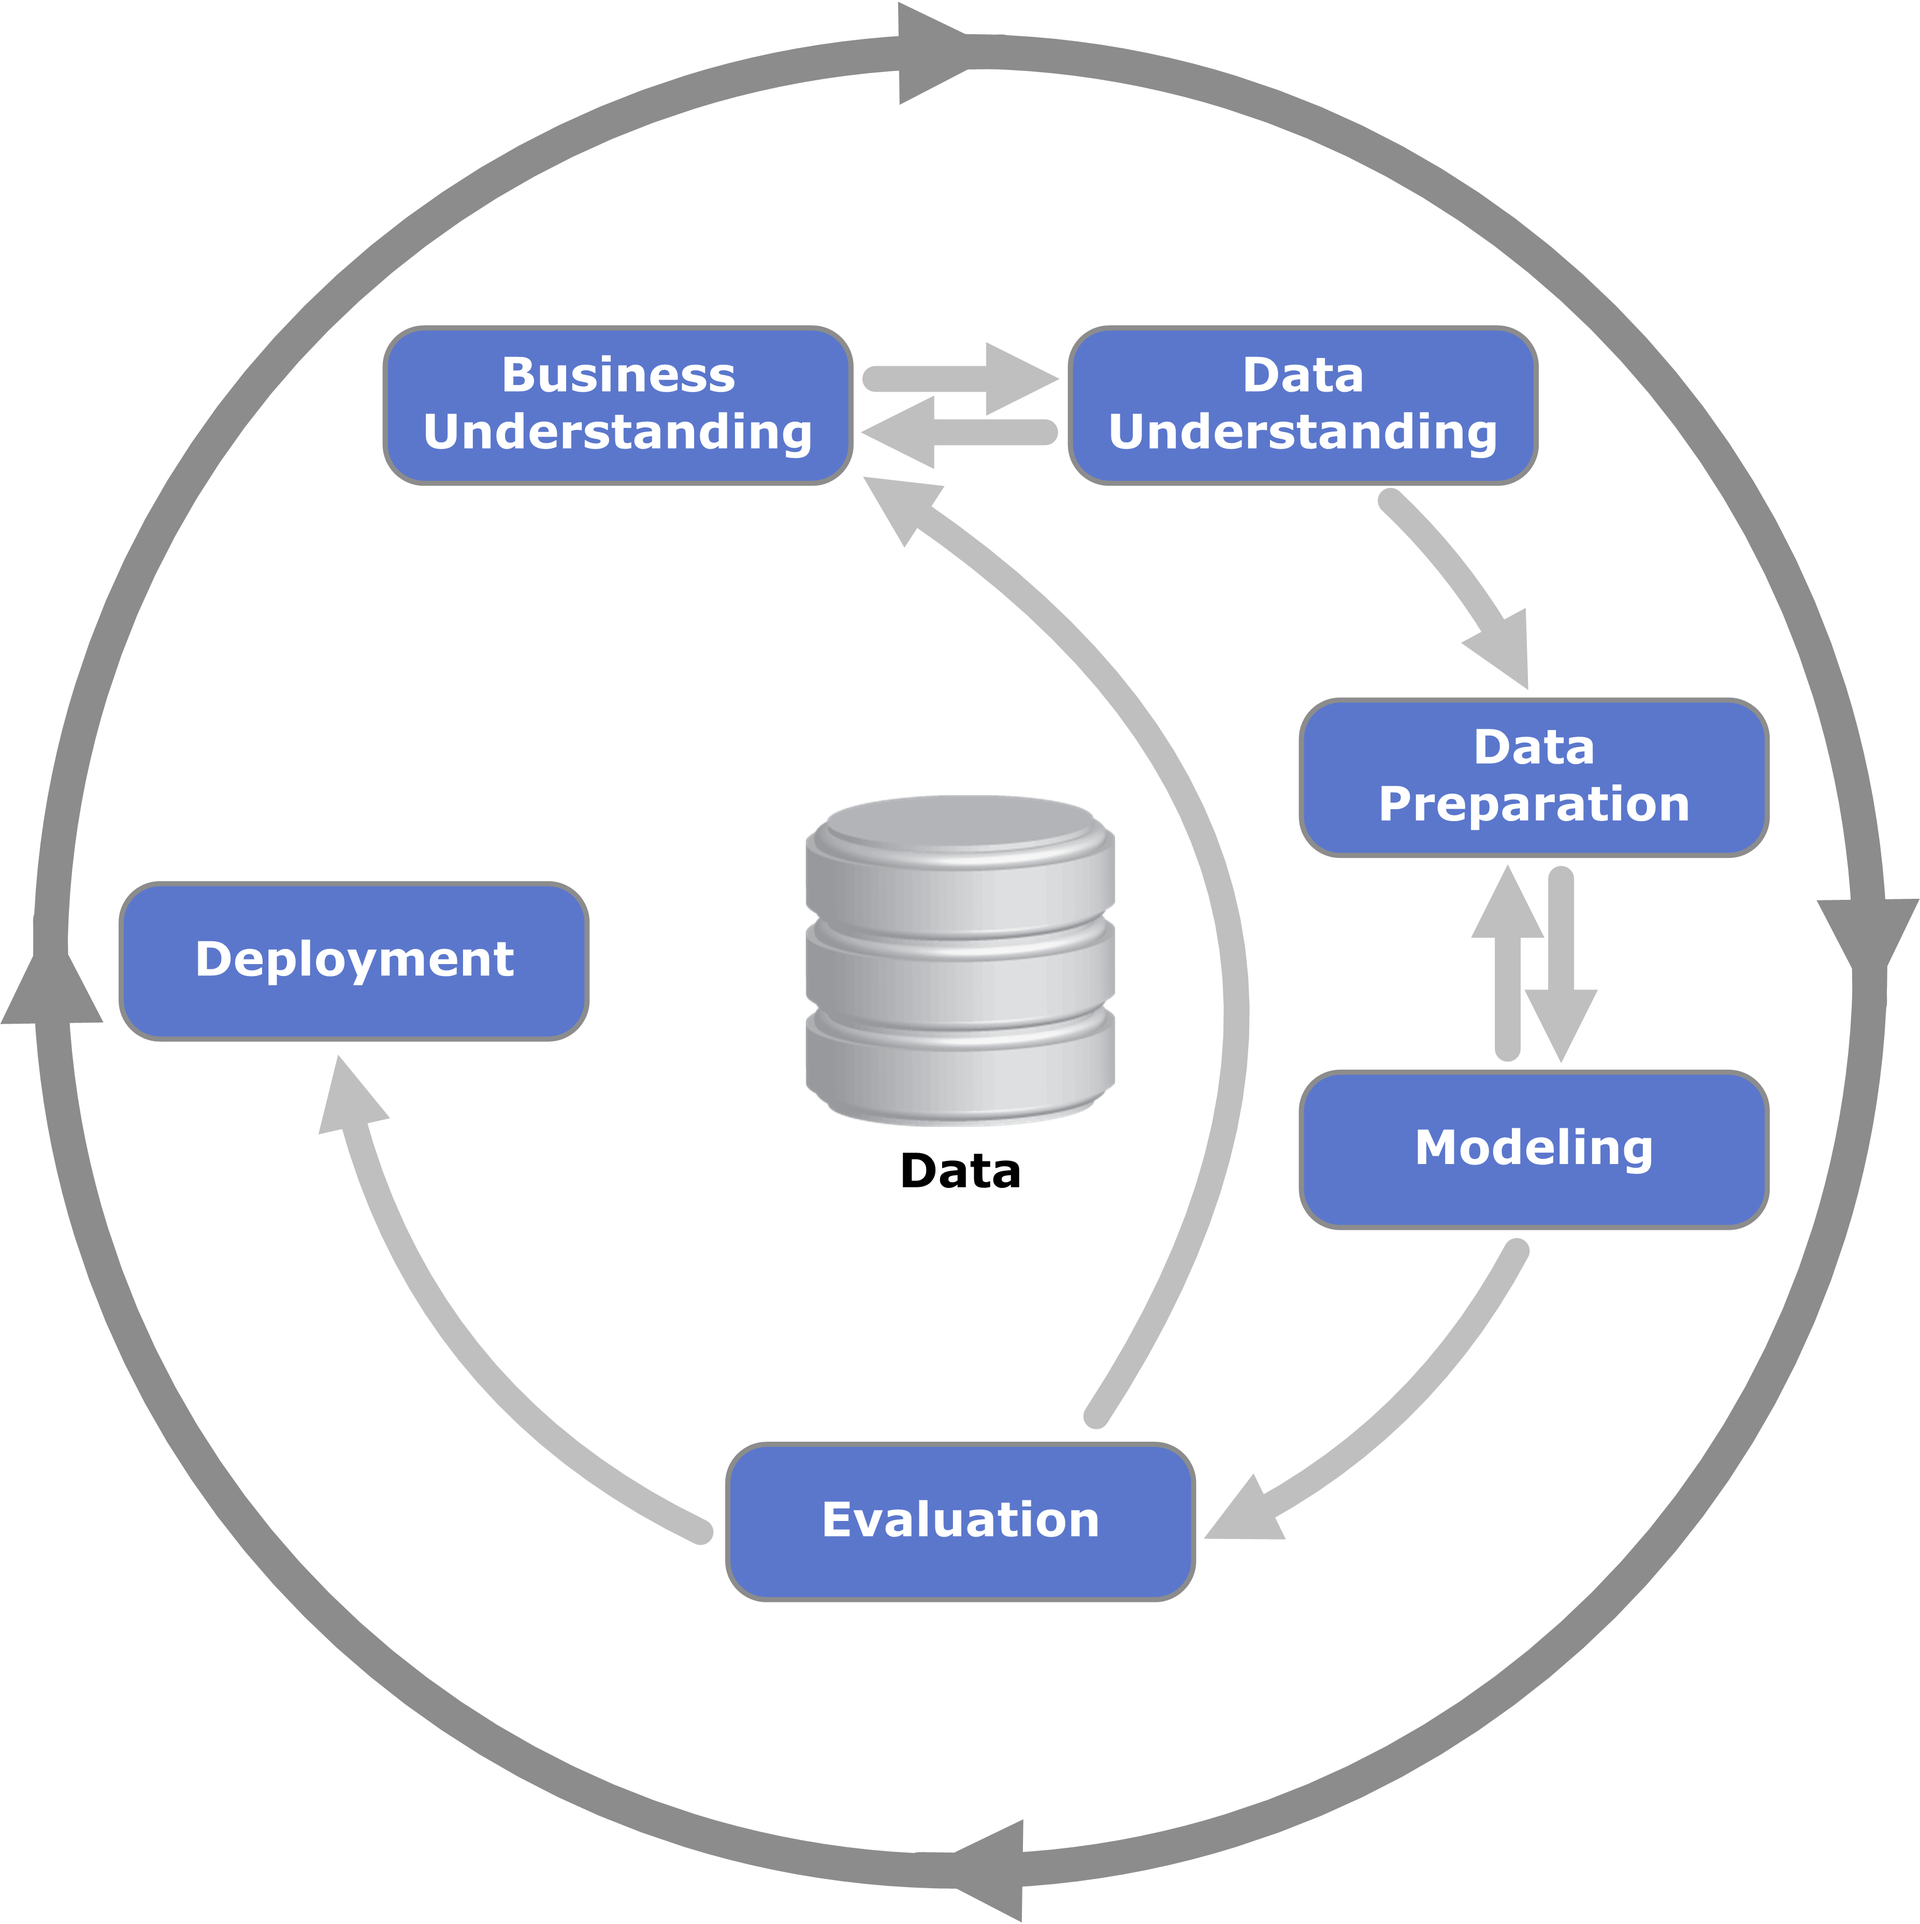
\includegraphics[width=0.6\textwidth]{figs/ch1/crisp-dm.png}
	\caption{Process diagram showing the relationship between the different phases of CRISP-DM. Image by Kenneth Jensen, used under \href{https://creativecommons.org/licenses/by/2.0/}{CC BY-SA 3.0 license..}}
	\label{fig:crisp-dm}
\end{figure}

The process model consists of six major phases:

\begin{itemize}
\item \textbf{Business Understanding}: Includes an in-depth analysis of the business objectives and needs. The situation is assessed and the goals of the project are defined. This should follow the setting up of a plan to proceed.
\item \textbf{Data Understanding}: Conduct initial or exploratory data analysis to become familiar with data and identify potential problems. Examine properties of data and verify its quality by answering questions concerning the completeness and accuracy of the data.
\item \textbf{Data Preparation}: After the data sources are completely identified, proper selection, cleansing, constructing and formatting should be done before modelling. 
\item \textbf{Modeling}: Modeling is usually conducted in multiple iterations, which involve running  several models using the default parameters and then fine-tune the parameters or revert to the data preparation phase for additional preparation. Usually, there are different ways to look at a given problem, so it is convenient to build multiple models,
\item \textbf{Evaluation}: The results of models are evaluated in the backdrop of business intentions. New objectives may sprout up owing to the new patterns discovered. This is, in fact, an iterative process, and the decision whether to consider them or not has to be made in this step before moving on to the final phase
\item \textbf{Publication}. The final information gathered has to be presented in a usable manner to the stakeholders.  This has to be done as per their expectations and business requirements.
\end{itemize}


\section{Planning}

Main tasks and milestones

\begin{table}[hbt]
\begin{tabular}{|l|l|l|}
\hline
Phase   & End  & Description   \\ \hline
1 & 3/3/2019 & Definition and planning  \\ \hline
2 & 24/3/2019 & State of the Art \\ \hline
3 & 19/5/2019 & Development \\ \hline
4 & 9/6/2019 & Complete this report \\ \hline
5 & 16/6/2019 & Presentation
\end{tabular}
\end{table}

Phase 2: this phase will encompass the following tasks:
\begin{itemize}
\item Reviewing relevant bibliography
\item Studying the problem domain (business understanding), and becoming familiar with the data. At this stage we would also start preparing the data for the modeling stage
\end{itemize}

Phase 3: this will be the longest phase, and it will include the following tasks  
\begin{itemize}
\item Preparing the data. Although data preparation could be started during phase 2, depending on the chosen models it could be necessary to conduct some additional data preparation operations
\item Generating one or various models. We plan at creating at least two models, one that would replicate existing work, and another one to explore new ideas and try to beat the baseline model.
\item Evaluating the models, and very specifically, compare our model against the replicated model.
\item Publication: We consider two courses of action: a) participating in the Conceptual Captions Challenge by Google, and b) delivering some product to the final user, although it would be a very basic prototype given the little time available.
\end{itemize}

In phase 4 we will complete this report. We would probably overlap this task with some of the tasks in phase 3 that will required more time, like the evaluation of the models and the participation in challenges.

In phase 5 we will present the results achieved for its evaluation. These results will include the code, the documentation and a public defense of the project in front of an academic board


\chapter{State of the Art}
\label{ch:state_of_the_art}

Recently there have been an upsurge of interest in problems that require a combination of linguistic and visual information. Besides, the rise of social media in the web has made available a vast amount of multimodal information, like tagged photographs, illustrations in newspaper articles, videos with subtitles, and multimodal feeds on social media. To tackle combined language and vision tasks and to exploit the large amounts of multimodal information, the CV and NLP communities have been increasingly cooperating, for example by organizing combined workshops and conferences. One such area of research in the intersection of both worlds is automatic image description.

\textbf{Automatic image description} can be defined as the task of automatically generating a description of an image using natural language. It is a very challenging problem that combines two different problems into a single task: on the one hand, there is the problem of understanding an image, which belongs to the \textbf{Computer Vision (CV)} field, one the other hand, there is also the problem of generating a meaningful and grammatically-correct description of the image, which belongs to the \textbf{Natural-Language Processing (NLP)} field, and to be more precise, it belongs to the class of \textbf{Natural-Language Generation (NLG)} problems.

Both CV and NLP are challenging fields themselves. While both fields share common techniques rooted in artificial intelligence and machine learning, they have historically developed separately, with little interaction between their scientific communities.  Recent years have seen considerable advances in both fields, to a great extent thanks to the application of deep-learning techniques and the recent advances in this area. This chapter presents a brief survey of the recent literature on this topic, including some antecedents, but focusing primarily on the recent advances coming from the application of \textbf{Deep Learning} technology, since this is our main interest.

The chapter is organized in various sections. First section is devoted to further delimiting the task at hand as well as introducing classification system for the different approaches to the problem. Subsequent sections review relevant publications organized according to the provided classification scheme. Finally, there is a section describing the datasets used by the community to benchmark their models and a short discussion on the evaluation metrics for this kind of tasks.

\section{Task definition and classification of methods}\label{sec:task-definition}

We have already defined the task of automatic image description as the task of automatically generating a description of an image using natural language generation. However, this definition is too generic to precisely characterize the task we are interested in. For example, when presented with certain image, an algorithm may generate a list of labels describing different elements of the image, or it may describe technical features of the image, such as the dimensions, the predominant colors, brightness, etc. Therefore, we need a more concrete definition of the task.

When talking about \textbf{automatic image description}, we refer to descriptions that meet three properties:
\begin{itemize}
\item Descriptions that are relevant, that is, that talk about the elements of the image.
\item Descriptions that are expressed as natural language, using grammatically correct sentences
\item Descriptions that are comprehensive but concise at the same time, that is, the description should aim at summing up the important elements of the image, not just describing it.
\end{itemize}

From the CV point of view, this task requires \textbf{full image understanding}: the description should demonstrate or pretend a good understanding of the scene, far beyond simply recognizing the objects in the image. This means that the description is able to capture relations between the objects in the scene, and the actions happening there.

From the NLP point of view, this task requires \textbf{sophisticated natural language generation} (NLG), which involves: selecting which aspects to talk about (content selection), sorting and organizing the content to be verbalized (text planning), and finally generating a semantically and syntactically correct sentence (Surface realization).

Intuitively, descriptions should be easy to understand by a person, and that person should be able to grasp the essence of the image, to create a mental model of the image without actually seeing it. The description task can become even more challenging when we take into account user-specific tailored descriptions. For instance, when describing the paintings available in a museum, a tourist may require a different description than a librarian or an art critic.

Since 2011 there have been a considerable advance in challenging CV tasks, to a great extent fostered by the application of deep learning models and the availability of large corpus of data available to researchers. More recently, a similar process seems to be occurring in the NLP field. Not surprisingly, these advances in both CV and NLP have also propelled a new wave of interest in cross-disciplinary research problems involving both areas of research, and automatic image description is a very good example. As a consequence, the CV and NLP communities have increased cooperation, for example by organizing joint workshops over the past few years. These efforts have resulted in a surge of new models, datasets and evaluation measures, which is reflected in the increase of publications, specially from 2014. 

In order of ease of review, understanding and comparison of the growing amount of research on the topic, existing surveys have proposed various schemes to classify the models being used.

One the one hand, the survey by \citet{Bernardi2017} proposes a classification system based on two dimensions and only tree categories. On the other hand, \citet{Bai2018} organize the existing research according to the kind of architecture or framework used, resulting in a more fine grained classification with 8 categories. 

After comparing both both approaches to classify the existing research, we  prefer the approach adopted by \citet{Bai2018} as we consider it more precise and descriptive,  resulting in a finer granularity; while the classification by \cite{Bernardi2017} is more abstract, resulting in a coarser granularity. A more recent survey by \citet{Hossain2019} takes the same approach found in \citep{Bai2018} with a more focused review of deep-learning based models and references to the most recent work published so far.

Below we provide a short overview of the publications covered in this survey organized into categories and sorted by publication year:

\begin{table}[ht]
\centering
\caption{Summary of published research on the automatic image description problem.}
\label{tab:overview}
\begin{tabular}[t]{p{0.3\textwidth} p{0.7\textwidth}}
    \toprule
    Approach & Representative research\\
    \midrule
    Retrieval-based & \citet{Farhadi2010, Ordonez2011, Gupta2012, Kuznetsova2012, Hodosh2013a, Kuznetsova2014, Mason2015, Hodosh2013b}\\
    Template-based &  \citet{Yang2011, Kulkarni2011, Li2011, Mitchell2012, Ushiku2015}\\
    Earlier Deep Models &  \citet{Socher2014, Karpathy2014, Ma2015, Yan2015, Lebret2015a, Yagcioglu2015}\\
    Multimodal learning & \citet{Kiros2014_VS, Mao2015_mRNN, Karpathy2015, Chen2015}\\
    Encode-Decoder framework & \citet{Kiros2014_LBL, Vinyals2015, Donahue2015, Jia2015, Wu2016, Pu2016_DGDN, Gan2017_Style, Hao2018}\\ 
    Compositional architectures & \citet{Fang2015, Tran2016, Ma2016, Oruganti2016, Wang2016_Parallel, Fu2017, Gan2017_SCN}\\
    Attention-guided & \citet{Xu2015, You2016, Yang2016_RevNet, Zhou2017, Khademi2018, Anderson2018_BUTD, Jiang2018}\\
    Describing novel objects & \citet{Mao2015_Child, Hendricks2016}\\ 
    Other deep learning methods & \citet{Pu2016_VAE, Dai2017_CGAN, Shetty2017, Ren2017, Rennie2017, Zhang2017, Anderson2018_SemiSup, Feng2018, Gu2018, Li2018_CAL, Li2018_VS-LSTM, Lindh2018}\\
    \bottomrule
\end{tabular}
\end{table}

% Skipped Wang2016_Unified, Chen2017_StrucCap, Chen2017_RLSTM, Dai2017_CL, Zhang2019, Cao2019, He2019,

\section{Early work: methods that are not based on deep learning}\label{sec:first-methods}

This section reviews the initial attempts to solve the image captioning problem. All these methods have in common that they do not use deep learning techniques. We divide them into two groups: retrieval based approaches and template-based approaches.

\subsection{Retrieval-based} \label{subsec:retrieval-based_methods}

Early work on the topic was often based in the use of retrieval-based approaches, also referred to as transfer-based approaches. These approaches usually follow a two steps process. During the first step, given a query image, a candidate set of similar images is retrieved using content-based image retrieval techniques, which are based on global image features extracted from the image. During the second step, a re-ranking of the retrieved images is computed using a variety of methods. Finally, the caption of the top image is returned, or a new caption is composed from the captions of the top-n ranked images.

\citet{Farhadi2010} use a meaning space consisting of \textit{<object, action, scene>} triplets to link images and sentences. Their model takes an input image, map it into the meaning space by solving a Markov Random Field, and use Lin's information-based similarity measure \citep{Lin1998} to determine the semantic distance between the query image and the pool of available captions. Finally, the semantically closest sentence is used as the image description.

The IM2TEXT model by \citet{Ordonez2011} uses the scene-centered descriptors of the GIST model \citep{Oliva2006, Torralba2008} to retrieve a set of similar images as a baseline, then these images are ranked using a classifier trained over a range of object detectors and scene classifiers specific to the entities mentioned in the candidate descriptions. Finally the caption of the top ranked image is returned. 

\citet{Kuznetsova2012} take on the work by \citet{Ordonez2011} with some notable twists: instead of retrieving a candidate set of images using content --visual-- features, their model start by running the detectors and scene classifiers used in the re-ranking step of the IM2TEXT model to extract and represent the semantic content of the query image. Then, instead of performing a single retrieval step to get neighbors of the query image, their model carries out a separate retrieval step for each visual entity detected in the query image. The result of this step is a collection of phrases of different type (noun and verb phrases and prepositional phrases). Finally, a new sentence is composed from a selected set of phrases using a constrain optimization approach. A refinement of the former approach is presented in \citet{Kuznetsova2014}, based on the use of tree structures to improve the sentence generation process.

\citet{Gupta2012} combine the image features of the GIST model with RGB and HSV color histograms, Gabor and Haar descriptors, and SIFT \citep{Lowe2004} descriptors for the retrieval step. Then, instead of using the visual features for the ranking step, their model relies on the textual descriptions of the retrieved images, which are segmented to obtain phrases of different type. This model takes the phrases associated to the retrieved images, rank them based on image similarity, and integrate them to get triples of the form \textit{( ((attribute1, object1), verb), (verb, prep, (attribute2, object2)), (object1, prep, object2) )}. Finally, the tree top-n triplets are used to generate an image description.

\citet{Hodosh2013b} employ a Kernel Canonical Correlation Analysis (KCCA) \citep{Bach2003} technique to project images and text items into a common space, where training images and their corresponding captions are maximally correlated. In the new common space, cosine similarities between images and sentences are calculated to rank the sentences, which are then used to select the top-n captions. This work is highly focused on the problems associated with existing benchmarks datasets and the evaluation metrics, and as a result the authors introduce a new dataset composed of 8000 images annotated with 5 captions per image, and propose a new metric based on binary judgments of image descriptions.

\citet{Mason2015} use visual similarity to retrieve a set of candidate captioned images. Second, a word probability density conditioned on the query image is computed from the retrieved captions. Finally, the candidate captions are scored using the word probability density and the one with the highest score is selected. 

An detailed analysis of the literature reviewed here reveals at least two dimensions that may further help in understanding and organizing the research: on the one hand, some approaches simply select one of the retrieved sentences as the image caption, while others compose a new caption by combining elements from several sentences; on the other hand, some approaches use visual detectors to find similar images (Content-Based Image Retrieval), while other approaches use conceptual information (Concept-Based Image Retrieval), or use a combination of visual and conceptual information for the retrieval step. \Cref{tab:retrieval-classification} sums up the various dimensions used to classify retrieval-based methods to the image captioning problem.

\begin{table}[ht]
\centering
\caption{Classification of retrieval-based image captioning.}
\begin{tabular}[t]{p{0.3\textwidth}p{0.35\textwidth}p{0.35\textwidth}}
    \toprule
    Approach & Representative research\\
    \midrule
    Information modality & Select one caption & Compose caption \\
    Visual & \citet{Farhadi2010, Mason2015} & \cite{Gupta2012} \\
    Conceptual &  \cite{Ordonez2011} & \citet{Kuznetsova2012, Kuznetsova2014} \\
    Hybrid &  \citet{Hodosh2013b} & \\
    \bottomrule
\end{tabular}
\label{tab:retrieval_classification}
\end{table}

The main disadvantage of Retrieval-Based approaches comes from its reuse of existing images. The sentences used to describe images in the past may be completely inadequate for describing a new image. Although some of the proposed models are able to compose new sentences rather than just returning one of the stored sentences, these are still based on previously used sentences, so the result may still be unsuited for describing the query image. This limitation was specially evident with the use of small datasets, therefore, perhaps the problem would be alleviated with the use of very large datasets as the ones that have appeared recently \citet{Lin2014, Sharma2018}.

\subsection{Template-based approaches}\label{subsec:template-based_methods}

Another group of early attempts to solve the automatic image captioning problem take some kind of template-based approach. Unlike retrieval based approaches, template-based approaches analyze the query image to generate concepts, and then use some kind of constraining mechanism to compose a sentence. The constrains typically adopt the form of a template, but can also be specified as grammar rules.

For example, \citet{Yang2011} use a quadruplet consisting of \textit{<Noun-Verb-Scene-Preposition>} as template for generating image descriptions. The process starts with the execution of detection algorithms to estimate objects and scenes in the image, and then apply a language model trained over the Gigaword corpus\footnote{https://catalog.ldc.upenn.edu/LDC2003T05} to compute nouns, verbs, scenes and prepositions that might appear in the caption. Finally, they apply Hidden Markov Model Inference to compute probabilities for all the elements, and use the elements with the highest probabilities to fill the template and generate a new sentence.

\citet{Kulkarni2011} employ Conditional Random Field (CRF) to determine image contents, which results in a graph with nodes corresponding to objects in the image, object attributes, and spatial relationships between objects. Unary potential functions are computed for nodes in the graph, while pairwise potential functions are obtained on a collection of existing descriptions. Afterwards, CRF inference is used to determine the image contents to be described, and finally a sentence template is applied to generate sentence using the selected content.

\citet{Li2011} use visual models to detect objects, attributes and spatial relationships, and. Then, they resort to web-scale n-gram data to compute frequency counts of possible n-gram sequences to fill a triplet defined as \textit{<(adj1, obj1), prep, (adj2, obj2)>}. Finally, dynamic programming is applied to find an optimal set of phrases that constitute the description of the query image.

\citet{Mitchell2012} apply algorithms that are able to represent an image as an <objects, actions, spatial relationships> triplet. Syntactically informed word co-occurrence statistics are computed and used by a sentence generator to filter and constrain the output of the image processor using tree structures.

The aforementioned works in this section produce new sentences based on individual words (nouns, adjectives, verbs, prepositions, etc.) that generated in a piece-wise manner from the query image, and these words are later connected according to certain grammar model. To improve on this approach, some authors have proposed the use of phrases instead of individual words. In particular, \citet{Ushiku2015} present a method named Common Subspace for Model and Similarity (CoSMoS). CoSMoS obtains a subspace in which all feature vectors associated with the same phrase are mapped as mutually close, classifiers for each phrase are learned, and training samples are shared among co-occurring phrases. Phrases estimated from a query image are connected by using multi-stack beam search to generate a description.

Template-based approaches to automatic image captioning may improve the relevance of the resulting captions when compared with retrieval based approaches, template-based captions tend to be too rigid, thus resulting in a lack of naturality when compared to human-written sentences.

\section{Deep-learning approaches}\label{sec:deep-learning_methods}

Convolutional Neural Networks (CNN) were first introduced by Yann LeCun in 1998 \citep{Lecun1998}, but it was not until more than a decade later than they started to shine. In 2012, a large, deep CNN \citep{Krizhevsky2012} was used to win, by a incredibly wide margin, the 2012 ImageNet Large-Scale Visual Recognition Challenge. From that turning point, the field has attracted attention of researchers from various fields and gained howling popularity. The success of CNN and other deep learning models was due to a great extent to its impressive results in many challenging problems, specially in the fields of Computer Vision and Natural Language Processing, where deep-learning models have became the state of the art. Not surprisingly, researchers have attempted to apply deep neural networks to solve problems in the interstice of both fields, CV and NLP, includes the problem of automatically generating image descriptions.

Recent advances in the field have been achieved with the introduction of new architectures and frameworks, accompanied by increasingly larger datasets to feed those deep neural networks. Therefore, there is a wide repertoire of methods for tackling the image captioning tasks. This section presents the contributions to the field organized according to the kind of architecture or framework utilized, with one subsection per category

\subsection{Earlier Deep Models}\label{subsec:earlier_deep-learning_models}

Encourage by the success of CNNs to solve image classification tasks, researchers began incorporating deep models into their image captioning methods, yet still influenced by the retrieval-based and template-based methods. Image captioning was formulated as a multi-modality embedding \citet{Frome2013} and ranking problem.

\citet{Socher2014} use dependency-tree recursive neural networks (DT-RNN) to represent phrases and sentences as compositional vectors. Another deep neural network \citep{Le2013} is used to extract visual features from the images. Both types of  features are mapped into a common space by using a max-margin objective function. After training, sentence retrieval is performed based on similarities between representations of images and sentences in the common space.

\citet{Karpathy2014} introduce a twist in the previous model by working at a finer level, that is, instead of modelling full images, they work on a finer level by embedding fragments of images as well as fragments of sentences fragments into a common space.  An structured max-margin objective is used to explicitly associate these fragments across modalities. Image fragments are obtained by means of a Region CNN \citep{Girshick2014}. Sentence fragments are modelled as typed dependency tree relations \citep{DeMarneffe2006}. At last, a retrieval task is performed by computing image-sentence similarities that combine both a global term and a fragment-aligned term. Experimental evaluation showed that reasoning on both the global level of images and sentences and the finer level of their respective fragments improves performance on the image-sentence retrieval task.

\citet{Ma2015} take into consideration different levels of interaction between images and sentences in order to compute similarities. Their architecture combines two different deep neural networks to tackle the multimodal space: an image encoding CNN \citep{Simonyan2015} to encode visual data, and a matching CNN \citep{Hu2014} to learn the joint representation of images and sentences. The matching CNN composes words to different semantic fragments and learns the inter-modal relations between image and the composed fragments at different levels. 

\citet{Yagcioglu2015} propose a query expansion approach for improving transfer-based automatic image captioning. The core idea of this method is to translate the given visual query into a distributional semantics based form, which is generated by the average of the sentence vectors extracted from the captions of images visually similar to the input image. It is a data-driven approach, that extracts image features using the Caffe architecture \citep{Jia2014}, a Region-CNN pipeline trained on the ImageNet dataset. The original query is expanded as the average of the distributed representations of the captions associated with the retrieved descriptions \citep{Mikolov2013}, weighted by their similarity . Finally, they transfer the closest caption as the description of the input image.

\citet{Devlin2015} also utilizes CNN activations as the global image descriptor, and perform k-NN retrieve images in the training set that are similar to the query image. Then their model selects a description from the candidate descriptions associated with the retrieved, just like the approaches by \citet{Mason2015} and \citet{Yagcioglu2015}. Their approach differs in terms of how they represent the similarity between description and how they select the best candidate over the whole set. Specifically, they propose to compute the description similarity based on the \textit{n-gram} overlap \textit{F-score} between the descriptions. The model returns the description with the highest mean n-gram overlap with the other candidate descriptions, that is the one associated to the k-NN centroid.

\subsection{Multimodal learning}\label{subsec:multimodal-learning}

Retrieval-based and template-based methods to image captioning impose limitations on the capacity to describe images in the form of templates, structured prediction, and/or syntactic trees. Thanks to the advances in neural networks, new approaches emerged that were able to surpass those limitations. These methods can yield more expressive and flexible sentences with richer structures.  Multimodal neural language models constitute one way of approaching the problem from a learning perspective. In general, these models are bidirectional, that is, they are able to generate new captions for an image, but they can also be applied in retrieval tasks for both images and sentences.

\begin{figure}[hpt]
	\centering
	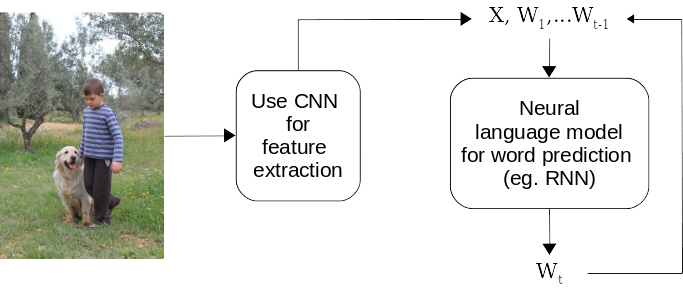
\includegraphics[scale=0.5]{ch2/multimodal.png}
	\caption{Structure of multimodal neural learning models for image captioning}
	\label{fig:multimodal}
\end{figure}

General structure of multimodal neural-based learning is shown in \cref{fig:multimodal}. First, image features are extracted using a feature extractor, typically a CNN. Then, the extracted features are forwarded to a neural-based model, which maps the image features into a common space with the word features. Finally, the model predicates new words based on the image feature and previously generated context words.

\citet{Kiros2014_VS} use a CNN for extracting image features using a multimodal space that jointly represents image and text. The key to achieve that is the use of Multimodal Neural Language Models (MNLM), that is, models of natural language that can be conditioned on other modalities. An image-text multimodal neural language model can be used to retrieve images given complex sentence queries, retrieve phrase descriptions given image queries, as well as generate text conditioned on images. The authors introduce two such languages that are adaptations of the Log-Bilinear Language Model proposed by \citet{Mnih2007}. In the case of image-text modelling it is possible to jointly learn word representations and image features by training the models together with a CNN like AlexNet \citep{Krizhevsky2012}.

\citet{Mao2014, Mao2015_mRNN} present a multimodal Recurrent Neural Network (m-RNN) model for generating novel image captions. It directly models the probability distribution of generating a word given previous words and an image, and uses this distribution to generate image captions. The model consists of two sub-networks: a deep RNN for sentences and a deep CNN for images. These two sub-networks interact with each other in a multimodal layer to form the whole m-RNN model. Besides generating captions, the m-RNN model can be applied for retrieving images or sentences. This model achieved state of art results across image captioning and image and caption retrieval tasks.

\citet{Karpathy2015} propose another multimodal approach using deep neural networks to learn embedding of image and natural language data for the task of bidirectional images and sentences retrieval. However, unlike previous methods that embed full images and sentences, this method works at a finer level, by working with fragments of images and fragments of sentences. This method applies Region-CNN to break down an image into a number of objects, RNN over sentences, represented by a dependency tree relations (DTR) \citep{DeMarneffe2006}, and a structured objective that aligns the two modalities through a multimodal embedding. The resulting Multimodal RNN architecture learns to generate novel descriptions of image regions. This model outperformed retrieval baselines on full images as well as images annotated with region-level sentences, which were derived from the MSCOCO dataset.
 
\citet{Chen2015} also explore the bi-directional mapping between images and their textual descriptions. This approach uses a RNN that attempts to dynamically build a visual representation of the scene as a caption is being generated or read. The representation automatically learns to remember long-term visual concepts. This model is capable of both generating novel captions given an image, and reconstructing visual features given an image description. The model was tested on several tasks, including sentence generation, sentence retrieval and image retrieval, and achieved state-of-the-art results for the task of generating novel image descriptions. The results for the image and sentence retrieval tasks were comparable to state-of-the-art methods using similar visual features.

In general, the multimodal approaches have limitations to handle a large amount of data and are inefficient to work with long term memory.

\subsection{The Encoder-Decoder framework}\label{subsec:encoder-decoder_framework}

The \textbf{encoder-decoder framework} was originally designed to translate sentences between different languages \citep{Kalchbrenner2013, Sutskever2014, Cho2014}. Inspired by its success solving translation problems, some researchers have adopted them to generate image captions with great success. The idea behind adapting this framework designed for translation tasks, was to see the image captioning tasks also as translation problem but across different modalities. 

\begin{figure}[hpt]
	\centering
	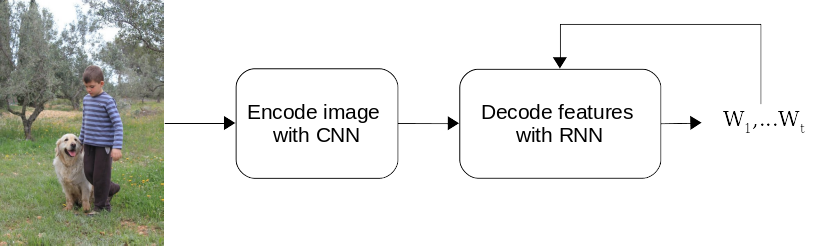
\includegraphics[scale=0.5]{ch2/encoder-decoder.png}
	\caption{Structure of image captioning methods based on the encoder-decoder framework}
	\label{fig:encoder-decoder}
\end{figure}

\citet{Kiros2014_LBL} were the first to apply the encoder–decoder framework to generate image descriptions by unifying joint image-text embedding models and multimodal neural language models. The idea is that given an image input, a sentence output can be generated word by word, like in language translation. Their model uses a Long Short-Term Memory (LSTM) \citep{Hochreiter1997} to encode textual data, and a CNN to encode visual data. Then, by optimizing a pairwise ranking loss, encoded visual data is projected into an embedding space spanned by LSTM  hidden states that encode textual data. In the embedding space, a multimodal neural language model --the so called Structure-Content Neural Language Model (SC-NLM)-- is used to decode the visual features conditioned on context word feature vectors, thus allowing for word-by-word generation of a sentence. This method achieved significant improvements in generating realistic image captions over the multimodal neural language models proposed in \citep{Kiros2014_VS}.

\citet{Vinyals2015} propose a method similar to the one by \citet{Kiros2014_VS}, which uses a CNN for image representations and an LSTM for generating image captions. This method, referred trains the LSTM based on maximum likelihood estimation. The LSTM works as follows: (1) image information is included into the initial state of the LSTM; (2)next words are generated based on the current time step and the previous hidden state; (3) this process continues until it gets the end token of the sentence. 

A problem with the former encoder-decoder methods is their susceptibility to the vanishing gradient problem, due to  image information being fed only at the beginning of the process. Consequently, the role of the initial words is also becoming weaker and weaker as the process continues. Therefore, the captions tend to degrade in relevance when generating long sentences. With the aim of mitigating this problem, \citet{Donahue2015} introduce a variation into the encoder-decoder architecture that stacks multiple LSTM atop one another. Rather than projecting the vision space into the embedding space of the hidden states at the initial stage, this model takes a copy of the static image and the previous word directly as input, that is then fed to the stack of LSTMs at each time step. This architecture, referred to as the Long-term Recurrent Convolutional Network (LRCN) model, is able to process not just static images, but also dynamic tasks involving sequences, like videos.

Still playing around with the encoder-decoder framework, some researchers propose methods to augment it by including high level semantic concepts explicitly. 

\citet{Jia2015} propose an extension of the LSTM model, which they call guided LSTM of gLSTM for short. This model adds semantic information from the image, and this information is included as extra input to each gate and cell state of the LSTM network, with the aim of guiding the model towards more relevant solutions, specially when generating long sentences. Semantic information is extracted in different ways. One way is by means of a cross-modal retrieval task that first retrieves image captions and then extracts semantic information from these captions Another way is by using a multimodal embedding space. Besides, this work explores different length normalization strategies for beam search to avoid bias towards short sentences, obtaining results that are on par with or better than the current state-of-the-art.

\citet{Wu2016} also incorporate high-level semantic concepts into the encoder–decoder framework in the form of attribute probabilities. To this end, the authors first mined a set of semantic attributes based on words commonly found in image captions. Second, they trained a multi-label classifier using one CNN per attribute, to predict the probability of attributes being present in the image. The trained CNNs are used to create a vector for each image that represents the probability of each attribute being present in it. For the caption generation, prediction vector is passed to an LSTM. For different tasks, different language models may be used, and specifically, for image captioning they adopt the region-based multi-modal language model by \citet{Vinyals2015}. The model is also capable to incorporate external semantic information and doing so further improves performance.

A circumstance that may limit the practical application of the majority of approaches discusses so far will occur when the availability of captions is limited to just a fraction of the available images. In that case, a semi-supervised learning approach would be of significant practical values. With that situation in mind, \citet{Pu2016_VAE} propose a semi-supervised learning method under the encoder–decoder framework. This method uses a Deep Generative Deconvolutional Network (DGDN) \citep{Pu2016_DGDN} as a decoder of the latent image features, and a deep CNN as an image encoder; the CNN is used to approximate a distribution for the latent DGDN features. The latent features are also linked to generative models of captions by the RNN decoder. To generate captions for new images, averaging is performed across the distribution of latent features. This framework is capable of modeling the image in the absence of associated captions, thus this is semi-supervised setting for CNN learning with images. 

\subsection{Attention-guided models}\label{sec:attention-guided_models}

Image captions should be kept short but informative. Therefore, such descriptions should mention only the most salient elements of the image, and avoid small details. Motivated by the visual attention mechanism of primates and humans \citep{Rensink2000, Spratling2004} , approaches that utilize attention to guide image description generation are proposed. By incorporating attention to the encoder–decoder framework, sentence generation will be conditioned on hidden states that are computed based on attention mechanism. The general structure of attention-guided image captioning methods is depicted in \cref{fig:attention-based} . In such methods, attention mechanism based on various kinds of cues from the input image are incorporated to make the decoding process focus on certain aspects of the input image during the caption generation process.

\begin{figure}[hpt]
	\centering
	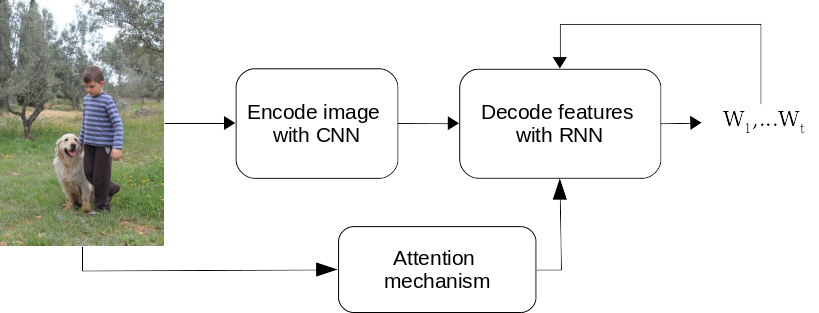
\includegraphics[scale=0.5]{ch2/attention-based.png}
	\caption{Structure of image captioning methods based on the encoder-decoder framework}
	\label{fig:attention-based}
\end{figure}

Encouraged by successes of other tasks that employ attention mechanism \citet{Mnih2014, LeiBa2015}, \citet{Xu2015} were the first to introduce an attention-mechanism to the problem of automatic image captioning. Their model, which is a variation of the encoder-decoder framework, is capable of dynamically attending salient image regions while generating the description of the image. While most approaches based on CNN image encoders use the top layer of the ConvNet for extracting image features, this method generates context vectors by using the features learned at lower layers of the ConvNet. The idea behind this approach is that the use of the top layer may result in the loss of details which may actually be useful for generating image descriptions. \citeauthor{Xu2015} have tried two different techniques for simulating attentions: stochastic hard attention and deterministic soft attention.

It is possible to classify many of the methods used in image captioning as either bottom-up or top-down. In the top-down paradigm \citep{Donahue2015, Karpathy2015, Chen2015, Mao2015_mRNN, Mao2015_Child, Vinyals2015,Xu2015} visual features are extracted first and used to select or generate a caption. In the bottom-up paradigm \citep{Farhadi2010, Kulkarni2011, Li2011, Kuznetsova2012, Elliott2013, Lebret2015a} visual concepts (e.g., regions, objects, and attributes) are extracted first and combined later to generate a caption. Top-down approaches have difficulties to deal with the fine details of an image. Bottom-up approaches, on the other hand, can operate at any image resolution and therefore are more suited for dealing with  fine details of the image. However, they have problems in formulating an end-to-end process. To take advantage of the complimentary properties of both approaches, \citet{You2016} propose a semantic attention-based method that is designed to provide a detailed, coherent description of semantically important objects. On the one hand, the visual concepts are collected using K-NN image retrieval for computing global --non-parametric-- visual concepts, and a fully convolutional network (FCN) \citep{Long2015} is trained to predict region attributes. With each attribute corresponding to one entry of the used vocabulary, words and image attributes share the same vocabulary. Under the encoder–decoder framework, the visual concepts are only forwarded to the encoder at the initial step. In the decoding stage, an LSTM is applied to decode the image features using both the global visual concepts, and the local attributes. The LSTM decoder uses two functions to generate words: an output attention function that modulates attribute attention based on the hidden state of the LSTM, and an input feedback mechanism that modulates attribute attention based on the previous word. Compared with the method introduced by \citet{Xu2015}, which works on fixed and predefined spatial location, this semantic attention-based method can work on any resolution and any location of the image.

Arguing that attention-enriched encoder–decoder models lack global modelling abilities due to their sequential information processing, \citet{Yang2016_RevNet} propose a new model called review network, which results of augmenting the encoder–decoder framework with a review module. The review network is generic and can enhance any existing encoder-decoder model.
This model performs a number of review steps with attention mechanism on the encoder hidden states, and outputs a thought vector after each review step. These thought vectors are introduced to capture the global properties of the image in a compact vector representation that is used as the input of the attention mechanism in the decoder. For example, the first review step can review what are the objects in the image?, then it can review the relative positions of the objects, and another review can extract the information of the overall context of the image. Another role for the thought vectors is as a focus for multitask learning.

\citet{Pedersoli2017} propose an area based attention mechanism for image captioning. Previous attention based methods map image regions only to the hidden state of the RNN language model. This approach, however, allows a direct association between caption words and image regions by modeling the dependencies between between image regions, caption words, and the hidden states. This associates makes the model capable of predicting the next word as well as corresponding image regions in each time-step. Another contribution of this work is the introduction of spatial transformation networks that allow for image-specific attention areas (while previous attention mechanisms used CNN activation grids, object proposals), and can be trained jointly with the rest of the network. This combination of techniques together yield state-of-the-art results on the MSCOCO dataset.

\citet{Lu2017} proposed another attention-based mechanism for image captioning using a visual sentinel. Other attention-based methods focus on the image in every time step of the recurrent neural network. However, in practice there are some words that do not need visual information (e.g. some prepositions and articles), thus applying attention to the image in these steps may be misleading and diminish the overall effectiveness of the caption generation process. To deal with this drawback, \citeauthor{Lu2017} introduce an adaptive mechanism to dynamically determine when to look at the image, and when to relay just on the language model to generate the next word. The proposed model combines a new spatial model that is able to determine where to look and a sentinel gate, which determines when to look at the image. The adaptive attention mechanism is introduced as an extension of the decoder LSTM that generates "visual sentinel" vectors (instead of just a hidden state) fallback option for the decoder. The "sentinel gate" is responsible of deciding whether to look at the image and how much information to get from it, or on the contrary, whether to relay on the visual sentinel for the caption generation process.

As we have seen, various attention mechanisms have successfully been added to deep models for improving the generation of image captions. These deep models learn dynamic weightings of the input vectors, which allow for more flexibility and expressive power than other models. Attention maps between the language space and the and language space are supposed to contain relevant information that could be useful in understanding and improving deep learning models in problems involving image and natural language, such as the image captioning problem. 

With the aim of advancing in the understanding and utility of attention mechanisms in image captioning, \citet{Liu2017_SAM} propose a quantitative method to evaluate the correctness of attention maps, which is defined as the consistency between attention maps and the corresponding regions that the words/phrases describe in the image. More specifically, \citeauthor{Liu2017_SAM} use the alignment annotations between image regions and noun phrase caption entities provided in the Flickr30k Entities dataset \citep{Plummer2015} as  ground truth maps. Using that metric, the attention-based model by \citet{Xu2015} performs better than the uniform attention baseline, but still has room for improvement in terms of attention consistency with human annotations. To improve the quality of attention maps, the authors propose the use of supervised attention, with two types of supervision: strong supervision with alignment annotation, and weak supervision with semantic labelling. In experiments, the method shows that supervised attention model performs better in mapping attention as well as image captioning tasks.

\citet{Chen2017_SCA} argue that existing visual attention based solely on spatial features have some drawbacks. To begin with, these methods compute weighted pooling only on attentive feature maps, which results in a gradual lose of spatial information. Moreover, these methods use the spatial information from the last convolution layer of the CNN, whose receptive fields correspond to very large regions, with very narrow gaps between regions; therefore, they do not get significant spatial attentions for an image. To deal with these limitations, \citeauthor{Chen2017_SCA} propose a method that combines both an spatial attention mechanism with a channel-wise attention mechanism. The new method, named SCA-CNN, extracts features not just from spatial locations, but also from different channels and multiple layers of the CNN. In addition, each filter of a convolutional layer acts as semantic detector \citep{Zeiler2014} while other methods use external sources for obtaining semantic information. In the task of image captioning, SCA-CNN dynamically modulates the sentence generation context in multi-layer feature maps, encoding where (i.e., attentive spatial locations at multiple layers) and what (i.e., attentive channels) the visual attention is. This methods outperformed visual attention-based image captioning methods across the Flickr30K and MSCOCO datasets.

To bridge the gap between humans and machines in image understanding and describing, \citet{Tavakoliy2017} study the agreement between bottom-up saliency-based visual attention and object referrals in scene description constructs. As a result of the study, \citeauthor{Tavakoliy2017} propose a saliency-boosted image captioning model that investigates possible benefits from low-level cues in language models. There are two main conclusions of the study: first, that humans mention more salient objects earlier than less salient ones in their descriptions; and second, the better a captioning model performs, the better attention agreement it has with human-generated descriptions. The authors found that the proposed saliency-boosted model does not improve significantly when the task is well learnt, but they observed a better generalization of their model when applied upon unseen data.

Visual attention plays an important role to understand images and demonstrates its effectiveness in generating natural language descriptions of images. On the other hand, recent studies show that language associated with an image can steer visual attention in the scene during our cognitive process. Inspired by this, \citet{Mun2017} introduce a text-guided attention model which learns to drive visual attention using associated captions. This model introduces an exemplar- based learning approach that retrieves from training data associated captions with each image, and use them to learn attention on visual features. This attention model enables to describe a detailed state of scenes by distinguishing small or confusable objects effectively. 

The are two main approaches to attention-based mechanisms: either use the low-level visual features to localize objects \citep{Xu2015, Lu2017}, or utilize the high-level semantic features to describe objects’ attributes \citep{Wang2017, Wu2016}, whilst the inner connections of these two types of features are not utilized. Inspired by the visual
processing of our cognitive system, \citet{Li2018_VS-LSTM} propose a model that combines low-level visual features and high-level semantic features  (attributes). The former are extracted by a Region Proposal Network (RPN), the latter are obtained by a CNN. The caption generation module is an LSTM with visual and semantic cells. The visual cell LSTM utilizes the visual features to localize the objects in the image, whilst the semantic cell LSTM further integrates the localized objects with their attributes to generate corresponding words. In addition, this method also uses Reinforcement Learning (the REINFORCE algorithm \citep{Sutton1999}) to explore proper vocabularies in the training process. The RL operates by introducing state perturbations to the LSTM units.

Top-down attention-mechanisms for building visual attention maps typically focus on some selective regions obtained from the output of one or two layers of a CNN. The input regions are of the same size and have the same shape of receptive field. \citet{Anderson2018_BUTD} argue that this approach has little consideration for the content  of the image and propose a new method inspired by the human visual system. Recent studies on human attention \citep{Buschman2007} indicate that human attention can be focused volitionally by top-down signals determined by the task at hand (e.g., looking for something), and automatically by bottom-up signals associated with unexpected, novel or salient stimuli. Inspired by this findings, \citeauthor{Anderson2018_BUTD} introduce a top-down mechanism based on Faster R-CNN \citet{Ren2015}. This mechanism proposes image regions, each with an associated feature vector, while a top-down mechanism determines feature weightings. Therefore, this method can attend both object level regions as well as other salient image regions. 

\citet{Hao2018} propose a another model based on the popular encoder-decoder architecture, but it uses the recently proposed densely convolutional neural network (DenseNet) to encode the feature maps. Meanwhile, the decoder uses an LSTM to parse the feature maps and converse them into textual descriptions. This model predicts the next word in the description by taking the effective combination of feature maps with word embedding of current input word by a visual attention switch.

\citet{Khademi2018} present a context-aware attention-based methods that employs a Bidirectional Grid LSTM (BiGrLSTM), which takes visual features of an image as input and learns complex spatial patterns based on two-dimensional context, by selecting or ignoring its input. In addition, this method leverages a set of local region-grounded texts obtained by transfer learning. The region-grounded texts often describe the properties of the objects and their relationships in an image. To generate a global caption for the image, this method integrates the spatial features from the Grid LSTM with the local region-grounded texts, using a two-layer Bidirectional Grid LSTM. The first layer models the global scene context such as object presence. The second layer utilizes a dynamic spatial attention mechanism to generate the global caption word-by-word, while considering the caption context around a word in both directions. Unlike recent models that use a soft attention mechanism, this attention mechanism considers the spatial context of the image regions.

\citet{Jiang2018} propose an extension of the encoder-decoder framework by adding a component called guiding network. The guiding network models the attribute properties of input images, and its output is leveraged to compose the input of the decoder at each time step. The guiding network can be plugged into the current encoder-decoder framework and trained in an end-to-end manner. Hence, the guiding vector can be adaptively learned according to the signal from the decoder, making itself to embed information from both image and language. Additionally, discriminative supervision can be employed to further improve the quality of guidance.

\subsection{Compositional architectures}\label{subsec:compositional_architectures}

Most of the neural methods for image captioning described in the previous sections are end-to-end systems made of tightly coupled modules whose parameters are trained jointly. An alternative architectonic approach to build such systems is based on the notion of compositional architectures, which consist of independent, loosely coupled components connected through a pipeline, where each component provides data to the next component until a final result is obtained. The idea behind this architecture is to make modular systems where it is easier to reuse existing components and replace components with little effort.

General structure of compositional image captioning methods is depicted in \cref{fig:compositional}. Usually, there are three components: 
\begin{enumerate}
\item A visual model that obtains visual features from the query image.
\item A natural language model that generates captions for the extracted features
\item A ranking module that re-ranks generated captions using a multimodal similarity model.
\end{enumerate}

\begin{figure}[hpt]
	\centering
	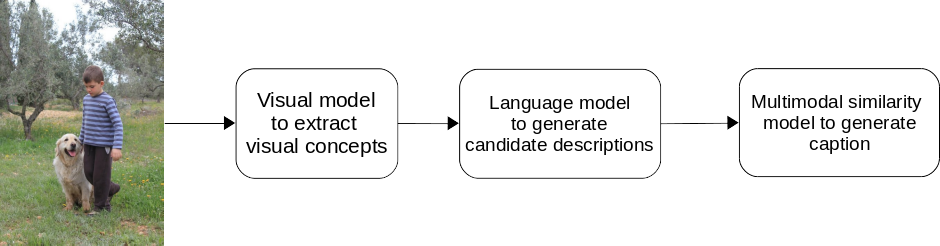
\includegraphics[scale=0.5]{ch2/compositional.png}
	\caption{Structure of image captioning methods based on the encoder-decoder framework}
	\label{fig:compositional}
\end{figure}

\citet{Fang2015} describe a system that consists of three models: visual detectors, language models and multimodal similarity models. The training process consists of two steps: First, a vocabulary of words that are most common in the training captions. Second, a visual detector is trained for each word in the vocabulary using multiple instance learning  \citep{Viola2005}. Once trained, the system can be used to generate image captions: A CNN \citep{Krizhevsky2012} is used to obtain visual features expressed as words learned vocabulary, then a maximum entropy language model \citep{Berger1996} is applied to generate candidate captions conditioned on those features. During this process, left-to-right beam search \citep{Ratnaparkhi2000} with a stack of pre-specified length $l$, produces $l$ candidate descriptions. Finally, a deep multimodal similarity model, which maps images and text fragments into a common space for similarity measurement, is used to re-rank the candidate descriptions and select the top one.

Taking on the same architecture introduced by \citet{Fang2015}, \citet{Tran2016} present a system specialized in describing landmarks and celebrities. However, instead of a CNN for the visual feature detector, this model uses a deep residual network (ResNet) to detect a broader range of visual concepts \cite{He2016a}, a maximum entropy language model for candidate description generation, and a deep multimodal similarity model for caption ranking. 

\citet{Ma2016} propose another method using a compositional architecture. Their main contribution is the introduction of structural words; tetrads composed of <objects, attributes, activities, scenes>. The method consists of two stages: structural word generation and sentence translation. At the first stage, multi-layer optimization is applied to generate a hierarchy of concepts that will play the role of structural words. During the second stage, an LSTM is used to translate the structural words into full sentences.

Realizing the high specialization of most approaches to multi-modal learning problems, \citet{Oruganti2016} introduce a more general approach called the Fusion-based Recurrent Multi-Modal (FRMM) model. This model is made of three independent components: one component per modality, and a fusion stage. Each modality is learned in a separate stage, and then their outputs are mapped to a shared representation. Finally, the fusion generates an output based on the associations between modalities it has previously learned. This approach provides the FRMM architecture increased flexibility over previous approaches in accommodating disparate inputs. The architecture for each stage might be different depending on the modalities involved, ensuring that the overall architecture is highly adaptable. The FRMM model is designed to work with multi-modal applications in which at least one of the modalities has a temporal or sequential nature, such as image description, sentiment analysis and language translation. Furthermore, two variations of the FRMM architecture are proposed according to the lengths of the inputs in each modality: Aligned FRMM (AFRMM) when the length is the same, and Unaligned FRMMM (UFRMM) otherwise. For image description in particular, the AFRMM model achieved the best results. This models obtained better results for big datasets like MSCOCO, but not for smaller datasets like Flickr30K, probably because it needs to learn more parameters than other models. 

\citet{Wang2016_Parallel} propose a parallel version of the compositional architecture with the goal of taking advantage of the complementary properties of simple RNNs one the one hand, and LSTMs networks on the other hand. There is a visual stage using CNN, as many other approaches, as well as a language generator and a fusion step. The contribution of this work lies in the parallelization of the generation and fusion stages, which consists in dividing the hidden units of the RNN into several same-size parts, and letting them work in parallel. Then, their outputs are merged with corresponding ratios for word predication. This parallelization allows for the use of different types of hidden units to combine their strengths. Specifically, the authors have used various configurations of simple RNN and LSTM. Experimental results showed a reduction in resource consumption accompanied with a simultaneous improvement in performance, compared with the dominated models (models using just one type of hidden units, either simple RNN or LSTM).

\citet{Gan2017_SCN} introduce another compositional architecture based on the encoder-decoder framework. Their model, called Semantic Compositional Network (SCN) extracts semantic tags from the image, and the probability of each tag is used to compose the parameters in a LSTM network. The SCN extends each weight matrix of the LSTM to an ensemble of tag-dependent weight matrices. The degree to which each member of the ensemble is used to generate an image caption is tied to the image-dependent probability of the corresponding tag. The same architecture can be used to describe video clips.

\citet{Fu2017} introduce an approach that aims at exploiting the parallel structures between images and sentences. In this model, the generation of the next word is aligned with the visual perception experience, where the attention shifting among the visual regions imposes a thread of visual ordering. In addition, this method uses high-level semantic information in the form of scene-specific contexts. This method works as follows: First, selective search \citep{Uijlings2013} is applied to construct a hierarchical segmentation of the image containing image regions/patches at different scales. Second, a small number of regions are selected for further processing based on the criterion of being semantically meaningful, non-compositional and contextually rich. Next, visual features are extracted from regions using a deep CNN. The sentence generation process is guided by an attention-based multi-modal LSTM decoder. The visual attention mechanism is inspired by the model described in \citep{Xu2015}, but it is enriched with information representing the scene-specific context. This information is modeled as scene vectors obtained by Latent Dirichlet Allocation (LDA) \citep{Blei2003} and a multilayer perceptron.

\subsubsection{Other approaches}

\subsubsection{Language Convolutional Neural Networks}

Since 2014, recurrent neural networks have been applied with great success to various sequence learning tasks, including the image caption generation problem. Although traditional RNNs suffer from vanishing and exploding gradient problems and cannot adequately handle long-term temporal dependencies, this problem is mitigated by modern architectures like LSTM \cite{Hochreiter1997} and GRU\citep{Chung2014}. Not surprisingly, these network architectures have also dominated the image captioning problem. 

However, LSTM/GRUs ignore the underlying hierarchical structure of a sentence. They also require significant storage due to long-term dependencies through a memory cell. In contrast, CNNs can learn the internal hierarchical structure of the sentences and they are faster in processing than LSTMs. Therefore, recently, convolutional architectures are being increasingly used in other sequence to sequence tasks,like conditional image generation and machine translation. Inspired the success of CNN in sequence learning tasks, some authors are proposing CNN as an alternative to RNN for the language generation part of their image captioning methods. The result is a CNN+CNN alternative to the dominant CNN+RNN paradigm.

The first attempt to actually use CNN for the language model of an image captioning system was the multimodal convolutional neural network (m-CNN) proposed by \citet{Ma2015}, that we already described as an earlier deep learning model. 

More recently, \citet{Gu2017} introduce a language CNN model which is suitable for statistical language modeling tasks and shows competitive performance in image captioning. In contrast to previous models which predict next word based on one previous word and hidden state, this language CNN is fed with all the previous words and can model the long-range dependencies in history words, which are critical for image captioning. However, the method cannot model the dynamic temporal behaviour of the language model using just a language-CNN, thus it combines the language CNN with a recurrent network to model the temporal dependencies properly.

\cite{Aneja2018} propose a fully convolutional architecture (CNN+CNN) for the task of image captioning. This method uses a feed-forward network without any recurrent function. The architecture of the method has four components: (i) input embedding layer (ii) image embedding layer (iii) convolutional module, and (iv) output embedding layer. It also uses an attention mechanism to leverage spatial image features. The evaluation on the MSCOCO dataset shows comparable performance to an LSTM based method on standard metrics

\citet{Wang2018} also propose a CNN+CNN image captioning method. It is similar to the method by \citeauthor{Aneja2018}, except that it includes a hierarchical attention module to connect the vision-CNN with the language-CNN. The authors of this method also investigate the use of various hyperparameters, including the number of layers and the kernel width of the language-CNN. They show how the influence of the hyperparameters can improve the performance of the method in image captioning.

\subsubsection{Reinforcement Learning}

Most image captioning methods are trained by by maximising the likelihood of ground-truth annotated captions given the image. While simple and easy to implement, this approach does not directly maximise language quality metrics such as CIDEr. In order to improve on this kind of metrics, recently proposed methods include some form of Reinforcement Learning as a way to improve the quality of generated captions with respect to this kind of metric. However, RL faces various problems when applied to language generation problems. First, unlike images, which are represented using real numbers, text processing is based on discrete numbers, which results in non-differentiable functions, making it difficult to apply back-propagation directly. However, this problem can be overcome by using the REINFORCE family of algorithms, which introduces policy gradient with differentiable function approximation \citep{Sutton1999}.

\cite{Rennie2017} propose a new optimization approach called self-critical sequence training (SCST). SCST is a form of the popular REINFORCE algorithm that, rather than estimating a base-line to normalize the rewards and reduce variance, utilizes the output of its own test-time inference algorithm to normalize the rewards it experiences. Using this approach, estimating the reward signal (as actor-critic methods must do) and estimating normalization (as REINFORCE algorithms typically do) is avoided, while at the same time harmonizing the model with respect to its test-time inference procedure. Empirically, the authors find that directly optimizing the CIDEr metric with SCST and greedy decoding at test-time is highly effective.

The method proposed by \citet{Li2018_VS-LSTM} also includes a REINFORCE algorithm to improve their captions by optimizing the CIDEr metric. This method is described in the section devoted to attention-based methods, so it is not described here again..

\cite{Zhang2017} investigate an actor-critic reinforcement learning \citep{Barto1983} approach. The architecture of this method consists of a policy network (actor) and a value network (critic). The actor treats the job as sequential decision problem and can predict the next token of the sequence. In each state of the sequence, the network will receive its evaluation metrics score as reward. The job of the critic is to predict the reward. If it can predict the expected reward, the actor will continue to sample outputs according to its probability distribution. 

The existing image captioning approaches typically train a one-stage sentence decoder, which makes it difficult to produce fine-grained descriptions. On the other hand, multi-stage sentence decoders are hard to train due to the vanishing gradient problem. \citet{Gu2018} propose a coarse-to-fine multi-stage decoder composed of a number of stacked decoders each of which operates on the output of the previous stage, producing increasingly refined image descriptions. The vanishing gradient problem is tackled by providing a learning objective function that enforces intermediate supervisions. In particular, the model is optimized with a reinforcement learning method which utilizes the output of each intermediate decoder’s test-time inference algorithm as well as the output of its preceding decoder to normalize the rewards. This method also solves the exposure bias problem and the loss-evaluation mismatch problem.

\subsubsection{Generative Adversarial Networks}

Despite phenomenal research progresses in the past several years, sentences produced by methods based on Recurrent Neural Networks tend to be rigid and lacking in variability because they learn by maximising the likelihood of ground-truth annotated captions in the training examples. This principle encourages high resemblance to the ground-truth captions, thus missing the opportunity to generate other reasonable descriptions. Conventional evaluation metrics, e.g. BLEU and METEOR, also favor such restrictive methods.

Generative Adversarial Networks (GAN) provides a possible way to generate more diverse and distinctive captions. GANs can learn deep features from unlabeled data. They achieve this representations applying a competitive process between a pair of networks: the Generator and the Discriminator. 

\citet{Dai2017_CGAN} introduce a method based on GAN with the aim to improve the naturalness and diversity of generated captions. This method, called Conditional GAN (CGAN), jointly learns a generator to produce descriptions conditioned on images, and an evaluator to assess how well a description fits the visual content. GANs face two problems when compared with RNN. First, like Reinforcement Learning, it is difficult to apply back-propagation directly, but simmilary, this problem can be tackled by introducing policy gradient mechanism with differentiable function approximation \citep{Sutton1999}. Second, sequence generation faces vanishing gradients and error propagation training difficulties. A way to mitigate this problem is to provide early feedback to the mitigator. Following this idea, CGAN adds Monte Carlo rollouts to compute future reward values at early stages of the process \citep{Yu2017}. This method only generates one caption per image.

\cite{Shetty2017} introduce another GAN based method that is able to generate multiple captions for a single image. Instead of function approximation used by other methods to deal with the discrete data backpropagation problem, this method uses Gumbel sampler \citep{Jang2017}. During training, the generator learns the loss value provided by the discriminator instead of learning it from explicit sources. The discriminator has true data distribution and can discriminate between generator-generated samples and true data samples. This allows the network to learn diverse data distribution. Moreover, the network classifies the generated caption sets into either real or fake.

\cite{Li2018_CAL} propose a conditional GAN for generating diverse captions across images. Instead of estimating the quality of a caption solely on one image, the proposed comparative adversarial learning framework assesses the quality of captions by comparing a set of captions within the image-caption joint space. The proposed architecture, called Comparative Adversarial Learning (CAL) Network consists of a caption generator and a comparative relevance discriminator which play a min-max game and optimize the loss function. With the guides from the discriminator, the generator effectively learns to generate more specific and distinctive captions, hence increases the diversity across the corpus.

\subsubsection{Other methods}

The majority of methods described in former sections are variations of the encoder-decoder framework following the CNN+RNN schema, that is to say, the encoder uses Convolutional Neural Networks \cite{Lecun1998}, and the decoder uses Recurrent Neural Networks, such as LSTM\citep{Hochreiter1997} or GRU\citep{Chung2014}.

There is also a new wave of models that replace the RNN encoder module with some form of CNN for language modelling (CNN+CNN methods) or variants of the Generative Adversarial Training, but in general all these methods still relay on a single CNN for the encoder layer. That is, the CNN feature map of the image is taken as the source input to the decoder module.

An exception to the standard CNN+RNN approach is the model proposed by \citet{Liu2017_MAT}, called MAT, which stands for Multimodal Attentive Translator. The main idea behind MAT is to view the image captioning problem as a specific form of translation task, from a sequence of objects into a sequence of words. To that aim, instead of modelling the input image as a feature map, as most CNN-based approached do, the input image has to be represented as a sequence of detected objects. In order to model the image as a sequence, MAT introduces a sequential attention layer to selectively attend to the objects that are related to generate corresponding words. Here, the input layer expands the image representation from a single CNN at a single time step in RNN, to a sequence of objects at multiple time steps. This architecture combines CNN object detectors with LSTM for the encoding module, a second  LSTM for the decoding module, plus an attention module.

The majority of deep learning approaches to the image captioning problem take the supervised learning route, with some exceptions that use some form of semi-supervised learning\citep{Pu2016_VAE, Anderson2018_SemiSup}. However, \citet{Feng2018} propose a completely unsupervised approach to train an image captioning model. Instead of relying on manually labeled image-sentence pairs, this method merely requires an image set, a sentence corpus, and an existing visual concept detector. The sentence corpus is used to teach the captioning model how to generate plausible sentences. Meanwhile, the knowledge in the visual concept detector is distilled into the captioning model to guide the model to recognize the visual concepts in an image. Furthermore, the image and caption are projected into a common latent space so that they can reconstruct each other. Given that the existing sentence corpora are mainly designed for linguistic research, the authors have also  crawled a large-scale image description corpus of two million natural sentences to facilitate the unsupervised image captioning scenario. Experimental results show promising results without any caption annotations.

\citet{Lindh2018} also introduce a form of unsupervised learning, although their model still relies on supervised learning for the most part. These authors address the low diversity and specificity in generated sentences that limits many image captioning methods by  introducing an Image Retrieval model to improve the caption specificity of the Image Captioning model. This models uses the error signal from the Image Retrieval model to improve caption specificity, which is expected to increase diversity. Training is inspired by GAN: the discriminator is replaced by the Image Retrieval module, and the generator is replaced by the Image Captioning module. But, unlike GAN, where the generator and discriminator learn from each other, in this method the discriminator is pretrained and doesn't learn from the generator. 

\subsubsection{Describing novel objects}\label{sec:novel_objects}

The image captioning methods described so far are limited to predefined vocabularies, that is, these methods are unable to generate descriptions for novel objects, objects that are not associated to any of the concepts represented in the training data (image-sentence pairs). However, humans have the ability to recognize, learn and use novel concepts in various visual understanding tasks. In practical image description applications, it is quite possible to come across situations where there are novel objects which are not included in the vocabulary learned by the model, and would be very costly to retrain the system every time a new concept appears. In this section, we describe some attempts to deal with novelties in image captioning.

In order to learn novel visual concepts without retraining the whole system, \citet{Mao2015_Child} propose a method that uses just a few images with sentence descriptions. This method is able to hypothesize the semantic meaning of new words and add them to its dictionary for future use. In order to implement and test this method, the authors have modified their previous model \citep{Mao2015_mRNN} to make it more suitable for the novel concept learning task. On the one hand, a transposed weight sharing strategy is applied to reduce the number of parameters, which in turn makes the model less prone to overfitting the new concepts. Second, an LSTM network replaces the simple RNN to avoid the gradient explosion and vanishing problem. 

Another approach to make image captioning capable of describing novel objects is the Deep Compositional Captioner (DCC), by \citet{Hendricks2016}. The DCC achieves this goal by leveraging large object recognition datasets and external text corpora, and by transferring knowledge between semantically similar concepts. First, a lexical classifier and a language model are trained over image datasets and text corpora, respectively. Then, a multimodal caption model is trained to integrate the lexical classifier and the language model using linear combinations of affine transformations of image and language features. This model enables the transfer of semantic knowledge between the two modalities, which allows generating descriptions for novel objects and their interactions with other objects. 

% \section{Other trends: ensemble methods}

\section{Datasets and evaluation}

There is a wide range of datasets available for automatic image captioning research. The images in these datasets are linked to textual captions, and differ from each other in certain aspects such as in size, the format of the captions, or the procedure used to collect the data. This section presents a brief overview of the common approaches used to collect data, the datasets themselves, and the metrics utilized for model evaluation and benchmarking.

The datasets are summarized in \cref{tab:datasets}, and examples of images their corresponding captions are given in \cref{fig:samples}. For a wider survey of datasets in the CV and NLP fields the reader is referred to \citet{Ferraro2015}. That survey is not limited to automatic image description, and provides additional statistics and quality metrics such as perplexity, syntactic complexity, and abstract to concrete word ratios.

Some authors establish a difference between image captions and image descriptions, and in this survey we have actually used them interchangeably. However, such a distinction is relevant when presenting datasets. Image descriptions verbalize what can be seen in the image, i.e., they refer to the objects, actions, and attributes depicted, etc. Captions, on the other hand, typically provide information that cannot be seen in the image or is not evident, such as personal, cultural, or historical context. Images shared through social networks or photo-sharing websites can be accompanied by descriptions or captions, or a mixture of both types of text. The images in a newspaper or a museum will typically contain cultural or historical texts, i.e., captions not 

\subsection{Datasets}\label{sec:datasets}

This subsection briefly describes the most popular datasets used in image description tasks, sorted by year of publication.

\begin{table}[ht]
\centering
\caption{Summary of benchmark datasets.}
\begin{tabular}[t]{lrccc}
    \toprule
    Dataset &  Images & Texts & Judgements & Objects \\
    \midrule
    Pascal1K \citep{Rashtchian2010} & 1K  & 5 & No & Partial \\
    IAPTR-TC12 \citep{Escalante2010} & 20K  & 1-5  & No & Segmented \\
    VLT2K \citep{Elliott2013} & 2K  & 3  & Partial & Partial \\
    Flickr8K \citep{Rashtchian2010} & 8K & 5 & Yes & No \\
    Abstract Scenes \citep{Zitnick2013} & 10K & 6 & No & Complete \\
    Flickr30K \citep{Young2014} & 31K  & 5 & No & No \\
    MSCOCO \citep{Lin2014} & 328K & 5 & Collected & Partial \\
    Conceptual Captions \citep{Sharma2018}  & 3.3M  & 1  & No & No \\
    \bottomrule
\end{tabular}
\label{tab:datasets}
\end{table}

The \textbf{Pascal1K} sentence dataset \citet{Rashtchian2010} consists of 1000 images that were selected from the Pascal 2008 object recognition dataset\footnote{Every year, the Pattern Analysis, Statistical Modeling, and Computational Learning (PASCAL) organization hosts the Visual Object Classes Challenge. In this competition, a new dataset of images with classification and detection information is released, and computer vision researchers compete to create the best classification, detection, and segmentation systems} \citep{Everingham2010}. The dataset covers a wide variety of objects and scenery classified into 20 different categories, such as humans, animals, and vehicles. Each image is associated with five one-sentence descriptions generated by humans using the \textbf{Amazon Mechanical Turk (AMT)}\footnote{Amazon Mechanical Turk (MTurk) is a crowdsourcing marketplace that makes it easier for individuals and businesses to outsource their processes and jobs to a distributed workforce who can perform these tasks virtually. This could include anything from conducting simple data validation and research to more subjective tasks like survey participation, content moderation, and more. See https://www.mturk.com/ \nopagebreak} crowdsourcing service. For the image annotation process, the Turkers (AMT workers) were instructed to focus on the images and describe their contents without considering the context.

The \textbf{IAPR-TC12} dataset \citep{Escalante2010} conatins an image collection consisting of 20k images taken from locations around the world and comprising a varying cross-section of still natural images. They were obtained by guides of an independent travel company and undergo a selection process. The images are accompanied by written descriptions expressed in multiple languages (predominantly English and German). Each image is associated with one to five descriptions, sorted by a certain priority pattern.

The \textbf{Visual and Linguistic Treebank (VLT)}  \citep{Elliott2013} makes use of images from the Pascal 2010 action recognition dataset, augmented with three descriptions of two sentences length per image. These descriptions were collected on the AMT with specific instructions to verbalize the main action depicted in the image and the actors involved (first sentence), as well as the most important background objects (second sentence). There are object annotations available for a subset of 341 images, in the form of polygons around all objects mentioned in the descriptions. Moreover, this subset also includes 3 manually-created Visual Dependency Representations (VDR) per image. 

The \textbf{Flickr8K dataset} \citep{Rashtchian2010} comprises approximately 8k images obtained from the \textit{Flickr} photo-sharing website. The images in this dataset were collected through user queries for specific objects and actions using the AMT. The descriptions consist of 5 sentences per image collected from AMT workers using a strategy similar to that of the Pascal1K dataset. 

The \textbf{SBU Captioned Photo} dataset \citep{Ordonez2011} contains around 1M images harvested from Flickr. It was the first attempt to provide a huge dataset for image captioning tasks, but further analysis showed several issues that severely diminished its utility, like captions containing information that cannot be obtained from the image itself (eg. names of people and location), captions describing just a small detail of the image, or captions consisting being a mere commentary about the image.

The \textbf{Abstract Scenes} dataset \citep{Zitnick2013} consists of 10k clip-art images and their descriptions. The images were created through AMT, where workers were asked to place a fixed vocabulary of 80 clip-art objects into a scene of their choosing. The descriptions were then sourced for these worker-created scenes. The authors provided these descriptions in two different forms. While the first group contains a single sentence description for each image, the second group includes two alternative descriptions per image. Each of these two descriptions consist of three simple sentences with each sentence describing a different aspect of the scene. The main advantage of this dataset is it affords the opportunity to explore image description generation without the need for automatic object recognition, thus avoiding the associated noise. A more recent version of this dataset has been created as a part of the visual question-answering (VQA) dataset \citep{Antol2015}. It contains 50k different scene images with more realistic human models and with five single-sentence descriptions. 

The \textbf{Flickr30K} dataset \citep{Young2014} is an extended version of the Flickr8K dataset comprising around 31k images. The images in this dataset are mainly about humans involved in everyday activities and events. Each image is described by 5 sentences, like its minor version. Moreover, unlike the 8k version, this dataset is complemented with a \textit{denotation graph} that pairs generalized versions of the image captions with their visual denotations, i.e. the sets of images they describe.

The \textbf{MS-COCO} (Common Objects in Context) dataset \citep{Lin2014}, by Microsoft, is one the largest datasets available for research in image description tasks. It includes 328k images of complex everyday scenes containing common objects in their natural context.  These images have been annotated with 5 descriptions per image, plus bounding boxes for objects belonging to 80 object categories. This dataset has been widely used for image description, something that is facilitated by the standard evaluation server that is available online since the 2015 COCO Captions Competition \footnote{Source: https://competitions.codalab.org/competitions/3221}. 

Very recently, Google launched \textbf{Conceptual Captions} \citep{Sharma2018}, a huge dataset with an order of magnitude more images than the largest dataset to date (MS-COCO), and represents a wider variety of both images and image caption styles. However, unlike former datasets, which were annotated manually by humans, the 3.3M images of this dataset were collected programmatically, by extracting and filtering images and text annotations from billions of webpages. It consists of a wide variety of images and associated descriptions taken from original Alt-text attributes, automatically transformed to achieve a balance between cleanliness, informativeness, and learnability. The remaining image, caption pairs contain around 16,000 entity types, guaranteed to be well represented in terms of number of examples.

\begin{figure}[hpt]
	\centering
	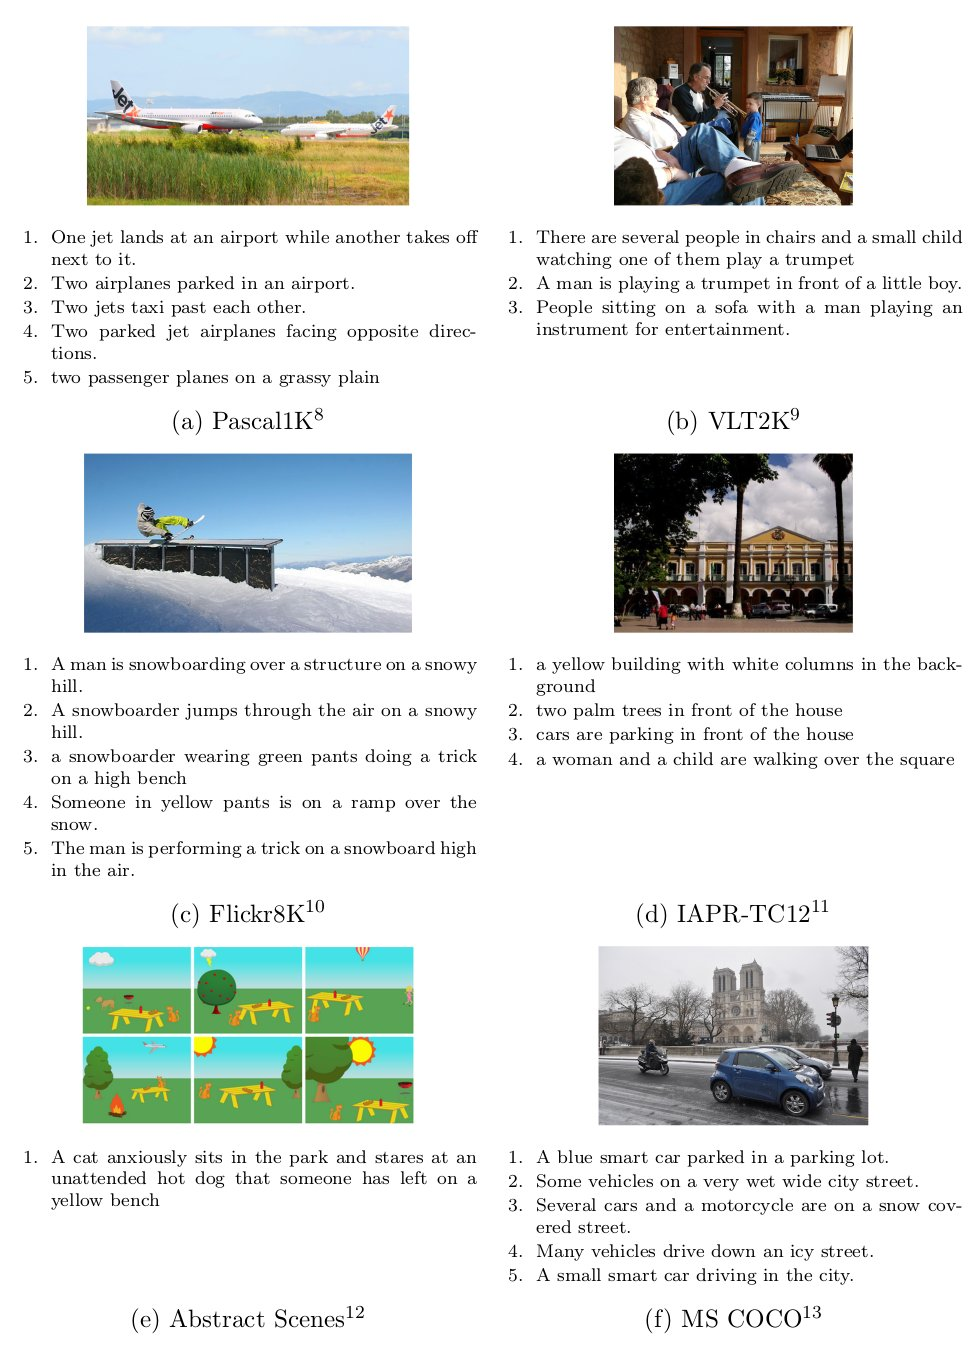
\includegraphics[scale=0.45]{images/ch2/image-caption-examples.jpg}
	\caption{Examples of images and their descriptions across various benchmark datasets}
	\label{fig:samples}
\end{figure}

\subsubsection{Other datasets}

This subsection summarizes other datasets that, in spite of being less popular that the ones already presented,  are to a certain extent relevant to the problem at hand.

\begin{itemize}
\item The Attribute Discovery dataset \citep{Berg2010} was collected using automatic dataset construction techniques that exploit the connection between text and images. This dataset consists of 4 broad shopping categories (bags, earrings, ties, and shoes). The data set was collected from \textit{like.com} and includes both images and associated textual descriptions.
\item The \textbf{MIT-Adobe FiveK} \citep{Bychkovsky2011} dataset consists of 5K images containing a diverse set of scenes, subjects, and lighting conditions. These images are mainly about people, nature, and man-made objects.
\item The \textbf{NYU-v2} dataset \citep{Silberman2012} is a more specialized dataset containing 1.5K RGBD images capturing 464 diverse indoor scenes, with detailed annotations. The particularity of this dataset is its focus on 3D segmentation. It has been augmented with five descriptions per image by \citet{Lin2015} for image description tasks.
\item The \textbf{SUN Attribute} database \citep{Patterson2014} provides around 15K  images from 707 scene categories. It was derived from the SUN categorical database using crowdsourcing to annotate images with attributes. Previously, crowdsourced human studies were preformed to find a taxonomy of 102 discriminative attributes related to varied aspects, such as materials, surface properties, lighting, affordances, and spatial layout.
\item The \textbf{FlickrStyle10k} dataset has 10K Flickr images with stylized captions. The training data consists of 7K images. The validation and test data consists of 2,000 and 1,000 images respectively. Each image contains romantic, humorous, and factual captions.
\item  The \textbf{Stock3M} dataset \citep{Wang2017} has more than 3M images uploaded by the users of a stock image website. Each image is associated with one caption that is provided by the photo uploader. The captions are much shorter than those found on the MSCOCO dataset, but are claimed to be more natural, with a larger vocabulary and image content variety.
\item The \textbf{VQA} (Visual Question Answering) dataset is intended to support a variation of the image description problem called \textit{visual question answering}: given an image and a natural language question about the image, the task is to provide an accurate natural language answer \citep{Antol2015}. To that aim, the dataset contains 50K abstract scenes using clip-art style graphics. It includes 20 paperdoll human models spanning genders, races, and ages with 8 different expressions, over 100 objects and 31 animals in various poses. The images are completed with five captions per image, as well as diverse questions and answers.
\end{itemize}

\subsection{Evaluation metrics}\label{sec:metrics}

Evaluating Natural Language Generation (NLG) systems is a fundamentally difficult task \citep{Reiter2009}, so that it has become a research problem itself. However, we will simply summarize the metrics commonly used for evaluating the quality of image descriptions generated automatically.

\subsubsection{Human judgement}

A common way to assess the quality of automatically generated texts is the subjective evaluation by human judges. Automatically produced text is usually judged in terms of syntactical correctness (grammar compliance) and semantic correctness (relevance of the content). Another dimension of interest is the fluency of the text, especially when a surface realization technique is involved in the generation process. Image descriptions generated automatically can be evaluated using the same techniques that are common in other NLG tasks, an very particularly in machine translation (MT) tasks. In this case, judges get both the image and the generated description for the evaluation task. Subjective human evaluations of machine generated image descriptions are often performed on the Amazon Mechanical Turk by means of Likert-scale questions. Some examples of these kind of questions are:

\begin{itemize}
\item The description accurately describes the image
\item The description is grammatically correct
\item The description has no incorrect information
\item The description is relevant for this image
\item The description is human like
\end{itemize}

\subsubsection{Automatic evaluation metrics}

Since human evaluation requires large amounts of non-reusable human effort, it is difficult to scale up. Furthermore, human judgement is inherently subjective, which makes it suffer from user variances. To avoid these pitfalls, automated metrics have been created with different properties. Below follows a short review of the most common metrics used for evaluating machine-generated image descriptions.

Classical \textbf{information retrieval metrics}, like the \textit{median rank} (mRank) and the \textit{precision and recall at k} (S@k, R@K) have been included quite often to evaluate the descriptions returned by image captioning methods, particularly with for methods that adopt an information retrieval approach, although they are not considered the most appropriate metric for this task.

IBM's \textbf{BLEU} (Bilingual Evaluation Understudy) \citep{Papineni2002} is a familiy of metrics conceived to substitute human judges in the evaluation of MT tasks, so besides being quick, inexpensive and language independent, it was designed to show good correlation with human judgement. This family of metrics use a weighted average of variable length phrase matches against the reference translations written by humans to measure their closeness. BLEU starts with a baseline metric from which a number of metrics are derived for different n-gram sizes: BLEU-1 compares the candidate sentence with sentences in unigram, BLEU-2 compares the candidate sentence with sentences in bigram, and so on, until BELU-4, which obtains the best correlation with human judgements While unigram scores account for the adequacy, higher n-gram scroes account for fluency. BLEU is popular because was it was the first metric popularized for MT tasks, long before the research on automatic image generation field took off. Although BLEU shows a reasonable correlation with human judgements it seems to work well only when the generated text is sort  \citep{Callison-Burch2006}, and it may even occur that an increase in BLEU score did not corresponds to an increase of quality \citep{Lin2004b}.

\textbf{ROUGE} (Recall-Oriented Understudy for Gisting Evaluation) \citep{Lin2004a} is a set of metrics introduced as an alternative to BLEU to work with larger texts, like text summaries. This metric employs the longest common subsequence between a candidate sentence and a set of reference sentences to measure their similarity at sentence-level. The longest common subsequence between two sentences only requires in-sequence word matches, and the matched words are not necessarily consecutive. Determination of the longest common subsequence is achieved by using dynamic programming. Different versions of ROUGE exist for different tasks: ROUGE-1 and ROUGE-W are appropriate for single document evaluation whereas ROUGE-2 and ROUGE-SU4 have good performance for short summaries. 

\textbf{METEOR} (Metric for Evaluation of Translation with Explicit ORdering) \citep{Banerjee2005} is another metric originally conceived to evaluate MT tasks. It is based on a generalized concept of unigram matching between the machine- produced translation and human-produced reference translations. Unigrams can be matched based on their surface forms, stemmed forms, and meanings. It first performs generalized unigram matches between a candidate sentence and a human-written reference sentence, and then computes a score based on the matching results. The score computation involves precision, recall and alignments of the matched elements, and in the case of multiple reference sentences, the best score among all the possible matches is taken as the final evaluation score. METEOR achieves better correlation at the sentence or the segment levels. There exists a \textit{Universal} version of this metric supporting many languages, like Russian and Hindi \citet{Denkowski2014}.

\textbf{CIDEr} (Consensus-based Image Description Evaluation) \citep{Vedantam2015} adopts a novel paradigm which is based on human consensus, and was designed specifically to evaluate image description tasks instead of MT tasks. This metric measures the similarity of an automatically generated sentence to the majority --consensus-- of ground-truth sentences (image descriptions) written by humans. It works by encoding the frequency of the n-grams in the candidate sentence that appear in the reference sentences using a Term Frequency Inverse Document Frequency (TF-IDF) weighting for each n-gram. While most existing datasets have only five captions per image, which the authors consider is not enough to use human consensus, therefore they also created two new datasets with 50 human-generated sentences per image: \textbf{Pascal-50S} and \textbf{Abstract-50S}, which uses the 1000 images from the Pascal1K, and 500 random images from the Abstract Scene dataset, respectively. A version of CIDEr named \textbf{CIDEr-D} is available as a part of the MSCOCO evaluation server to enable systematic evaluation and benchmarking.

\textbf{SPICE} (Semantic Propositional Image Caption Evaluation) \citep{Anderson2016} is a new evaluation metric for image descriptions based on a graph-based semantic representation of images called scene-graph \citep{Johnson2015, Schuster2015}. This graph can extract the information of different objects, attributes and their relationships from the image descriptions, and is based on the assumption than semantic propositional content is an important component of human caption evaluation. Extensive evaluations across a range of models and datasets indicate that SPICE captures human judgments over model-generated captions better than other automatic metrics. Furthermore, SPICE can answer questions such as which caption-generator best understands colors? and can caption-generators count?

\textbf{SPIDEr} \cite{Liu2017_PG} has been proposed recently to overcome some of the problems attributed to existing metrics by combining the properties of two of them: CIDEr and SPICE. This combination is achieved by means of a policy gradient (PG) method that directly optimizes a linear combination of SPICE and CIDEr (hence the name SPIDEr). SPICE score ensures semantic faithfulness of generated sentences, while CIDEr score guarantees that these descriptions are syntactically fluent.

\citep{Sharif2018} explore a learning-based approach to combine various metrics and report on their results. The idea behind this metric is the same behind SPIDEr: while some metrics tend to focus on the lexical and syntactical correctness (BLEU, ROUGE, CIDEr), other metrics tend to focus on the semantic relevance (SPICE). Therefore, combining the linguistic properties of various metrics should help achieve a better assessment of the quality of image description. Experimental results show improvements over other metrics in terms of correlation and accuracy on the Pascal-50S dataset.

\subsection{Summary of methods, datasets, metrics and benchmark results}\label{sec:summary_and_comparison}

This subsection summarises all the published research covered in this survey. We begin with an extended overview of the reviewed methods for image captioning that use deep learning techniques. We already presented an overview of methods in \cref{tab:overview}, but this time we include additional information to classify and characterize the methods. This information is described below, and it is presented in \cref{tab:classification}.

\begin{itemize}
\item The \textbf{network architecture} used to encode images. All methods use convolutional neural networks (CNN), but they differ in the specific network architecture, like VGG, Inception or ResNet, among others.
\item The kind of network used to learn the \textbf{language model}, typically some form of LSTM, but also other RNN and other models.
\item A classification of the method across multiple dimensions.
    \begin{itemize}
    \item \textbf{Visual Space (VS}) vs \textbf{Multimodal Space (MS}): Most methods model the image in the visual space, but some methods learn a combined visual and language space (see \cref{subsec:multimodal-learning})
    \item \textbf{Supervised Learning (SL}) vs \textbf{Other Deep Learning (ODL}). Although most methods use supervised learning, in some cases a form of semisupervised or unsupervised learning is employed (eg. generative adversarial networks (GAN) and reinforcement learning (RL)).
    \item \textbf{Whole Scene (WS}) vs \textbf{Dense Captioning (DC}): Most methods encode and describe images treated as a whole, but some approaches also detect regions in the image and generate descriptions for those regions.
    \item \textbf{Encode-Decoder (EDA}) vs \textbf{Compositional Architecture (CA}): many approaches adopt and encode-decoder architecture (see \cref{subsec:encoder-decoder_framework}), while only a few approaches adopt a compositional architecture (see \cref{subsec:compositional_architectures}).
    \end{itemize}
\item In addition to the above dimensions, some methods are annotated with extra descriptors to further characterize the image captioning methods:
    \begin{itemize}
    \item \textbf{Attention-Based (AB}) refers to methods that can dynamically focus on various parts of the image while the language descriptions are generated (see \cref{sec:attention-guided_models}).
    \item \textbf{Semantic Concept-Based (SCB}) methods selectively attend to a set of semantic concepts extracted from the image, so these methods apply a very specific form of attention mechanism.
    \item \textbf{Novel Object (NOB}) is used to characterize those methods that are able to describe objects that were not learned, that is, objects that were not included in the training dataset (see \cref{sec:novel_objects}).
    \item \textbf{Stylized Captions (SC)} refers to the use of styles  (eg. romantic, humorous) to generate more attractive captions. 
    \end{itemize}
\end{itemize}

Other acronyms used in this classification are:
\begin{itemize}
\item LBL: Log-Bilinear Language Model. It is a neural language model that operates on a feature vector representation of words. Word embeddings are computed using a feedforward neural network. Then, the probability of the next word is computed given the previous words (context) (see \citep{Mnih2007} for details).
\item SC-NLM: Structure-Content Neural Language Model. It is a multimodal neural language model proposed by \citep{Kiros2014_VS}
\item DTR: Dependency Tree Relations. Structure that represents all sentence relationships uniformly as typed dependency relations, that is, as triples of a relation between pairs of words (see \citep{DeMarneffe2006}).
\item MELM: Maximum Entropy Language Model. Model that predicts next word in a sentence based on the principle of maximum entropy (see \citep{Berger1996} for details).
\item HM-LSTM: Hierarchical Multimodal LSTM. Variation of the LSTM architecture proposed by \citet{Niu2017}
\item LCNN: Language CNN. Refers to the use of convolutional neural networks to represent language models \footnote{The use of CNNs for sentence modeling traces back to \citet{Collobert2008}. The ability of CNNs to create informative latent semantic representations of sentences for downstream tasks  \citet{Collobert2011,Kalchbrenner2014,Kim2014} led to a huge proliferation of CNN-based networks applied to NLP tasks.}. 
\end{itemize}

Note: In the classification presented in \cref{tab:classification}, we have omitted various methods described in the earlier works section (\cref{subsec:earlier_deep-learning_models}) that do not fit in the proposed dimensions. These methods are \citet{Socher2014, Lebret2015a, Lebret2015b, Yagcioglu2015}.

\begin{longtable}{ p{.30\textwidth} p{.20\textwidth} p{.20\textwidth} p{.30\textwidth}}
    \caption{Classification of deep-learning methods}\\
    \toprule
    Publication &  Image Encoder & Language Model & Category\endhead
    \midrule
    \citet{Karpathy2014} & AlexNet & DTR & MS,SL,WS,EDA \\
    \citet{Kiros2014_VS} & AlexNet & LBL & MS,SL,WS,EDA \\
    \citet{Kiros2014_LBL} & AlexNet, VGG & LSTM,SC-NLM & MS,SL,WS,EDA \\
    \citet{Mao2014} & AlexNet & RNN & MS,SL,WS \\
    \citet{Chen2015} & VGG & RNN & VS,SL,WS,EDA \\
    \citet{Donahue2015} & Caffe & LSTM & VS,SL,WS,EDA\\
    \citet{Devlin2015} & VGG & MELM & MS,SL,SL,WS,EDA\\
    \citet{Fang2015} & AlexNet,VGG & MELM & VS,SL,WS,EDA \\
    \citet{Jia2015} & VGG & LSTM & VS,SL,WS,CA, SCB \\
    \citet{Karpathy2015} & VGG & RNN & MS,SL,WS,EDA \\
    \citet{Ma2015} & VGG & LCNN & MS,SL,WS,EDA \\
    \citet{Mao2015_mRNN} & AlexNet,VGG & RNN & MS,SL,WS\\
    \citet{Vinyals2015} & Inception-V1 & LSTM & VS,SL,WS,EDA\\
    \citet{Xu2015} & AlexNet & LSTM & VS,SL,WS,EDA,AB\\
    \citet{Hendricks2016} & VGG & LSTM & VS,SL,WS,CA,NOB\\
    \citet{Johnson2016} & VGG & LSTM & VS,SL,DC,EDA\\
    \citet{Ma2016} & AlexNet & LSTM & VS,SL,WS,CA\\
    \citet{Mao2016} & AlexNet,VGG & LSTM & VS,SL,WS,EDA\\
    \citet{Mathews2016} & Inception-V1 & LSTM & VS,SL,WS,EDA,SC\\
    \citet{Sugano2016} & VGG & LSTM & VS,SL,WS,EDA,AB\\
    \citet{Tran2016} & ResNet & MELM & VS,SL,WS,CA\\
    \citet{Wang2016_Parallel} & VGG & LSTM & VS,SL,WS,CA\\
    \citet{Wu2016} & VGG & LSTM & VS,SL,WS,EDA,SCB\\
    \citet{Yang2016_RevNet} & VGG & LSTM & VS,SL,DC,EDA,AB\\
    \citet{You2016} & Inception-V1 & RNN & VS,SL,WS,EDA,SCB\\
    \citet{Chen2017_SCA} & VGG,ResNet & LSTM & VS,SL,EDA,AB\\
    \citet{Dai2017_CGAN} & VGG & LSTM & VS,ODL,WS,EDA\\
    \citet{Fu2017} & VGG & LSTM & VS,SL,WS,EDA,AB\\
    \citet{Gan2017_Style} & ResNet & LSTM & VS,SL,WS,EDA,SC\\
    \citet{Gan2017_SCN} & ResNet & LSTM & VS,SL,WS,CA,SCB\\
    \citet{Gu2017} & VGG & LCNN,LSTM & VS,SL,WS,EDA\\
    \citet{Liu2017_SAM} & VGG & LSTM & VS,SL,WS,EDA,AB\\
    \citet{Liu2017_PG} & Inception-V3 & LSTM & VS,RL,WS,EDA\\
    \citet{Liu2017_MAT} & CNN+LSTM & LSTM & VS,SL,DC,EDA,AB\\
    \citet{Lu2017} & ResNet & LSTM & VS,SL,WS,EDA,AB\\
    \citet{Niu2017} & AlexNet & HM-LSTM & MS,SL,DC,EDA\\
    \citet{Park2017} & ResNet & LSTM & VS,SL,WS,EDA,AB\\
    \citet{Pedersoli2017} & VGG & RNN & VS,SL,WS,EDA,AB\\
    \citet{Ren2017} & VGG & LSTM & VS,ODL,WS,EDA\\
    \citet{Rennie2017} & ResNet & LSTM & VS,ODL,WS,EDA\\
    \citet{Shetty2017} & Inception-V1 & LSTM & VS,ODL,WS,EDA\\
    \citet{Tavakoliy2017} & VGG & LSTM & VS,SL,WS,EDA,AB\\
    \citet{Venugopalan2017} & VGG & LSTM & VS,SL,WS,CA,NOB\\
    \citet{Wang2017} & ResNet & LSTM & VS,SL,WS,EDA\\
    \citet{Yang2017} & VGG & LSTM & VS,SL,DC,EDA,AB\\
    \citet{Yao2017_Attr} & Inception-V1 & LSTM & VS,SL,WS,EDA,SCB\\
    \citet{Yao2017_NOB} & VGG & LSTM & VS,SL,WS,CA,NOB\\
    \citet{Zhang2017} & Inception-V3 & LSTM & VS,RL,WS,EDA\\
    \citet{Aneja2018} & VGG & LCNN & VS,SL,WS,EDA\\
    \citet{Jiang2018} & Inception-V3 & LSTM & VS,SL,WS,EDA,AB\\
    \citet{Khademi2018} & VGG,ResNet & Grid LSTM & VS,SL,DC,EDA,AB\\
    \citet{Li2018_VS-LSTM} & Faster R-CNN & LSTM & VS,RL,DC,EDA,SCB\\
    \citet{Wang2018} & VGG & LCNN & VS,SL,WS,EDA\\
    \bottomrule
\label{tab:classification}
\end{longtable}

% Skipped Chen2017_RLSTM, Feng2018,Gu2018, Li2018_CAL

Next, we present two tables that enumerate the datasets and evaluation metrics reported in each of the publications. Due to the large number of publications, we have divided them in two groups, one devoted to those proposals that are not based on neural networks, and another one with those proposals based on neural networks and deep learning.

\clearpage
\begin{table}[ht]
\caption{Summary of non neural methods, datasets and evaluation metrics.}
\begin{tabular}{p{.30\textwidth} p{.30\textwidth} p{.40\textwidth}}
    \toprule
    Publication &  Datasets & Evaluation Metrics\\
    \midrule
    \citet{Farhadi2010} & Pascal1K & BLEU \\
    \citet{Kulkarni2011} & Pascal1K & Human, BLEU \\
    \citet{Li2011} & Pascal1K & Human, BLEU \\
    \citet{Ordonez2011} & SBU &  \\
    \citet{Yang2011} & Pascal1K & BLEU, ROUGE, METEOR \\
    \citet{Gupta2012} & Pascal1K & Human, BLEU, ROUGE \\
    \citet{Kuznetsova2012} & SBU & Human, BLEU \\
    \citet{Mitchell2012} & Pascal1K & Human \\
    \citet{Elliott2013} & VLT2K & Human, BLEU \\
    \citet{Hodosh2013b} & Pascal1K, Flickr8K & Human, BLEU, ROUGE, mRank, R@k \\
    \citet{Gong2014} & SBU, Flickr30K & R@k \\
    \citet{Kuznetsova2014} & SBU & Human, BLEU, METEOR \\
    \citet{Patterson2014} & SBU & BLEU \\
    \citet{Socher2014} & Pascal1K & mRank, R@k \\
    \citet{Verma2014} & IAPR, SBU, Pascal1K & BLEU, ROUGE, R@k \\
    \citet{Yatskar2014} & Own data & Human, BLEU \\
    \citet{Elliott2015} & VLT2K, Pascal1K & BLEU, METEOR \\
    \citet{Lebret2015a}\textsuperscript{*} & Flickr30K, COCO & BLEU, R@k \\
    \citet{Lebret2015b}\textsuperscript{*} & COCO & BLEU \\
    \citet{MateosOrtiz2015} & Abstract Scenes & Human, BLEU \\
    \citet{Ushiku2015} & Pascal1K, IAPR, SBU, COCO & BLEU \\
    \bottomrule
\end{tabular}
\label{tab:methods_datasets_metrics}
\end{table}

\textsuperscript{*} Note that \citep{Lebret2015a, Lebret2015b} do not use neural nets as part of their learning method, but they use a pretrained CNN for the representation of images, so they are in the frontier of both worlds. For this reason we have included them in both summary tables, the first one, devoted to non-neural methods, as well as the second one, dedicated to neural-based methods. 

\begin{longtable}{ p{.30\textwidth} p{.30\textwidth} p{.40\textwidth} }
    \caption{Summary of neural methods, datasets and metrics}\\
    \toprule
    Publication &  Datasets & Evaluation Metrics\endhead
    \midrule
    \citet{Karpathy2014} & Flickr8K/30K, COCO & BLEU, METEOR, CIDEr \\
    \citet{Kiros2014_VS} & IAPTR, Attribute Descriptions & BLEU, PPLX \\
    \citet{Kiros2014_LBL} & Flickr8K/30K & R@k, mRank \\
    \citet{Mao2014} & IAPTR, Flickr8K/30K & BLEU, mRank, R@k \\
    \citet{Chen2015} & Pascal1K, Flickr8K/30K, COCO & BLEU, METEOR, CIDEr, mRank, R@k \\
    \citet{Donahue2015} & Flickr30K, COCO & Human, BLEU, mRank, R@k \\
    \citet{Devlin2015} & COCO & BLEU, METEOR \\
    \citet{Fang2015} & Pascal1K, COCO & Human, BLEU, METEOR, PPLX \\
    \citet{Jia2015} & Flickr8K/30K, COCO & BLEU, METEOR, CIDEr \\
    \citet{Karpathy2015} & Flickr8K/30K, COCO & BLEU, METEOR, CIDEr, mRank, R@k \\
    \citet{Lebret2015a} & Flickr30K, COCO & BLEU, R@k \\
    \citet{Lebret2015b} & COCO & BLEU \\
    \citet{Ma2015} & Flickr8K/30K & mRank, R@k \\
    \citet{Mao2015_mRNN} & IAPR, Flickr30K, COCO & BLEU, mRank, R@k \\
    \citet{Vinyals2015} & Pascal1K, SBU, Flickr30K, COCO & Human, BLEU, METEOR, CIDEr, mRank, R@k \\
    \citet{Xu2015} & Flickr8K/30K, COCO & BLEU, METEOR \\
    \citet{Yagcioglu2015} & Flickr8K/30K, COCO & Human, BLEU, METEOR, CIDEr \\
    \citet{Hendricks2016} & COCO, ImageNet & BLEU, METEOR \\
    \citet{Johnson2016} & Visual Genome & METEOR, AP, IoU \\
    \citet{Ma2016} & Flickr8K, UIUC & BLEU, R@k \\
    \citet{Mao2016} & ReferIt & BLEU, METEOR, CIDEr \\
    \citet{Mathews2016} & COCO, SentiCap & BLEU, METEOR, ROUGE, CIDEr \\
    \citet{Sugano2016} & COCO & BLEU, METEOR, ROUGE, CIDEr \\
    \citet{Tran2016} & COCO, MIT-Adobe, Instagram &  Human\\
    \citet{Wang2016_Parallel} & Flickr8K & BLEU, METEOR, PPLX \\
    \citet{Yang2016_RevNet} & COCO & BLEU, METEOR, CIDEr \\
    \citet{You2016} & Flickr30K, COCO & BLEU, METEOR, ROUGE, CIDEr \\
    \citet{Chen2017_SCA} & Flickr8K/30K, COCO & BLEU, METEOR, ROUGE, CIDEr \\
    \citet{Dai2017_CGAN} & Flickr30K, COCO & BLEU, METEOR \\
    \citet{Fu2017} & Flickr8K/30K, COCO & BLEU, METEOR, ROUGE, CIDEr \\
    \citet{Gan2017_Style} & FlickrStyle10K & BLEU, METEOR, ROUGE, CIDEr \\
    \citet{Gan2017_SCN} & Flickr30K, COCO &  BLEU, METEOR, CIDEr \\
    \citet{Gu2017} & Flickr30K, COCO & BLEU, METEOR, CIDEr, SPICE \\
    \citet{Liu2017_SAM} & Flickr30K, COCO & BLEU, METEOR \\
    \citet{Liu2017_PG} & COCO & Human, BLEU, METEOR, ROUGE, CIDEr, SPIDEr \\
    \citet{Lu2017} & Flickr30K, COCO & BLEU, METEOR, CIDEr \\
    \citet{Park2017} & Instagram & BLEU, METEOR, ROUGE, CIDEr \\
    \citet{Pedersoli2017} & COCO & BLEU, METEOR, CIDEr \\
    \citet{Ren2017} & COCO & BLEU, METEOR, ROUGE, CIDEr \\
    \citet{Rennie2017} & COCO & BLEU, METEOR, CIDEr, SPICE \\
    \citet{Shetty2017} & COCO & BLEU, METEOR, SPICE \\
    \citet{Tavakoliy2017} & COCO, Pascal 50S & BLEU, METEOR, ROUGE, CIDEr \\
    \citet{Venugopalan2017} & COCO, ImageNet & METEOR \\
    \citet{Wang2017} & COCO, Stock3M & METEOR, ROUGE, CIDEr, SPICE \\
    \citet{Yang2017} & VisualGenome & METEOR, AP, IoU \\
    \citet{Yao2017_Attr} & COCO & BLEU, METEOR, ROUGE, CIDEr \\
    \citet{Yao2017_NOB} & COCO, ImageNet & METEOR \\
    \citet{Zhang2017} & COCO & BLEU, METEOR, ROUGE, CIDEr \\
    \citet{Aneja2018} & COCO & BLEU, METEOR, ROUGE, CIDEr \\
    \citet{Jiang2018} & COCO & BLEU, METEOR, ROUGE, CIDEr\\
    \citet{Khademi2018} & COCO & BLEU, METEOR, ROUGE, CIDEr\\
    \citet{Wang2018} & COCO & BLEU, METEOR, ROUGE, CIDEr \\
    \bottomrule
\label{tab:nn_methods_datasets_metrics}
\end{longtable}

Finally, we conclude this section, and the review, with a  comparison of methods across the most popular benchmark datasets and evaluation metrics, that is: Flickr30K and MSCOCO datasets, and the BLUE, ROUGE, METEOR and CIDEr metrics. This is not an exhaustive review, but we have included the most cited ones that include comparable results.

\cref{tab:benchmarks_flickr30k} compares results by various methods on the Flickr30K dataset. In this table Bn, M, and C refer, respectively, to BLEU-n, METEOR and CIDEr scores.

\clearpage
\begin{table}[ht]
\caption{Comparison of methods on the Flickr30K dataset}
\begin{tabular}{lcrrrrr}
    \toprule
    Method	&	B1	&	B2	&	B3	&	B4	&	M	&	C	\\
    \midrule
    \citet{Kiros2014_LBL}	&	60	&	38	&	25.4	&	17.1	&	16.9	&		\\
    \citet{Chen2015}	&		&		&		&	12.6	&	16.4	&		\\
    \citet{Donahue2015}	&	58.7	&	39.1	&	25.1	&	16.5	&		&		\\
    \citet{Jia2015}	&	64.6	&	44.6	&	30.5	&	20.6	&	17.9	&		\\
    \citet{Karpathy2015}	&	57.3	&	36.9	&	24	&	15.7	&		&		\\
    \citet{Mao2015_mRNN}	&	60	&	41	&	28	&	19	&		&		\\
    \citet{Vinyals2015}	&	66.3	&	42.3	&	27.7	&		&		&		\\
    \citet{Xu2015} Soft	&	66.7	&	43.4	&	28.8	&	19.1	&	18.49	&		\\
    \citet{Xu2015} Hard	&	66.9	&	43.9	&	29.6	&	19	&	18.5	&		\\
    \citet{Oruganti2016}	&	58.9	&	40	&	26.6	&	17.7	&	17.8	&		\\
    \citet{Wu2016}	&	73	&	55	&	40	&	28	&		&		\\
    \citet{You2016}	&	64.7	&	46	&	32.4	&	23	&	18.9	&		\\
    \citet{Chen2017_SCA}	&	66.2	&	46.8	&	32.5	&	22.3	&	19.5	&	44.7	\\
    \citet{Gan2017_SCN}	&	74.7	&	55.2	&	40.3	&	28.8	&		&		\\
    \citet{Gu2017}	&	73.8	&	56.3	&	41.9	&	30.7	&	20.6	&		\\
    \citet{Fu2017}	&	64.9	&	46.2	&	32.4	&	22.4	&	19.4	&		\\
    \citet{Lu2017}	&	67.7	&	49.4	&	35.4	&	25.1	&	20.4	&	53.1	\\
    \citet{Li2018_VS-LSTM}	&	\textbf{75.5}	&	\textbf{57.1}	&	\textbf{42.9}	&	\textbf{31.7}	&	\textbf{22.9}	&	\textbf{71.5}	\\
    \citet{Wang2018} 	&	57.7	&	40.1	&	27.6	&	19	&	18.4	&	35.2	\\
    \citet{Wang2018} Hier	&	60.7	&	42.5	&	29.2	&	19.9	&	19.1	&	39.5	\\
    \bottomrule
\end{tabular}
\label{tab:benchmarks_flickr30k}
\end{table}

\cref{tab:benchmarks_mscoco} compares results on the MSCOCO dataset. In this table Bn, M, R and C refer, respectively, to BLEU-n, METEOR, ROUGE-L and CIDEr scores. Scores in bold and italics indicate the best and the second best results in a given metric, respectively. Methods marked with * are ensemble methods.

\clearpage
\begin{table}[ht]
\caption{Comparison of methods on the MSCOCO dataset}
\begin{tabular}{lcrrrrrr}
    \toprule
    Method	&	B1	&	B2	&	B3	&	B4	&	M	&   R   &	C \\
    \midrule
    \citet{Kiros2014_LBL}	&	70.8	&	48.9	&	34.4	&	24.3	&	20.03	&		&		\\
    \citet{Chen2015}	&		&		&		&	19	&	20.4	&		&		\\
    \citet{Donahue2015}	&	66.9	&	48.9	&	34.9	&	24.9	&		&		&		\\
    \citet{Fang2015}	&		&		&		&	25.7	&	23.6	&		&		\\
    \citet{Jia2015}	&	67	&	49.1	&	35.8	&	26.4	&	22.7	&		&	81.3	\\
    \citet{Karpathy2015}	&	62.5	&	45	&	32.1	&	23	&	19.5	&		&	66	\\
    \citet{Mao2015_mRNN}	&	66.8	&	48.8	&	34.2	&	23.9	&	22.1	&	48.9	&	72.9	\\
    \citet{Vinyals2015}	&	66.6	&	46.1	&	32.9	&	24.6	&		&		&	85.5	\\
    \citet{Xu2015} Soft	&	70.7	&	49.2	&	34.4	&	24.3	&	23.9	&		&		\\
    \citet{Xu2015} Hard	&	71.8	&	50.4	&	35.7	&	25	&	23	&		&		\\
    \citet{Oruganti2016}	&	70.2	&	52.8	&	38.3	&	27.6	&	22.5	&		&		\\
    \citet{Wu2016}	&	74	&	56	&	42	&	31	&	26	&		&	94	\\
    \citet{Yang2016_RevNet}	&	73.8	&		&		&	29	&	23.7	&		&	88.6	\\
    \citet{You2016}	&	70.9	&	53.7	&	40.2	&	30.4	&	24.3	&		&		\\
    \citet{Chen2017_SCA}	&	71.9	&	54.8	&	41.1	&	31.1	&	25	&		&	95.2	\\
    \citet{Chen2017_RLSTM}	&	76.1	&	59.6	&	45	&	33.7	&	25.7	&	55	&	102.9	\\
    \citet{Fu2017}	&	72.4	&	55.5	&	41.8	&	31.3	&	24.8	&	53.2	&	95.5	\\
    \citet{Gan2017_SCN}	&	74.1	&	57.8	&	44.4	&	34.1	&	26.1	&		&	104.1	\\
    \citet{Gu2017}	&	72.3	&	55.3	&	41.3	&	30.6	&		&	25.2	&	98.9	\\
    \citet{Liu2017_MAT}	&	73.1	&	56.7	&	42.9	&	32.3	&	25.8	&		&	105.8	\\
    \citet{Lu2017}	&	74.2	&	58	&	43.9	&	33.2	&	26.6	&		&	108.5	\\
    \citet{Mun2017}	&	74.9	&	58.1	&	43.7	&	32.6	&	25.7	&		&	102.4	\\
    \citet{Ren2017}	&	71.3	&	53.9	&	40.3	&	30.4	&	25.1	&	52.5	&	93.7	\\
    \citet{Rennie2017} 	&		&		&		&	34.2	&	26.7	&	55.7	&	114	\\
    \citet{Rennie2017}*	&		&		&		&	35.4	&	27.1	&	56.6	&	117.5	\\
    \citet{Shetty2017}	&		&		&		&		&	27.2	&		&		\\
    \citet{Wang2017}	&	74.2	&	57.7	&	44	&	33.6	&	26.8	&	55.2	&	107.3	\\
    \citet{Yao2017_Attr}	&	73.4	&	56.7	&	43	&	32.6	&	25.4	&		&	100.2	\\
    \citet{Zhang2017}	&		&		&		&	34.4	&	26.7	&	55.8	&	116.2	\\
    \citet{Zhou2017}	&	71.6	&	54.5	&	40.5	&	30.1	&	24.7	&		&	97	\\
    \citet{Anderson2018_BUTD}	&	77.2	&		&		&	36.2	&	27	&	56.4	&	113.5	\\
    \citet{Anderson2018_BUTD}  opt	&	79.8	&		&		&	36.3	&	27.7	&	56.9	&	120.1	\\
    \citet{Aneja2018}	&	71.1	&	53.8	&	39.4	&	28.7	&	24.4	&	52.2	&	91.2	\\
    \citet{Gu2018}	&	78.6	&	62.5	&	47.9	&	36.1	&	27.4	&	56.9	&	120.4	\\
    \citet{Jiang2018}	&	75.1	&	59.2	&	45.8	&	35.3	&	26.7	&	55.5	&	107.8	\\
    \citet{Khademi2018}	&	76.2	&	60.1	&	45.1	&	35	&	27	&		&		\\
    \citet{Wang2018}	&	68.8	&	51.3	&	37	&	26.5	&	23.4	&	50.7	&	83.9	\\
    \citet{Wang2018} Hier	&	68.5	&	51.1	&	36.9	&	26.7	&	23.4	&	51	&	84.4	\\
    \bottomrule
\end{tabular}
\label{tab:benchmarks_mscoco}
\end{table}

% TODO

% Optionally add scores from MSCOCO leaderboard

% Comments on which kind of approaches get better results, and comment about the impact of fine tuning vs model concept in the final scores
% See https://news.ycombinator.com/item?id=10611639
\chapter{Scope}
\label{ch:scope}

This chapter constitutes a preparatory step before describing the model in the next chapter. On the one hand, this chapter lays out the scope of the project and justifies the main design decisions taken for developing a system. In the other hand, it presents the architectural framework adopted in our system and provides some theoretical background.

\section{Scope}\label{sec:scope}

Before diving into the design of the system developed for this project, it seems convenient to delimit the scope of it as well as justify the design decisions taken. In particular, we have to decide on three main separated aspects:

\begin{enumerate}
\item To begin with, we should decide on the kind of architecture to design our system, which can further be divided into various finer details, like deciding the concrete models to use for each component of the architecture, whether to use transfer learning, and whether to use ensemble methods, among others.
\item Another decision of high importance if the dataset to use in order to train and evaluate our system. As a secondary decision, we should also decide which metrics to use for evaluating it.
\item Finally, we should decide on the specific experiments, which in turn will involve deciding on various hyper-parameters and configuration options that may be available in our model.
\end{enumerate}

Deciding on those three aspects should be conditioned by a combination of factors, from research considerations to hardware requirements and time constraints. This chapter will briefly discuss these aspects, and then we will conclude with the final decisions that define the scope of the system to be developed as part of this project.

\subsection{Research considerations}

As we have seen in our review of the state of the art (\cref{ch:state_of_the_art}), image captioning is a thrilling field of research that has seen tremendous advances in recent years, especially since neural networks and deep learning were applied to it. From the first neural model proposed by \citet{Kiros2014_LBL}, a myriad of different neural models have been proposed, usually combining a visual encoder and a text decoder. Although there are some exceptions, the majority of the models proposed so far use some form of Convolutional Neural Network (CNN) for the encoder, and some form of Recurrent Neural Network (RNN) for the decoder. Some models also use CNN for the decoder, and a few recent models include Generative Adversarial Networks (GAN) to achieve more varied and expressive captions. Most of the proposed models use some form of supervised learning, typically back-propagation, but there is a growing number of models that include reinforcement learning, and there have been some recent attempts to use also semi-supervised learning, and even unsupervised learning. 

Summing up, there are many options to choose from in order to develop our own image captioning system. If we look at the results obtained from these models in benchmark datasets, we can see various patterns and trends.

\begin{itemize}
\item First, end-to-end approaches based on the encoder-decoder framework prevail over compositional architectures.
\item Second, attention mechanisms have flourished and are a key component included in the vast majority of models, although they can adopt different forms.
\item Third, the addition of reinforcement learning is gaining a lot of momentum as a means to improve the quality of generated captions when considering language quality metrics such as CIDEr.
\item Fourth, models tend to increase in complexity by stacking more layers and including additional methods and forms of learning. Another aspect of this trend is the use of ensemble methods that combine various models together to produce the final result.
\end{itemize}

Besides the aforementioned trends and patterns, the study of the published research relative to image captioning reveals a 
high degree of alignment between this research and the more general research sequence-to-sequence (\textit{seq2seq}) learning and sequence translation problems. Therefore, it would be interesting to study current trends in \textit{seq2seq} research to anticipate the next advances in image captioning.

Indeed, neural image captioning systems adopted the encoder-decoder architecture used in sequence translation, with the particularity of using CNN for the encoder, but the decoder is an RNN as those used in seq2seq problems. Next, ResNet and Attention make its appearance and rapidly gained popularity, both in seq2seq learning and image captioning.

Attention-based networks are increasingly used by the big players in the IT world, including Google and Facebook. The main reason for this shift from simple RNN to attention-based architectures is because the former requires more resources to train and run than the latter. Therefore, we deem attention as a key ingredient to include in our own system.

\subsection{Hardware requirements and time constraints}

Although for some projects hardware and time may appear as two separate aspects to factor in, they are closely related when we are dealing with deep learning. That is because due to the vast size of some datasets, training some systems may require either fabulous hardware resources or incredibly long periods, and even a combination of both.

For this project we have to deal with a combination of both little time and limited hardware resources, so we have to limit the scope of our project to something manageable.

At the beginning of this project, we had at our disposal a computer equipped with an NVIDIA GTX 1070 GPU supporting CUDA, which is a must-have for any deep learning project beyond toy examples.

After doing some preliminary experiments we realized that with the hardware at hand, it was going to be unfeasible to work with state of the art benchmark datasets such as MS COCO (not to mention the Conceptual Captions dataset, recently released by Google). Furthermore, we got serious problems when using the computer in interactive mode whilst training a deep learning model. 

One option was to conduct our experiments on a smaller, dataset such as the Flickr8K or perhaps the Flickr30K dataset, but there are quite outdated nowadays. Therefore, in order to work with larger datasets, I decided to invest in a new, more powerful GPU, and so I bought an NVIDIA GTX 20180 Ti. I got this GPU installed on the same computer, alongside the GTX 1070. As a result of the new configuration, the training times reduced considerably, and it became feasible to use the computer whilst training a model on the COCO dataset.

The most relevant specifications of the final hardware used to conduct the experiments as as follows:

\begin{itemize}
\item CPU: Intel Core i7-4790K (4 cores, 8 threads clocked @ 4 GHz)
\item RAM: 16GB DIMM DDR3 2400 (clocked @ 1333 MHz)
\item Storage: 2 x SSD Samsung 850 Evo 250GB
\item GPU-0: NVIDIA GTX 1070, 6GB RAM
\item GPU-1: NVIDIA RTX 2080 Ti, 11GB RAM
\end{itemize}

Note the two GPUs included in the system. The GTX 1070 is used as the rendering unit, for interactive tasks, while the RTX 2080 Ti is used as the main CUDA platform to carry on the data-intensive tasks required to train and evaluate our model on big datasets. With that hardware, we deem it possible to train models one the full COCO dataset in less than a week, depending on the concrete architecture of the net and different hyperparameters on the net, as well as some restrictions imposed on the training data, such as the size of the vocabulary, or the maximum caption length allowed.

\subsection{Software requirements}

With respect to the software requirements, from the very beginning of the project we  two general requirements were clear:
\begin{itemize}
    \item Using a language we are familiar with
    \item Using a popular framework with a big community 
\end{itemize}

The combination of the two requisites above led us to choose Python as the development language, and Keras with Tensorflow backend as the computational framework. 

However, in the end, we decided to take a little risk by using an alpha version of the \textbf{Keras-Tensorflow} API stack that has been released recently as part of the new \textbf{Tensorflow 2.0.0-alpha}.

\subsection{Summing up}

The study of published research resulted in the selection of an \textbf{encoder-decoder architecture with a soft attention mechanism} based on the model proposed by \citet{Xu2015}. 

However, there are so many options to choose from for the different components of our system, that we should limit those options to a few options.
\begin{itemize}
    \item \textbf{Encoder}: we aim at trying at least two different encoders, like the Inception-V3 network, and the NASNet.
    \item \textbf{Decoder}: for this component, the idea is to try both GRU and LSTM units. 
    \item \textbf{Attention} mechanism: we aim at trying the soft attention mechanism, which is easier to implement
\end{itemize}

Finally, if there is enough time we may try different hyper-parameters, such as the number of hidden units or units in the embedding layer. Other options to play with are the size of the vocabulary, but that is difficult to estimate at this stage of the project.

\section{The Encoder-Decoder architecture}\label{sec:encoder-decoder}

\subsection{From feature engineering to feature learning}

Machine learning algorithms take features as inputs and produce some output. How we represent features makes a huge difference in the performance of the learning algorithms.  Traditionally, approaches to machine learning require a strong \textbf{feature engineering} approach, meaning that the designer has to carefully choose features and their representation before feeding them into the algorithm. When facing complex problems like computer vision, this approach came up with sophisticated representations, such as HOG (Histogram of Oriented Gradients) for representing image features.

Due to such representations, there is a difference to be made between the \textit{raw inputs}, and the features which are input to the model. For example, in face recognition, the pixels of a picture are the raw input, while the HOG features of the image can be the actual input to the model.

Someone came up with the idea that we can use an algorithm to learn the feature representation itself, aptly called \textbf{feature learning}. Deep learning uses a neural network model to achieve this task. In point of fact, feature learning is accomplished by the first layers of a neural network, which map raw inputs to efficient feature representations. The last layers (typically fully connected layers) mix and match and combine these features to produce an output.

\subsection{The encoder-decoder architecture}

The \textbf{encoder-decoder architecture} explicitly aims to leverage this ability of neural networks to learn efficient representations. It is a neural network design pattern that consists of two main components, the \textit{encoder} and the \textit{decoder}.  The \textbf{encoder} maps raw inputs to feature representations, and these representations are then passed to the \textbf{decoder}, which has to produce an output. This is commonly referred to as the encoder-decoder framework, and its general architecture is shown in \cref{fig:encoder-decoder}

\begin{figure}[hpt]
    \centering
    \includesvg{images/ch3/encoder-decoder.svg}
    \caption{The encoder-decoder architecture.}
    \label{fig:encoder-decoder}
\end{figure}

Theoretically, encoder and decoder parts can be used independently of each other. For instance, an encoder RNN can be used to encode the features of an incoming email as a \textit{features vector}, which is then used as input to a Fully-Connected Layer (FCL) to predict whether the email is spam or not. However, neural encoder and decoders are often used in a tightly coupled manner, meaning that the system is trained as a whole. This approach, known as \textbf{end-to-end}, is been increasingly used due to a combination of good performance and less engineering effort.

The encoder-decoder architecture is enormously popular in the fields of computer vision and natural language processing and may adopt very different forms. In some cases, the same type of network is used for both the encoder and the encoder.

For example, \cref{fig:cnn-cnn} depicts an example of a pure convolutional encoder-decoder architecture (there is no fully connected layer). This model is used to perform semantic segmentation of an image. The left half of the network (the encoder) maps raw image pixels to a rich representation consisting of feature vectors. The right half of the network (the decoder) takes these features and upsamples them to produce a sparse feature map which is fed to a soft-max for pixel-wise classification.

\begin{figure}[hpt]
    \centering
    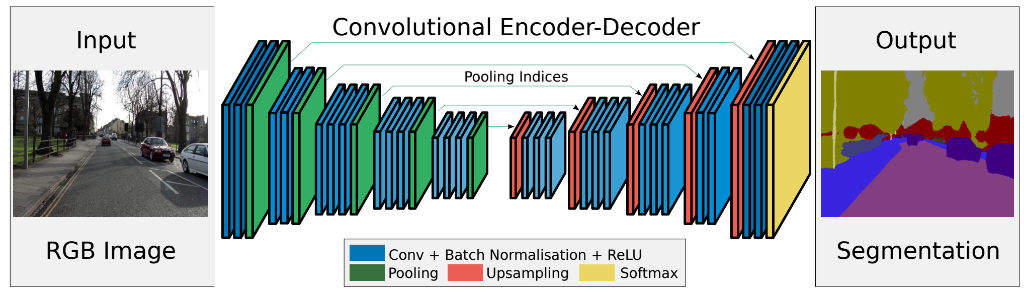
\includegraphics[scale=0.45]{images/ch3/cnn-cnn.png}
    \caption{Convolutional encoder-decoder for image segmentation in the SeqNet architecture \citep{Badrinarayanan2017}}
    \label{fig:cnn-cnn}
\end{figure}

Encoder-decoder networks based on RNN are very common in problems requiring \textit{sequence-to-sequence (seq2seq)} modeling, such as translation, summarising and question-answering. For example, \cref{fig:rnn-rnn} shows an example of a model used to generate automatic responses to incoming emails. The left half of the network encodes the email into a feature vector, and the right half of the network decodes the feature vector to produce word predictions. 

\begin{figure}[hpt]
    \centering
    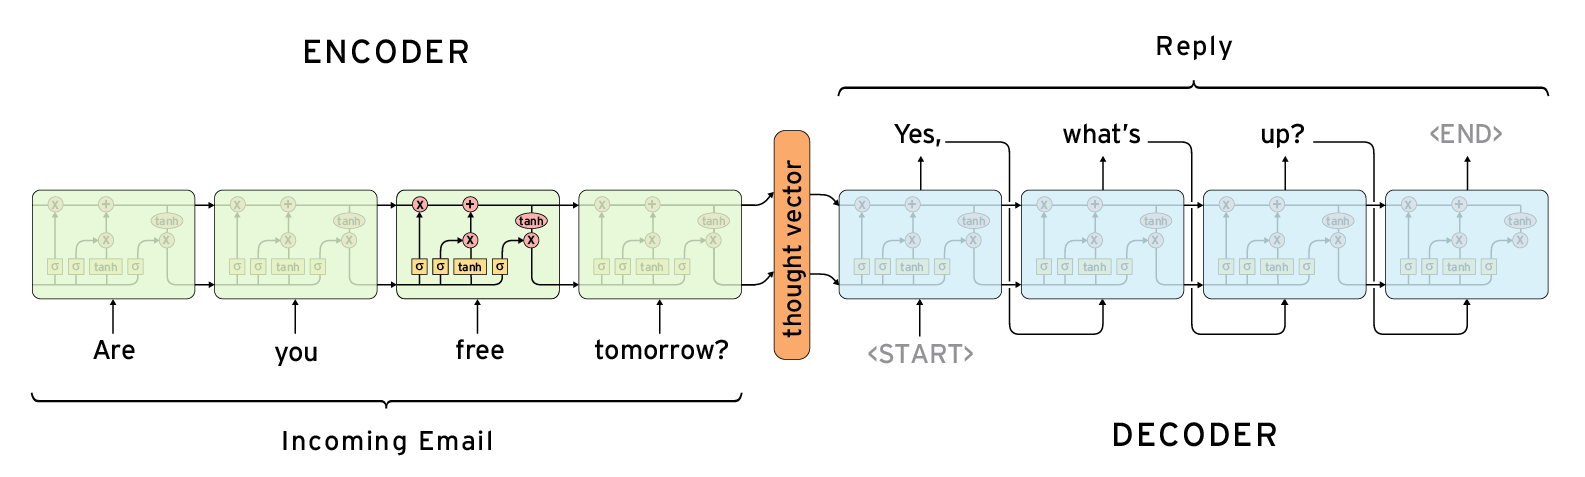
\includegraphics[scale=0.3]{images/ch3/rnn-rnn.png}
    \caption{Recurrent encoder-decoder for automated email answering. The model is given input a sentence and produces a response in the same language. Source: \href{https://ai.googleblog.com/2015/11/computer-respond-to-this-email.html}{Google AI Blog}}
    \label{fig:rnn-rnn}
\end{figure}

However, in general, an encoder-decoder network may hybridize different types of network. A common pattern is the CNN-RNN architecture, which uses a CNN as the encoder and an RNN as the decoder. This is a class of models that is both spatially and temporally deep and has the flexibility to be applied to a variety of multimodal tasks involving visual inputs and sequential outputs. Some examples of tasks where this architecture is used include:

\begin{itemize}
    \item Visual time series forecasting: Predicting the evolution of series, such as stock prices or energy load.
    \item Activity recognition: Generating a textual description of an activity demonstrated in a sequence of images.
    \item Image captioning: Generating a textual description of a single image.
    \item Video description: Generating a textual description of a sequence of images.
\end{itemize}

This architecture was originally referred to as a Long-term Recurrent Convolutional Network (LRCN) \citep{Donahue2015}, since typically it uses LSTM for the recurrent part. For example, \cref{fig:cnn-rnn} depicts the Neural Image Captioner developed by Google \citep{Vinyals2015}, which uses a Batch Normalization version of their Inception CNN for the encoder and an LSTM network for the decoder. The model works as follows: first, the CNN process an image and extracts visual features, which are then passed as input to the LSTM. The LSTM takes a word, the context from previous time steps, and defines a probability distribution over the next word in the sentence. The LSTM is conditioned on the image information at the first time step. The generative process is started with a special "<start>" token and ends when a special "<end>" token is generated.

\begin{figure}[hpt]
    \centering
    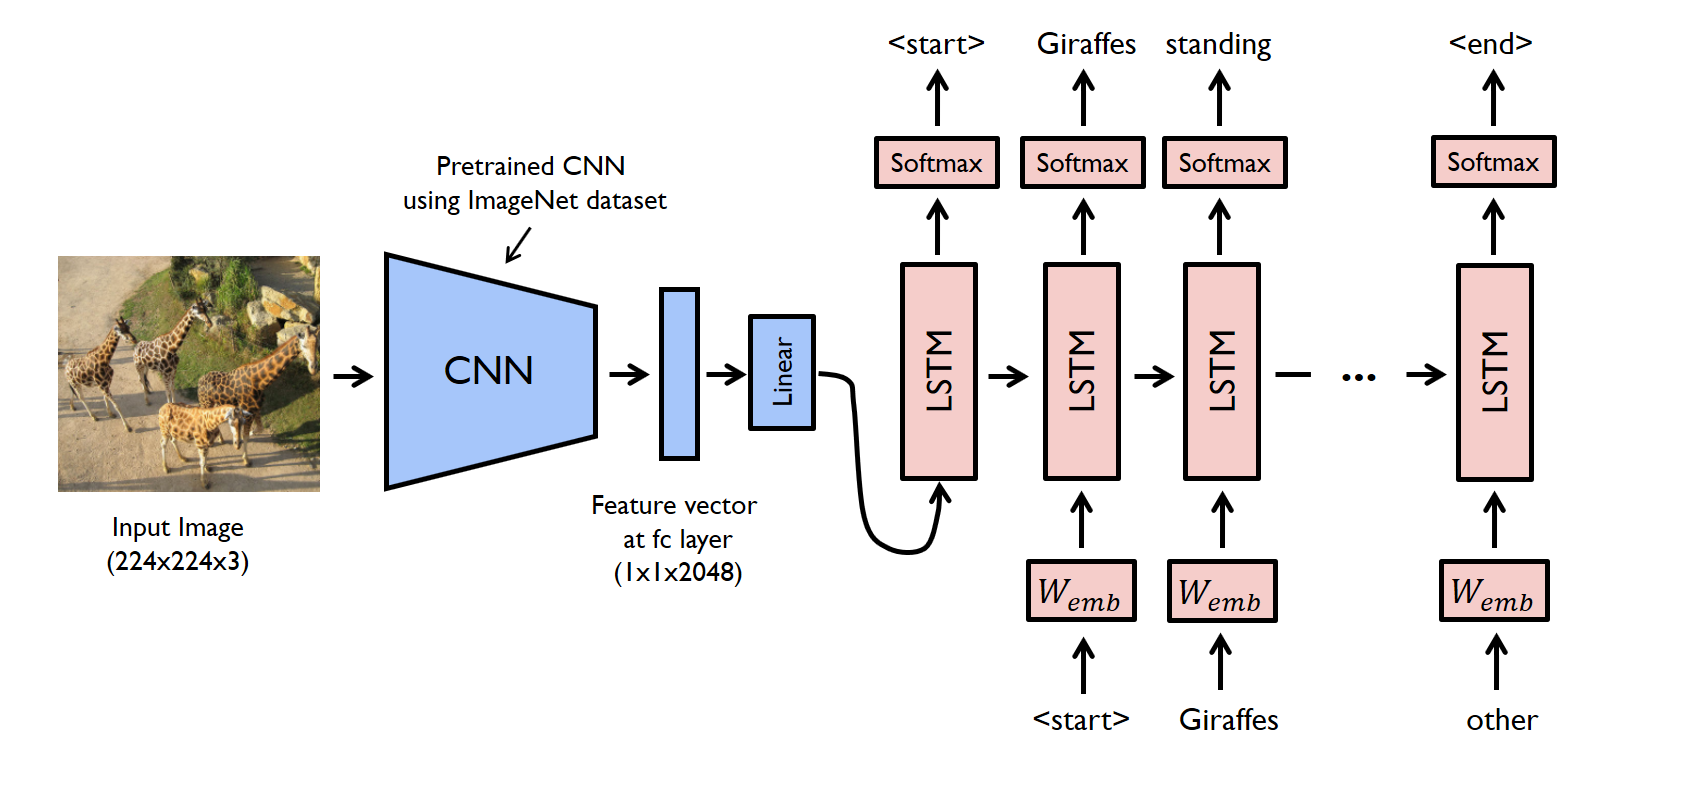
\includegraphics[scale=0.3]{images/ch3/cnn-rnn.png}
    \caption{Encoder-decoder combining CNN and LSTM for image captioning. Source:  \href{https://github.com/yunjey/pytorch-tutorial/tree/master/tutorials/03-advanced/image_captioning}{Yunjey Choi's implementation} of the \textit{Show and Tell} model \citep{Vinyals2015}.}
    \label{fig:cnn-rnn}
\end{figure}

A key of this architecture is the use of a CNN that is pre-trained on a challenging image classification task, which is re-purposed as a feature extractor for the caption generating problem (this is called \textit{transfer learning}). Typically, a CNN trained on the ImageNet dataset is used for this purpose.

For the decoder, most systems proposed so far use LSTM units, since they are more powerful than other types of recurrent units, although lately, GRU units have also emerged as a viable alternative with similar capabilities bu reduced cost.

\subsection{Sequence to Sequence  modelling}\label{subsec:seq2seq}

Next, we delve into the case where both the encoder and decoder are recurrent networks and is commonly known as sequence-to-sequence modeling.

\paragraph{Seq2seq architecture}
Sequence to sequence modeling, \textit{seq2seq} for short, is based on the encoder-decoder architecture to generate a sequence output for a sequence input. This model was born in the field of language modeling \citep{Sutskever2014}. Broadly speaking, it aims to transform an input sequence (source) to a new one (target) and both sequences can be of arbitrary lengths. Examples of transformation tasks include machine translation between multiple languages in either text or audio, question-answer dialog generation, or even parsing sentences into grammar trees.

The seq2seq model normally has an encoder-decoder architecture, composed of:
\begin{itemize}
    \item An encoder processes the input sequence and compresses the information into a context vector (also known as sentence embedding or “thought” vector) of a fixed length. This representation is expected to be a good summary of the meaning of the whole source sequence.
    \item A decoder is initialized with the context vector to emit the transformed output. The early work only used the last state of the encoder network as the decoder initial state.
\end{itemize}    

Both the encoder and decoder are recurrent neural networks, i.e. using LSTM or GRU units


\cref{fig:rnn-rnn} shows an example of a query answering application that uses the seq2seq model. \cref{fig:seq2seq} shows another example of seq2seq modeling applied to translation.

\begin{figure}[hpt]
    \centering
    \includesvg{images/ch3/seq2seq.svg}
    \caption{The sequence to sequence model architecture.}
    \label{fig:seq2seq}
\end{figure}

The layers in the encoder and the decoder are illustrated in \cref{fig:seq2seq_details}.

\begin{figure}[hpt]
    \centering
    \includesvg{images/ch3/seq2seq-details.svg}
    \caption{Layers in seq2seq model.}
    \label{fig:seq2seq_details}
\end{figure}

\paragraph{Seq2seq encoder}
In the encoder, we use the word embedding layer to obtain a feature index from the word index of the input language and then input it into a multi-level recurrent layer, typically made of gated recurrent units such as LSTM or GRU. The input for the encoder is a batch of sequences, which is 2-D tensor with shape (batch size, sequence length). The output consists of both the outputs of the recurrent units and the hidden states (and memory cells of the last time step if using LSTM).

The output shape returned by the encoder after performing forward calculation on the input is (number of time steps, batch size, number of hidden units). The shape of the multi-layer hidden state of the gated recurrent unit in the final time step is (number of hidden layers, batch size, number of hidden units). If GRU is used the \textit{state}  contains only one element, which is the hidden state. If LSTM is used, the \textit{state} list will also contain another element, which is the memory cell.

\paragraph{Seq2seq decoder}
We directly use the hidden state of the encoder in the final time step as the initial hidden state of the decoder. This requires that the encoder and decoder RNNs have the same numbers of layers and hidden units.

The forward calculation of the decoder is similar to the encoder's calculation. The only difference is the addition of a dense layer with the hidden size to be the vocabulary size to output the predicted confidence score for each word.

\paragraph{Seq2seq training}

For each time step, the decoder outputs a vocabulary size confident score vector to predict words. Similar to language modeling, we can apply \textit{softmax} to obtain the probabilities and then use cross-entropy loss to calculate the loss. 

But note that we padded the target sentences to make them have the same length. We would not like to compute the loss on the padding symbols. To solve that, a masked version of the loss function is used.

During training, if the target sequence has length $n$, we feed the first $n-1$ tokens into the decoder as inputs, and the last $n-1$ tokens are used as ground truth label. This is called \textit{Teacher Forcing}, and is depicted in \cref{fig:seq2seq}.

\paragraph{Seq2sea prediction}

To predict a new sequence, the generation process is started by feeding the same "<bos>" token to the decoder at time step 0,  exactly as is done in the training stage. But the input token for a later time step is the predicted token from the previous time step, instead of the ground truth token used during training with the Teacher forcing algorithm. This process is shown in \cref{fig:seq2seq_predict}.

\begin{figure}[hpt]
    \centering
    \includesvg{images/ch3/seq2seq_predict.svg}
    \caption{Sequence to sequence model predicting with greedy search.}
    \label{fig:seq2seq_predict}
\end{figure}

Various approaches exist to predict the next token. For example, in Greedy search, the token with the highest score at each time step is chosen and used to predict the next token. More details on this will be provided in the next chapter when describing our own model details.

\subsection{Attention mechanisms}

A recent trend in Deep Learning is the use of attention mechanisms, typically added to the decoder in an encoder-decoder architecture. 

Attention is, to some extent, motivated by how we pay visual attention to different regions of an image or correlate words in one sentence. Human visual attention is well-studied and while there exist different models, all of them essentially come down to being able to focus on a certain region of an image with "high resolution" while perceiving the surrounding image in "low resolution", and then adjusting the focal point over time. Given a small patch of an image, pixels in the rest provide clues about what should be displayed there. For example, if we see an eye besides a nose, we expect to see another eye at the opposite side of the nose. Similarly, we can explain the relationship between words in one sentence or a close context. When we see "eating", we expect to encounter a food word very soon. 

Attention in Neural Networks has a long history, particularly in image recognition, but only recently have attention mechanisms made their way into recurrent neural networks architectures that are typically used in NLP, and increasingly also in computer vision tasks.

\subsubsection{Attention in Neural Machine Translation}

In the original seq2seq model (\cref{subsec:seq2seq}), the source sequence is encoded into a fixed length context vector that is then passed to the decoder to generate a target sequence. A critical and apparent disadvantage of the fixed-length context vector design of the initial seq2seq model lies in its incapability of remembering long sentences. Often it has forgotten the first part once it completes processing the whole input. The attention mechanism was proposed by \citet{Bahdanau2015} to resolve this weakness. 

Besides, often, a token in the target sequence may closely relate to some tokens in the source sequence instead of the whole source sequence. For example, when translating "Hello world." to "Bonjour le monde.", "Bonjour" maps to "Hello" and "monde" maps to "world".  In the seq2seq model, the decoder may implicitly select the corresponding information from the state passed by the decoder. The attention mechanism, however, makes this selection explicit.

Below we describe the attention mechanism as originally proposed by \citeauthor{Bahdanau2015}, and then we will present a more general model of attention which can be applied to multimodal information tasks such as image captioning, which combines both visual and textual information.

The attention mechanism was born to help memorize long source sentences in neural machine translation (NMT). Rather than building a single context vector out of the encoder’s last hidden state, the secret sauce invented by attention is to create shortcuts between the context vector and the entire source input. The weights of these shortcut connections are customizable for each output element.

While the context vector has access to the entire input sequence, we don’t need to worry about forgetting. The alignment between the source and target is learned and controlled by the context vector. Essentially the context vector consumes three pieces of information: encoder hidden states, decoder hidden states, and alignment between source and target.

\begin{figure}[hpt]
    \centering
    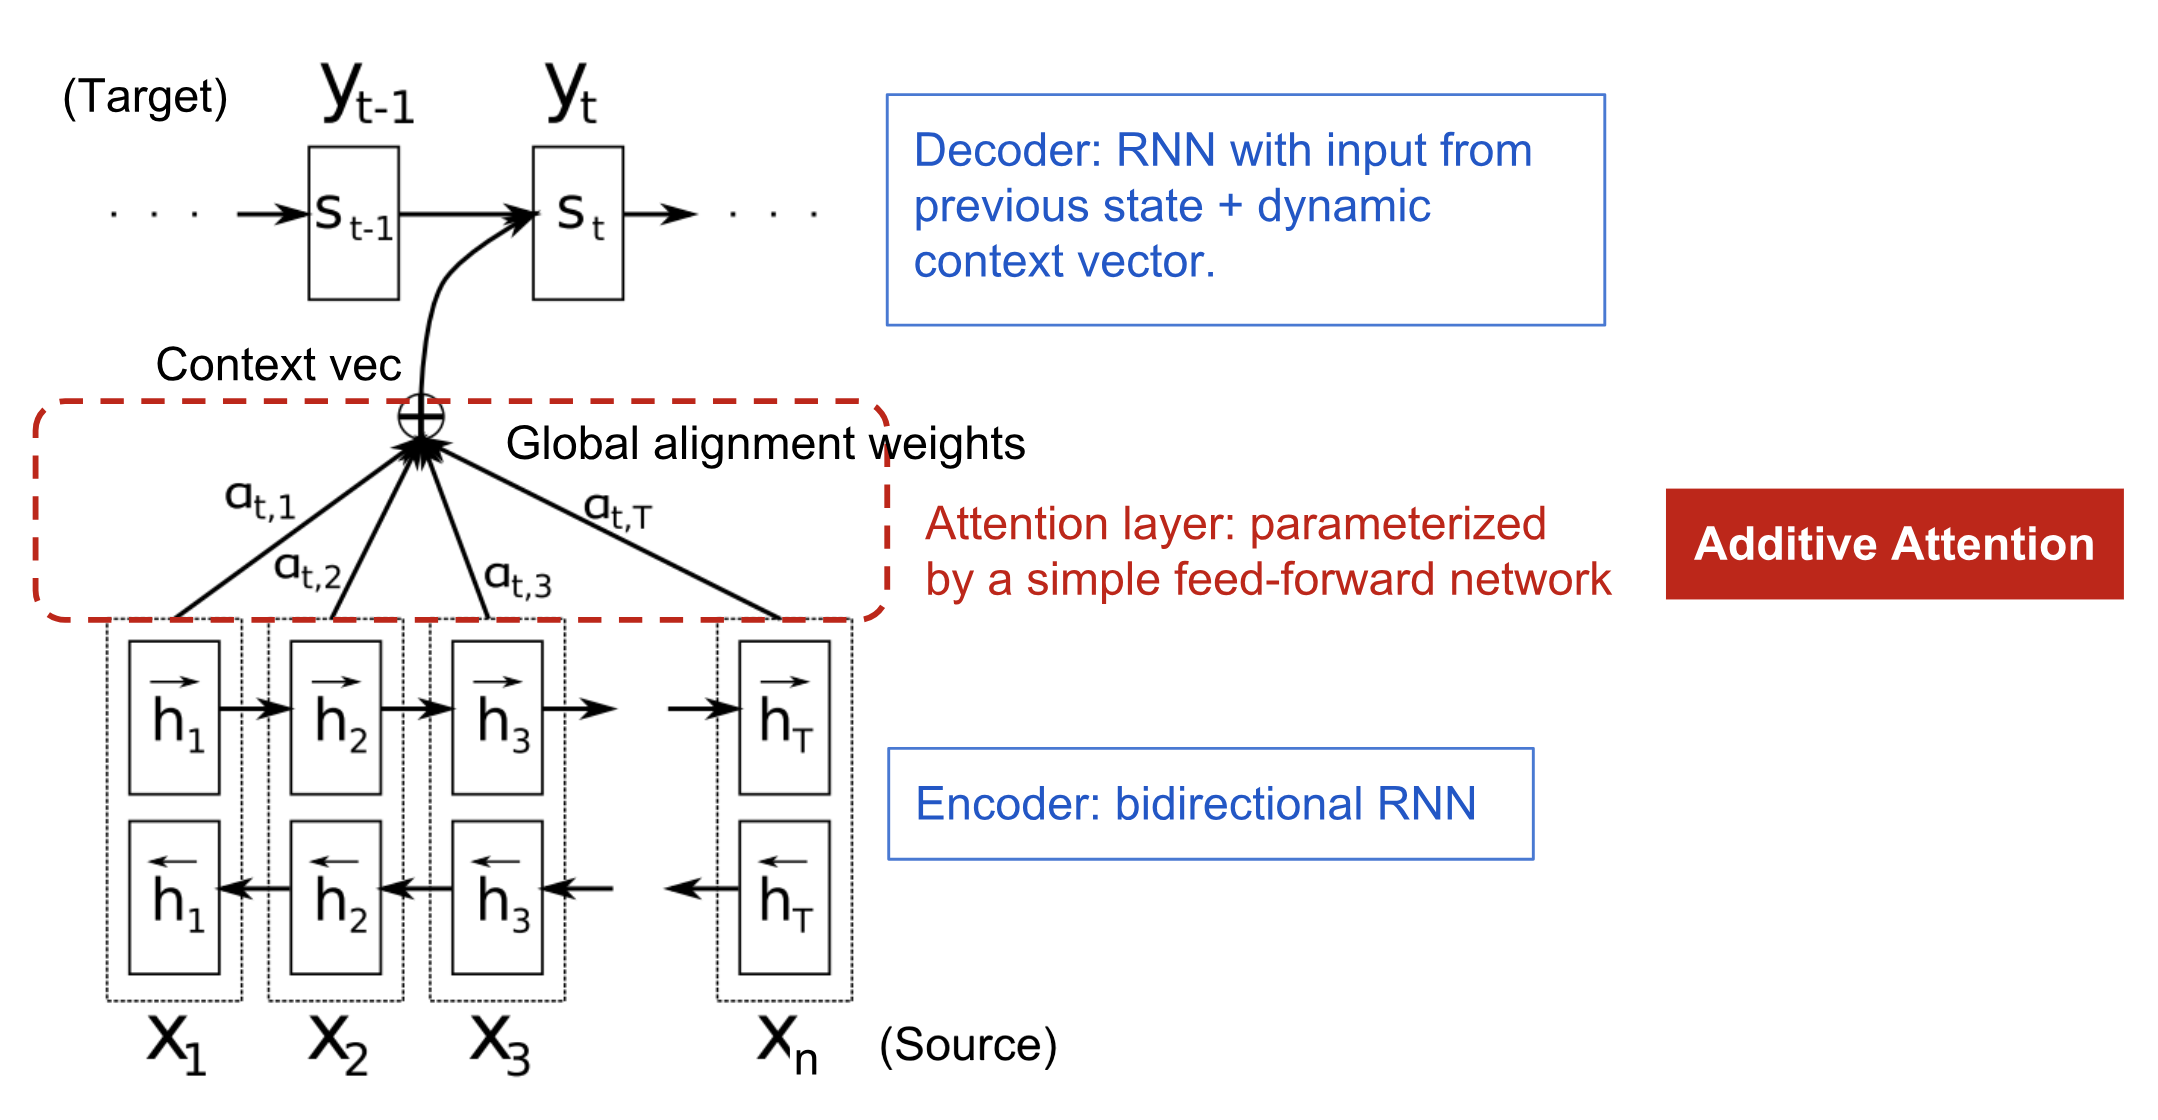
\includegraphics[scale=0.35]{images/ch3/bahdanau-attention.png}
    \caption{The encoder-decoder model with additive attention mechanism in \citep{Bahdanau2015}}
    \label{fig:bahdanau-attention}
\end{figure}

More formally: say, we have a source sequence $\mathbf{x}$ of length $n$ and try to output a target sequence $\mathbf{y}$ of length $m$:
$$
\begin{aligned}
\mathbf{x} &= [x_1, x_2, \dots, x_n] \\
\mathbf{y} &= [y_1, y_2, \dots, y_m]
\end{aligned}
$$
(Variables in bold indicate that they are vectors; same for everything else in this post.)

The encoder is a bidirectional RNN (or any other recurrent network setting of your choice) with a forward hidden state $\overrightarrow{\boldsymbol{h}}_i$ and a backward one $\overleftarrow{\boldsymbol{h}}_i$. A simple concatenation of two represents the encoder state. The motivation is to include both the preceding and following words in the annotation of one word.

$$
\boldsymbol{h}_i = [\overrightarrow{\boldsymbol{h}}_i^\top; \overleftarrow{\boldsymbol{h}}_i^\top]^\top, i=1,\dots,n
$$

The decoder network has hidden state $\boldsymbol{s}_t=f(\boldsymbol{s}_{t-1}, y_{t-1}, \mathbf{c}_t)$ for the output word at position $t, t=1,\dots,m$, where the context vector $\mathbf{c}_t$ is a sum of hidden states of the input sequence, weighted by alignment scores:
$$
\begin{aligned}
\mathbf{c}_t &= \sum_{i=1}^n \alpha_{t,i} \boldsymbol{h}_i & \small{\text{; Context vector for output }y_t}\\
\alpha_{t,i} &= \text{align}(y_t, x_i) & \small{\text{; How well two words }y_t\text{ and }x_i\text{ are aligned.}}\\
&= \frac{\exp(\text{score}(\boldsymbol{s}_{t-1}, \boldsymbol{h}_i))}{\sum_{i'=1}^n \exp(\text{score}(\boldsymbol{s}_{t-1}, \boldsymbol{h}_{i'}))} & \small{\text{; Softmax of some predefined alignment score.}}.
\end{aligned}
$$

The alignment model assigns a score $\alpha_{t,i}$ to the pair of input at position i and output at position $t, (y_t, x_i)$, based on how well they match. The set of $\{\alpha_{t, i}\}$ are weights defining how much of each source hidden state should be considered for each output. In \citep{Bahdanau2015}, the alignment score $\alpha$ is parameterized by a feed-forward network with a single hidden layer and this network is jointly trained with other parts of the model. The score function is therefore in the following form, given that \textit{tanh} is used as the non-linear activation function:

$$\text{score}(\boldsymbol{s}_t, \boldsymbol{h}_i) = \mathbf{v}_a^\top \tanh(\mathbf{W}_a[\boldsymbol{s}_t; \boldsymbol{h}_i])$$

where both $\mathbf{v}_a$ and $\mathbf{W}_a$ are weight matrices to be learned in the alignment model.

The matrix of alignment scores is a nice byproduct to explicitly show the correlation between source and target words.

\begin{figure}[hpt]
    \centering
    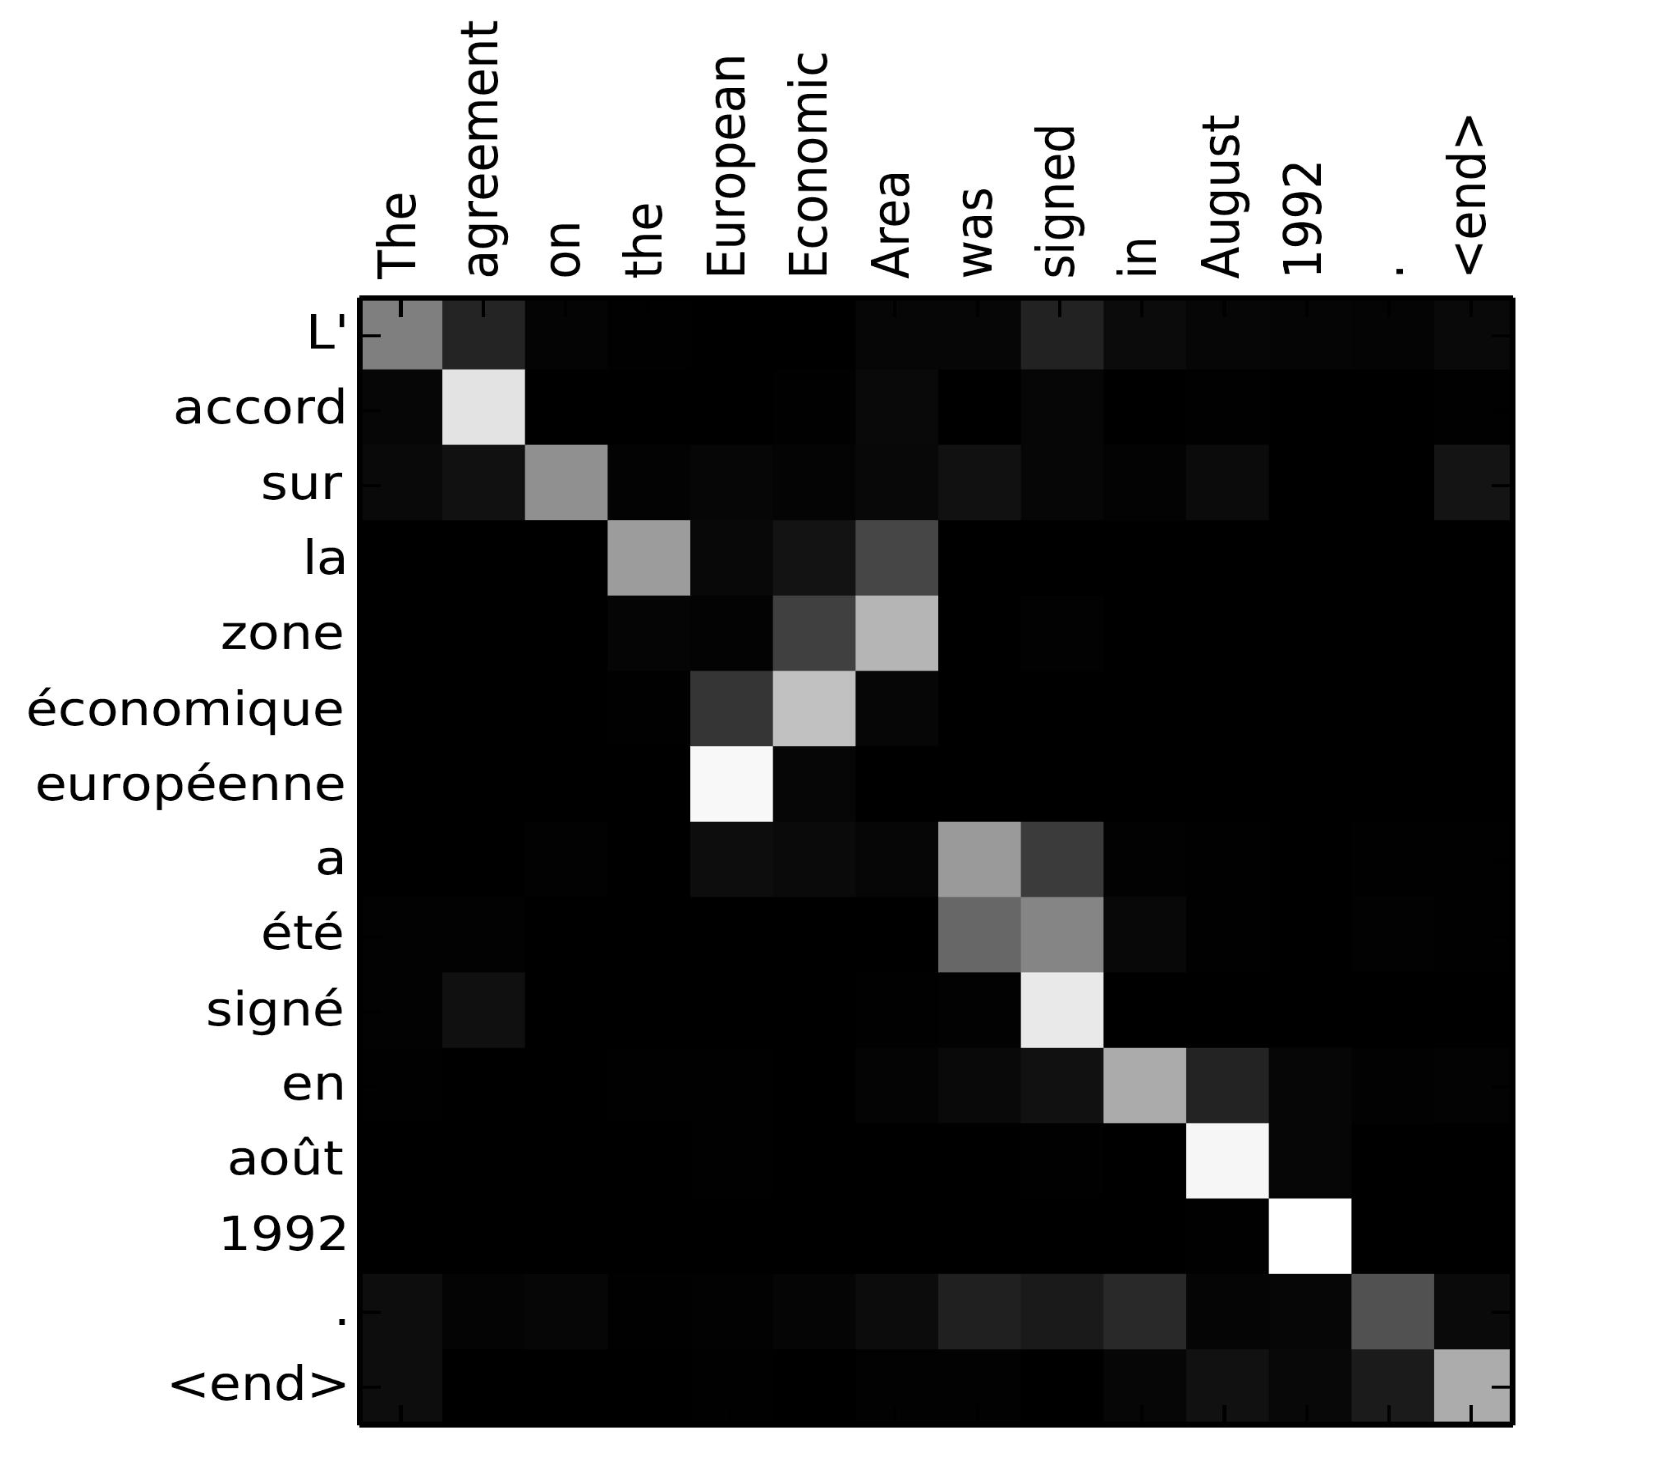
\includegraphics[scale=0.3]{images/ch3/alignment-matrix.png}
    \caption{Alignment matrix of an French sentence and its English translation. Source: Fig 3 in \citep{Bahdanau2015})}
    \label{fig:alignment-matrix}
\end{figure}

\subsubsection{Different attention mechanisms}

With the help of the attention, the dependencies between source and target sequences are not restricted by the in-between distance anymore. Given the big improvement by attention in machine translation, it soon got extended into the computer vision field \citep{Xu2015} and people started exploring various other forms of attention mechanisms \citep{Luong2015, Britz2017, Vaswani2017}.

\cref{tab:attention-mechanisms} enumerates popular attention mechanisms and their corresponding alignment score functions, where $\mathbf{W}_a$ is a trainable weight matrix in the attention layer. 

\begin{table}[hpt]
\caption{summary table of several popular attention mechanisms and corresponding alignment score functions}
\label{tab:attention-mechanisms}
\begin{tabular}{cll}
Name & Alignment score function & Citation \\
\hline
Content-based att. & $\text{score}(\boldsymbol{s}_t, \boldsymbol{h}_i) = \text{cosine}[\boldsymbol{s}_t, \boldsymbol{h}_i]$ & \citep{Graves2014} \\
Additive & $\text{score}(\boldsymbol{s}_t, \boldsymbol{h}_i) = \mathbf{v}_a^\top \tanh(\mathbf{W}_a[\boldsymbol{s}_t; \boldsymbol{h}_i])$ & \citep{Bahdanau2015} \\
Location-Base & $\alpha_{t,i} = \text{softmax}(\mathbf{W}_a \boldsymbol{s}_t)$ & \citep{Luong2015} \\
General & $\text{score}(\boldsymbol{s}_t, \boldsymbol{h}_i) = \boldsymbol{s}_t^\top\mathbf{W}_a\boldsymbol{h}_i$ & \citep{Luong2015} \\
Dot-Product & $\text{score}(\boldsymbol{s}_t, \boldsymbol{h}_i) = \boldsymbol{s}_t^\top\boldsymbol{h}_i$ & \citep{Luong2015} \\
Scaled Dot-Product & $\text{score}(\boldsymbol{s}_t, \boldsymbol{h}_i) = \frac{\boldsymbol{s}_t^\top\boldsymbol{h}_i}{\sqrt{n}}$  & \citep{Vaswani2017}
\end{tabular}
\end{table}

\paragraph{Notes} \textit{Additive} attention is also referred to as \textit{additive} or \textit{concat} by other authors. \textit{Location-based} attention simplifies the softmax alignment to only depend on the target position. The \textit{scaled dot attention} is very similar to the dot-product attention except for the scaling factor $1/\sqrt{n}$; where $n$ is the dimension of the source hidden state.

Besides the scoring functions, there are different ways to classify attention mechanisms, for example:

\begin{itemize}
    \item Self-Attention \citep{Cheng2016}: Relating different positions of the same input sequence. Theoretically, the self-attention mechanism can adopt any score functions above, but just replace the target sequence with the same input sequence. 
    \item Global/Soft \cite{Xu2015}: Attending to the entire input state space. 
    \item Local/Hard \citep{Xu2015, Luong2015}: Attending to the part of input state space; i.e. a patch of the input image.
\end{itemize}

\subsubsection{Self-Attention}

Self-attention, also known as intra-attention, is an attention mechanism relating different positions of a single sequence in order to compute a representation of the same sequence. It has been shown to be very useful in machine reading, abstractive summarization, or image description generation.

The LSTM network by \citet{Cheng2016} uses self-attention to do machine reading. \cref{fig:self-attention} illustrates this mechanism with an example. See how self-attention mechanism enables the model to learn the correlation between the current words and the previous part of the sentence.

\begin{figure}[hpt]
    \centering
    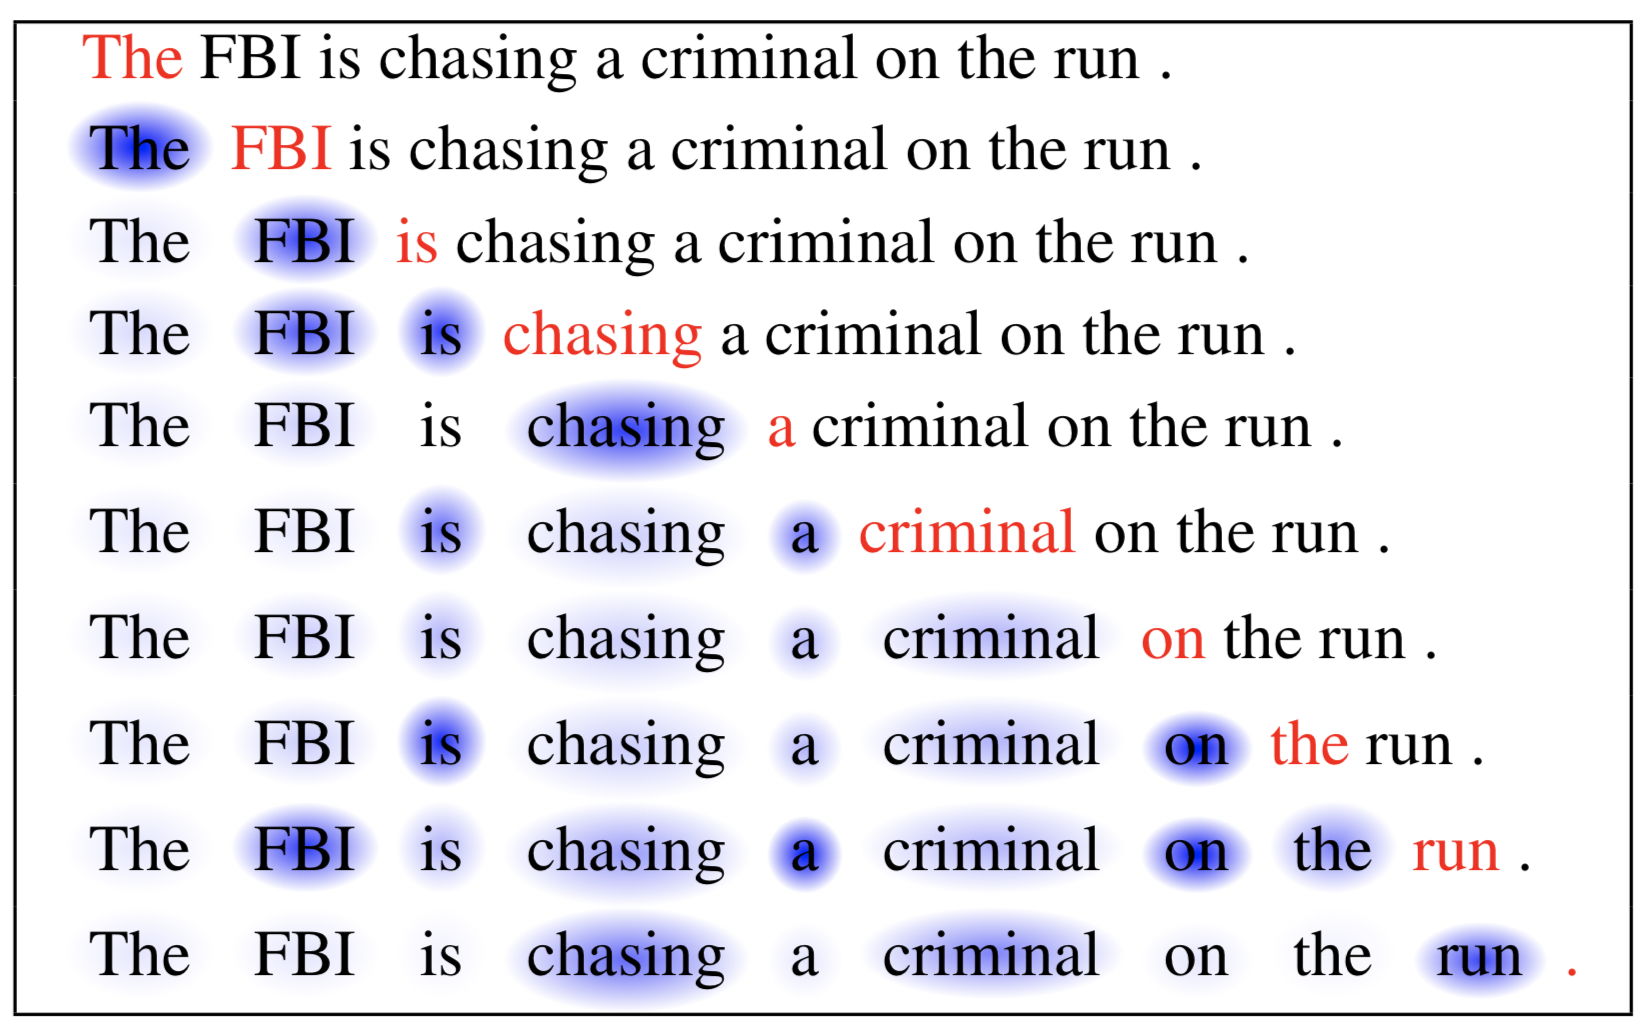
\includegraphics[scale=0.2]{images/ch3/self-attention.png}
    \caption{The current word is in red and the size of the blue shade indicates the activation level. Source: \citep{Cheng2016}.}
    \label{fig:self-attention}
\end{figure}

Self-attention can also be applied to image captioning. For example, in the "Show, attend and tell" paper by \citet{Xu2015}, an input image is first encoded by a convolutional neural network to generate a feature map, and then a recurrent network with self-attention over the image consumes the attention-weighted feature maps to generate the descriptive words one by one. The visualization of the attention weights clearly demonstrates which regions of the image the model pays attention to so as to output a certain word.

\begin{figure}[hpt]
    \centering
    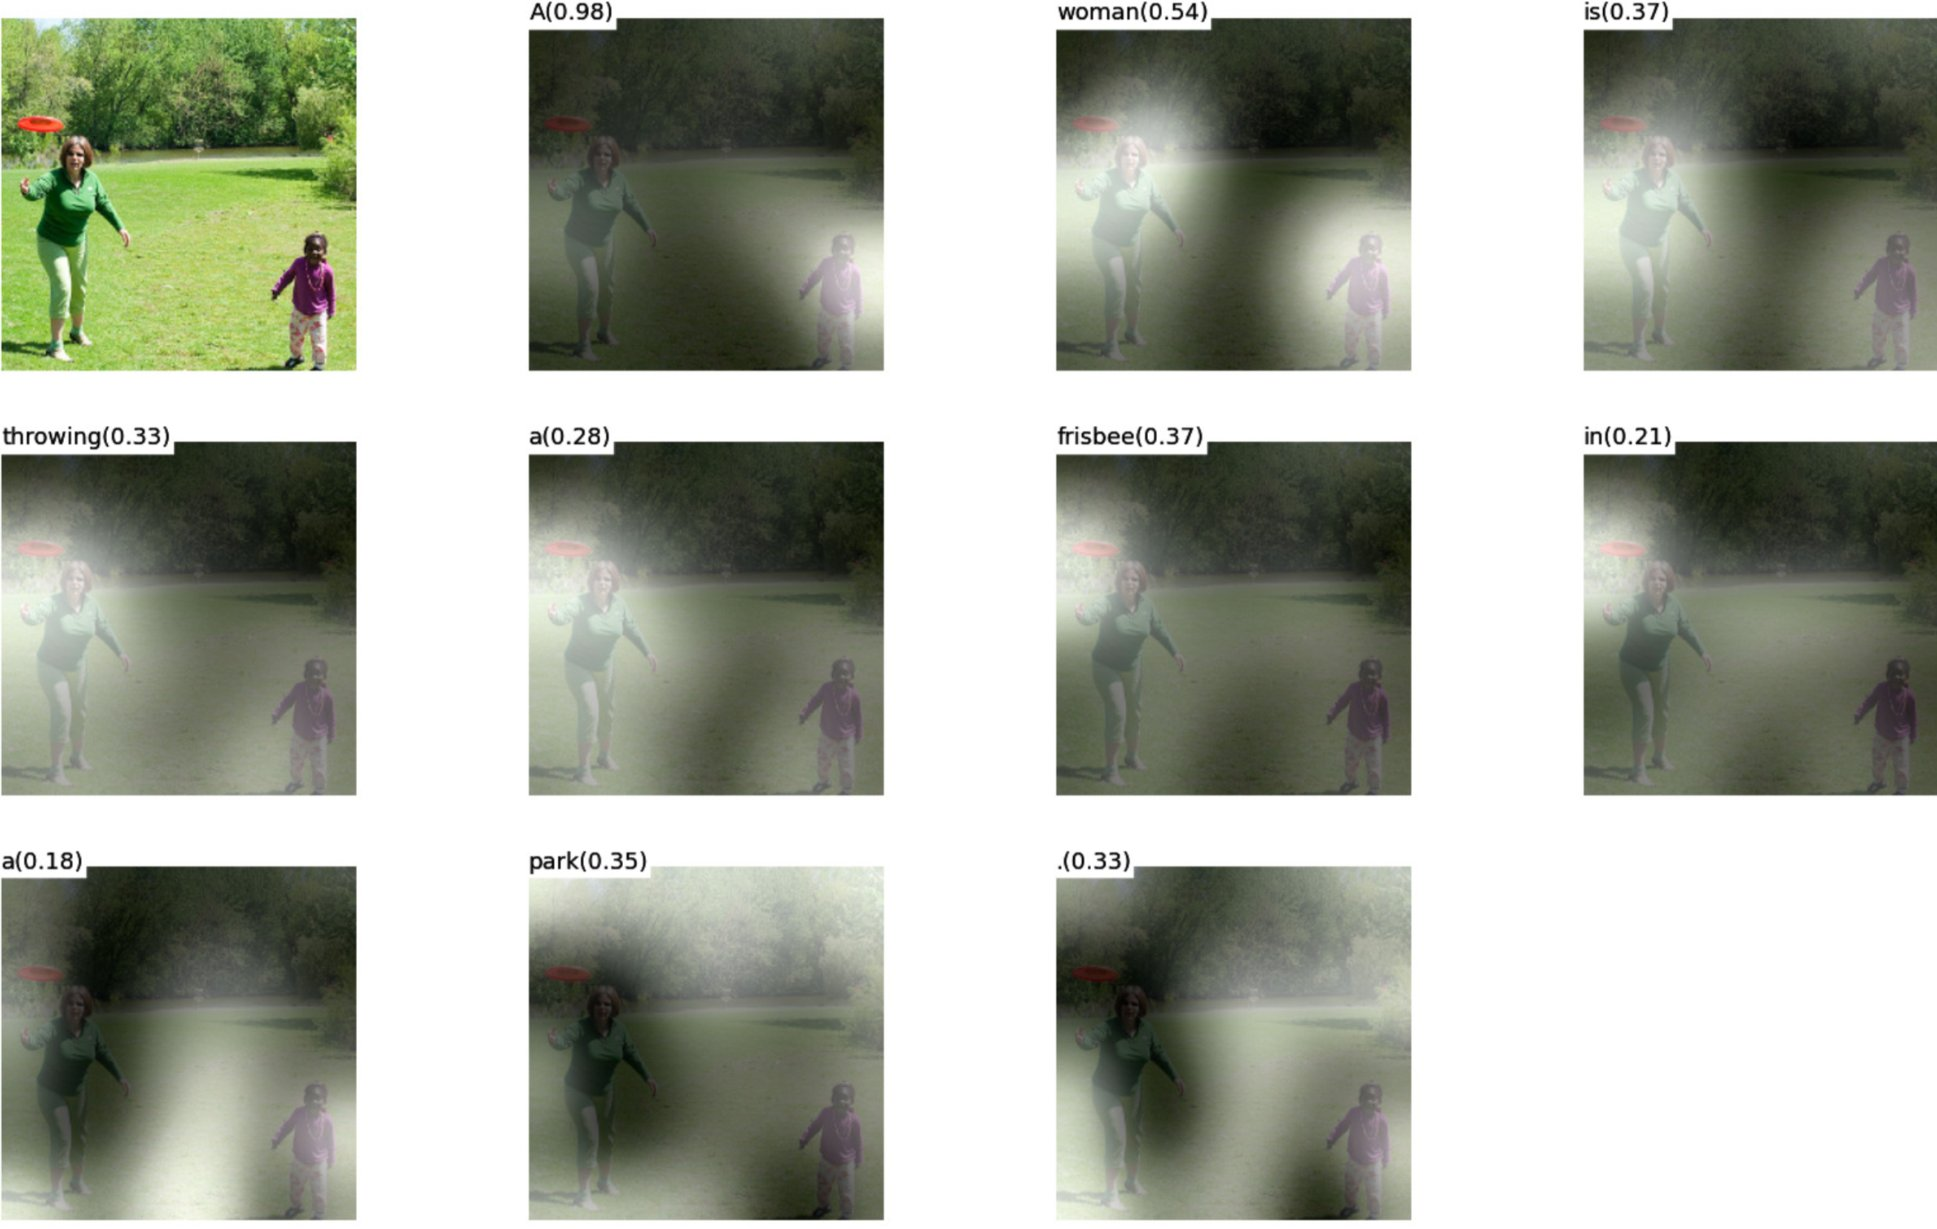
\includegraphics[scale=0.2]{images/ch3/visual-attention.jpg}
    \caption{Caption generation example:A woman is throwing a frisbee in a park. Source: \citep{Xu2015}.}
    \label{fig:visual-attention}
\end{figure}

\subsubsection{Soft vs Hard Attention}

The \textit{soft} vs \textit{hard} attention is another way to categorize how attention is defined. The original idea was proposed in the "Show, attend and tell" paper \citep{Xu2015}, based on whether the attention has access to the entire image or only a patch:

\begin{itemize}
    \item Soft Attention: the alignment weights are learned and placed "softly" over all patches in the source image; which corresponds to the additive attention model by \citet{Bahdanau2015}.
    \begin{itemize}
        \item Pro: the model is smooth and differentiable.
        \item Con: expensive when the source input is large.
    \end{itemize}
    \item Hard Attention: only selects one patch of the image to attend to at a time.
    \begin{itemize}
        \item Pro: less calculation at the inference time.
        \item Con: the model is non-differentiable and requires more complicated techniques such as variance reduction or reinforcement learning to train \citep{Luong2015}. 
    \end{itemize}
\end{itemize}

\cref{fig:soft-vs-hard-attention} illustrates the soft vs hard effect attention with a visual example from the original paper.

\begin{figure}[hpt]
    \centering
    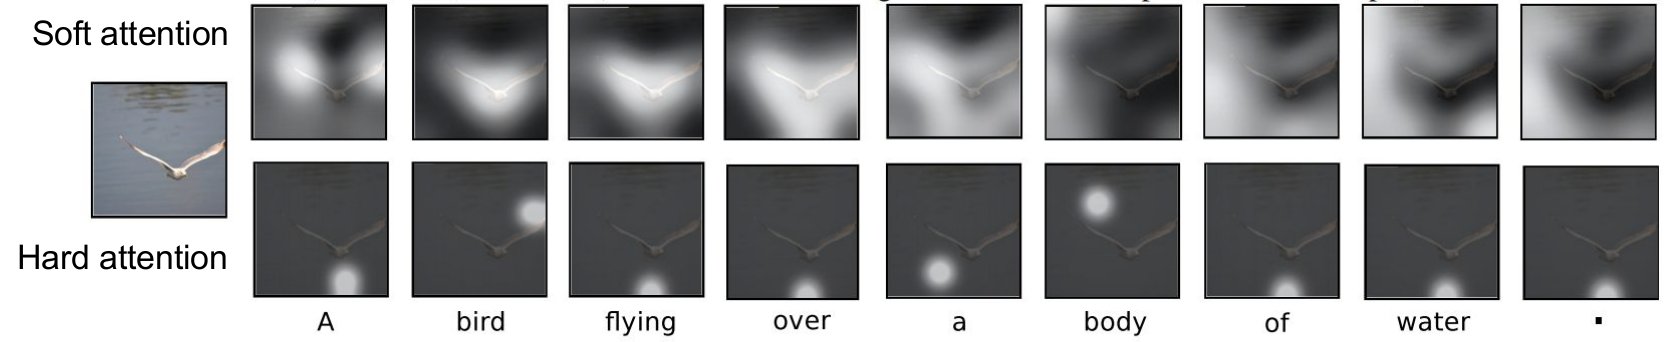
\includegraphics[scale=0.3]{images/ch3/soft-vs-hard-attention.png}
    \caption{Comparative of soft (top) vs hard (bottom) attention during caption generation. Source: \citep{Xu2015}.}
    \label{fig:soft-vs-hard-attention}
\end{figure}

\subsubsection{Global vs Local Attention}

\citet{Luong2015} coined the \textit{global} vs \textit{local} attention distinction. The global attention is similar to the soft attention, while the local one is an interesting blend between hard and soft, an improvement over the hard attention to make it differentiable: the model first predicts a single aligned position for the current target word and a window centered around the source position is then used to compute a context vector.

\cref{fig:global-vs-local-attention} compares global and local models of attention in a seq2seq setup.

\begin{figure}[hpt]
    \centering
    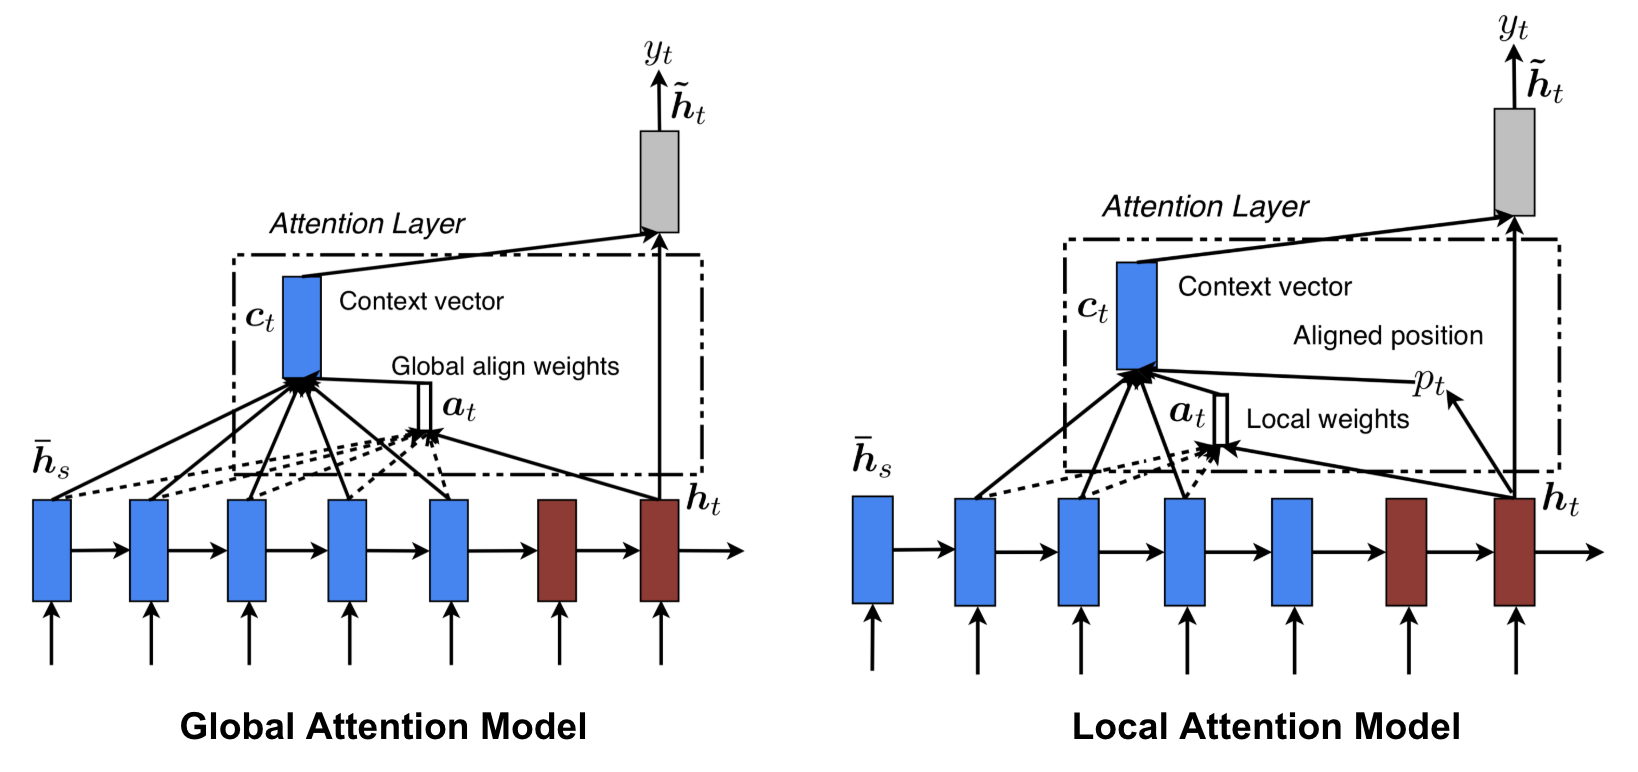
\includegraphics[scale=0.3]{images/ch3/global-vs-local-attention.png}
    \caption{Comparative of global (left) vs local (right) attention in the seq2seq model. Source: \citep{Luong2015}.}
    \label{fig:global-vs-local-attention}
\end{figure}

The are other models that apply similar ideas and can thus be seen as variations of the same idea. We will not describe them here, but we enumerate them together:

\begin{itemize}
    \item The \textit{Neural Turing Machine}(NTM), by \citet{Graves2014}, is a model architecture for coupling a neural network with external memory storage. The memory mimics the Turing machine tape and the neural network controls the operation heads to read from or write to the tape. However, the memory in NTM is finite, and thus it probably looks more like a "Neural von Neumann Machine".
    \item In problems like sorting or traveling salesman, both input and output are sequential data. Unfortunately, they cannot be easily solved by classic seq2seq or NMT models, given that the discrete categories of output elements are not determined in advance, but depends on the variable input size. The \textit{Pointer Net} (Ptr-Net), was proposed by \citet{Vinyals2015} to address this problem when the output elements correspond to positions in an input sequence. Rather than using attention to blend hidden units of an encoder into a context vector (See Fig. 8), the Pointer Net applies attention over the input elements to pick one as the output at each decoder step.
    \item The \textit{transformer} model introduced in the "Attention is all you need" paper by \citet{Vaswani2017} is entirely built on the self-attention mechanisms without using sequence-aligned recurrent architecture. It presented a lot of improvements to the soft attention mechanism, and make it possible to do seq2seq modeling without recurrent network unit, thus reducing the computational costs.
\end{itemize}

% \subsection{A general model of attention}\label{subsec:general-attention-model}

% Formally, attention is a \textit{generalized pooling method with bias alignment over inputs}. The core component in the attention mechanism is the \textbf{attention layer}. An input of the attention layer is called a \textbf{query}. For a query, the attention layer returns the output based on its \textbf{memory}, which is a set of key-value pairs. To be more specific, assume a query $\mathbf{q}\in\mathbb R^{d_q}$, and the memory contains $n$ key-value pairs, $(\mathbf{k}_1, \mathbf{v}_1), \ldots, (\mathbf{k}_n, \mathbf{v}_n)$, with $\mathbf{k}_i\in\mathbb R^{d_k}$, $\mathbf{v}_i\in\mathbb R^{d_v}$. The attention layer then returns an output $\mathbf o\in\mathbb R^{d_v}$ with the same shape, such that each key has a value.

% \begin{figure}[hpt]
%     \centering
%     \includesvg{images/ch3/attention.svg}
%     \caption{The attention layer returns an output based on the input query and its memory.}
%     \label{fig:attention}
% \end{figure}

% To compute the output, we first assume there is a score function $\alpha$ which measures the similarity --\textit{alignment}-- between the query and a key. Then we compute all $n$ scores $a_1, \ldots, a_n$ by

% $$a_i = \alpha(\mathbf q, \mathbf k_i).$$

% Next we use \textit{softmax} to obtain the attention weights

% $$b_1, \ldots, b_n = \textrm{softmax}(a_1, \ldots, a_n).$$

% The output is then a weighted sum of the values

% $$\mathbf o = \sum_{i=1}^n b_i \mathbf v_i.$$

% Different choices of the score function lead to different attention layers, as the ones shown in \cref{tab:attention-mechanisms}. 

% Below we see how this general model fits some of the specific models introduced above, More specifically, we briefly describe two of the most popular attention models: the \textit{dot product} and the \textit{additive} models. 

% \subsubsection{Scaled Dot Product Attention}

% The dot product assumes the query has the same dimension than the keys, namely $\mathbf q, \mathbf k_i \in\mathbb R^d$ for all $i$. It computes the score by an inner product between the query and a key, and often then divided by $\sqrt{d}$ to make the scores less sensitive to the dimension $d$. In other words,

% $$\alpha(\mathbf q, \mathbf k) = \langle \mathbf q, \mathbf k \rangle /\sqrt{d}.$$

% Assume $\mathbf Q\in\mathbb R^{m\times d}$ contains $m$ queries and $\mathbf K\in\mathbb R^{n\times d}$ has all $n$ keys. We can compute all $mn$ scores by

% $$\alpha(\mathbf Q, \mathbf K) = \mathbf Q \mathbf K^T /\sqrt{d}.$$

% This attention mechanism could also include a dropout regularization mechanism (to randomly drop some attention weights).

% \subsubsection{Additive attention (Multilayer Perception)}

% Multilayer perception attention was proposed by \citet{Bahdanau2015} for seq2seq modeling. In this form of attention, we first project both query and keys into a common feature space $h$.

% To be more specific, assume learnable parameters $\mathbf W_k\in\mathbb R^{h\times d_k}$, $\mathbf W_q\in\mathbb R^{h\times d_q}$, and $\mathbf v\in\mathbb R^{p}$, then the score function is defined by

% $$\alpha(\mathbf k, \mathbf q) = \mathbf v^T \text{tanh}(\mathbf W_k \mathbf k + \mathbf W_q\mathbf q). $$

% It equals to concatenate the key and value in the feature dimension, and then feed them into a hidden-layer perception with hidden size $h$ and output size $1$. The hidden layer activation function is \textit{tanh}, and no bias is applied.

% \subsubsection{Sequence to Sequence with Additive Attention}

% In this section, we add the attention mechanism to the sequence to sequence model introduced in \cref{subsec:seq2seq} to explicitly select the state. The following figure shows the model architecture for a decoding time step. As can be seen, the memory of the attention layer consists of the encoder outputs of each time step. During decoding, the decoder output from the previous time step is used as the query, the attention output is then fed into the decoder with the input to provide attentional context information.

% \begin{figure}[hpt]
%     \centering
%     \includesvg{images/ch3/seq2seq_attention.svg}
%     \caption{The second time step in decoding for the sequence to sequence model with attention mechanism.}
%     \label{fig:seq2seq_attention}
% \end{figure}

% The layer structure in the encoder and the decoder is shown in the following figure.

% \begin{figure}[hpt]
%     \centering
%     \includesvg{images/ch3/seq2seq-attention-details.svg}
%     \caption{Layers in seq2seq model with attention.}
%     \label{fig:seq2seq-attention-details}
% \end{figure}

% For the decoder of this model, we add an MLP attention layer which has the same hidden size as the LSTM layer. The state passed from the encoder to the decoder contains three items:

% \begin{itemize}
%     \item the encoder outputs of all time steps, which are used as the attention layer's memory with identical keys and values
%     \item the hidden state of the last time step that is used to initialize the encoder's hidden state  
%     \item valid lengths of the decoder inputs so the attention layer will not consider encoder outputs for padding tokens.
% \end{itemize}

% In each time step of decoding, we use the output of the last RNN layer as the query for the attention layer. Its output is then concatenated with the input embedding vector to feed into the RNN layer. Despite the RNN layer's hidden state also contains history information from the decoder, the attention output explicitly selects the encoder outputs that are correlated to the query and suspends other non-correlated information.

% The training loss is similar to the seq2seq model because the sequences in the training dataset are relatively short. The additional attention layer doesn’t lead to a significant difference. But due to both attention layer computational overhead and we unroll the time steps in the decoder, this model is much slower than the seq2seq model without attention.



\chapter{Datasets}
\label{chapter:datasets}
\chapter{Models}
\label{chapter:models}
%\input{6_evaluation.tex}
%\input{7_conclusions.tex}

% bibliografia
\addcontentsline{toc}{chapter}{Bibliography}
\bibliographystyle{plain}
\bibliography{references}

\end{document}